% ============================================================
%  Topical Burstiness in Literary Texts:
%  A Semantic Trajectory Approach
%
%  M. Degli Esposti, M. A. Montemurro
%  Target: Physica A
% ============================================================

\documentclass[12pt,a4paper]{article}

% ---- Packages ----------------------------------------------
\usepackage{amsmath,amssymb,amsthm}
\usepackage{graphicx}
\graphicspath{{../}{./}}
\usepackage{xcolor}
\usepackage{booktabs}
\usepackage{algorithm}
\usepackage{algpseudocode}
\usepackage{natbib}
\usepackage{microtype}
\usepackage{placeins}
\usepackage{rotating}
\usepackage{geometry}
\usepackage{hyperref}
\geometry{margin=2.5cm}



% ---- Theorem environments -----------------------------------
\newtheorem{proposition}{Proposition}
\newtheorem{corollary}{Corollary}
\newtheorem{remark}{Remark}

% ---- Custom commands ----------------------------------------
\newcommand{\bk}{B_k}
\newcommand{\lk}{\lambda_k}
\newcommand{\xtk}{x_t^{(k)}}
\newcommand{\vk}{\mathbf{v}_k}
\newcommand{\et}{\mathbf{e}_t}
\newcommand{\ebar}{\bar{\mathbf{e}}}
\newcommand{\Sig}{\boldsymbol{\Sigma}}
\newcommand{\R}{\mathbb{R}}
\newcommand{\meantau}{\langle\tau\rangle}
\newcommand{\sigmatau}{\sigma_\tau}
\newcommand{\CV}{\mathrm{CV}}
\newcommand{\TODO}[1]{\textcolor{red}{\textbf{[TODO: #1]}}}
\newcommand{\NOTE}[1]{\textcolor{blue}{\textbf{[NOTE: #1]}}}

\usepackage{totcount}
\newtotcounter{todocount}

% ------------------------------------------------------------
\begin{document}

\title{Semantic burstiness across principal directions\\
       of textual variation}

\author{Mirko Degli Esposti$^{1}$ \and Marcelo A.\ Montemurro$^{2}$\\[6pt]
  \small $^1$Department of Physics and Astronomy,
         University of Bologna, Bologna, Italy\\
  \small $^2$School of Mathematics and Statistics,
         The Open University, Milton Keynes, UK}

\date{\small Draft --- \today}

\maketitle

% -----------------------------------------------------------------------------
\begin{abstract}
Long-range correlations in written texts extend over scales far beyond
local syntax, but their relation to semantic organisation remains
incompletely understood. Previous work has linked these correlations to
the bursty recurrence of topically relevant words. Here we generalise
that construction from individual lexical items to distributed semantic
observables. We map a text token by token onto a trajectory of
pre-trained word embeddings, use principal component analysis to
identify text-specific directions of semantic variation, and threshold
the projected series to define inter-event times; their coefficients of
variation form a component-resolved burstiness spectrum $\{B_k\}$.
Across 16 literary and scientific texts and the first 20 components,
the originals remain systematically above the geometric
inter-event-time baseline and above two complementary controls: a
word-shuffled null, which preserves the embedding covariance, the PCA
eigensystem and the marginal projected distributions while destroying
temporal order, and a fractional-Gaussian-noise surrogate, which
preserves the Zipfian frequency structure and matches the DFA exponent
of the original rank sequence. At $q=0.95$ the original exceeds both
controls in every text--component pair, while the two controls are
statistically indistinguishable from each other. Autocorrelation and
detrended fluctuation analysis of the semantic projections separate the
originals from both controls in the same way. Global rank-level
long-range correlations are therefore insufficient to generate the
bursty recurrence observed along semantic directions, which instead
requires ordered topical organisation.
\end{abstract}

\smallskip
\noindent\textbf{Keywords:} long-range correlations; burstiness; word
embeddings; PCA; surrogate data; semantic trajectories; complex systems;
topical structure

% -----------------------------------------------------------------------------
\section{Introduction}
\label{sec:intro}

\subsection{Long-range correlations in texts}

Written texts exhibit statistical structure over scales far beyond
local syntactic dependencies.
Among the most robust observations is the presence of long-range
correlations in symbolic sequences derived from natural language.
When a text is encoded as a numerical time series and analysed with
detrended fluctuation analysis (DFA) \citep{Peng1994}, the fluctuation
function commonly scales as $F(L)\sim L^\alpha$, with
$\alpha\in[0.6,0.8]$, above the uncorrelated value $\alpha=0.5$,
across languages, genres, and encoding choices
\citep{Ebeling1995,MontemurroPury2002}.

This observation raises a fundamental question: what aspect of textual
organisation produces memory over hundreds or thousands of tokens?
At least two statistical structures must be distinguished.
The first is static lexical composition, represented by the vocabulary
and word-frequency distribution.
Its most familiar regularity is Zipf's law \citep{Zipf1949}, according
to which the frequency $f(r)$ of the word of rank $r$ follows
$f(r)\sim r^{-\gamma}$ with $\gamma\simeq1$.
The second is the temporal ordering of words, through which syntax,
discourse, argument, and thematic development unfold.
A word-shuffled text preserves lexical composition and Zipf's law but
destroys temporal organisation, causing the DFA exponent to approach
$\alpha=0.5$ \citep{Ebeling1995,MontemurroPury2002}.

The global DFA exponent, however, does not by itself identify the
semantic mechanism responsible for long-range correlations.
The surrogate introduced in \citet{DegliEsposti2025} maps fractional
Gaussian noise (FGN) onto the empirical rank-frequency structure and is
tuned to reproduce the DFA exponent of the original rank sequence.
It therefore provides a stationary, rank-level route to the same global
scaling and allows us to ask whether matching long-range memory in
frequency-rank space is sufficient to reproduce temporal organisation in
semantic space.

A geometric approach to long-range textual structure was introduced by
\citet{AlvarezLacalle2006}.
They constructed a co-occurrence representation within a sliding
``window of attention'' and used singular value decomposition to identify
text-specific concept vectors.
The motion of the sliding window through concept space produced
trajectories with power-law autocorrelation over long textual scales, and
surrogate tests connected this behaviour to hierarchical textual
organisation.
Their work established that semantic dynamics can be studied as motion
through a reduced concept space.

Our approach shares this geometric viewpoint but differs in three
respects.
First, we use pre-trained static word embeddings rather than a
co-occurrence matrix estimated from a single text.
Second, the trajectory is resolved token by token rather than through an
aggregated sliding window.
Third, our primary observable is the burstiness of threshold crossings
along semantic directions, measured through the inter-event-time
coefficient of variation, together with the autocorrelation and DFA of
the projected series.

\subsection{The Altmann et al.\ mechanism}

A mechanism connecting topical organisation to long-range correlations
was developed by \citet{Altmann2012}.
Their framework treats language as a hierarchy of observables, from
topics to words and then to lower-level symbolic representations.
Correlations can propagate down this hierarchy, whereas burstiness is
visible most clearly at semantically relevant levels and can be lost
under projection to lower levels.

Formally, a local matching condition $\alpha$ maps a text to a binary
sequence $u_t^{(\alpha)}\in\{0,1\}$.
For example, $u_t^{(\alpha)}=1$ may indicate that token $t$ is the word
``prince''.
The gaps $\tau$ between successive events define an inter-event-time
(IET) distribution, whose coefficient of variation
\begin{equation}
  \CV=\frac{\sigmatau}{\meantau}
\end{equation}
measures temporal clustering.
Topically relevant words tend to occur in concentrated textual domains
and therefore show broad IET distributions and elevated burstiness,
whereas common function words are distributed more regularly even when
long-range correlations remain visible in lower-level observables.

This framework suggests a natural extension.
A topic such as war, philosophical reflection, biological variation, or
social interaction is not expressed by one keyword alone.
It activates a distributed set of semantically related words.
A suitable topic-level observable should therefore respond to a region
or direction of semantic space rather than to the exact recurrence of a
single word type.

\subsection{Motivation and contribution}

We represent a text as an embedding trajectory
$(\mathbf{e}_t)_{t=1}^M$ in $\R^d$, where each retained token is mapped
to a pre-trained static word vector
\citep{Mikolov2013,Pennington2014}.
PCA of this trajectory identifies an ordered set of orthogonal,
text-specific directions of semantic variation.
Projecting the trajectory onto a direction $\mathbf{v}_k$ yields a
continuous semantic time series; thresholding that series produces a
binary event sequence to which the IET construction of
\citet{Altmann2012} can be applied.
The resulting spectrum $\{B_k\}_{k=1}^K$ measures burstiness separately
along the first $K$ principal semantic directions.

This construction supports a positive, component-resolved question:
how is semantic burstiness distributed across the principal directions
of a text?
The principal components are ordered by variance, but PCA does not
maximise burstiness.
The empirical relation between the eigenvalue spectrum
$\{\lambda_k\}$ and the burstiness spectrum $\{B_k\}$ therefore reveals
whether directions of strong semantic variation are also directions of
strong temporal clustering.
The analyses below show interpretable semantic contrasts along the
leading components, broad IET distributions in the original texts, and
elevated burstiness throughout the first 20 components examined.
They also show that the strength of association between semantic
variance and burstiness is text dependent: the two quantities are
related in some texts but are not interchangeable.

We then use two complementary null models to determine which statistical
properties produce this behaviour.
The word-shuffled null preserves the multiset of embedded tokens and
therefore preserves the empirical covariance, PCA eigensystem, and
marginal projected distributions exactly, while destroying temporal
order.
The FGN surrogate retains the empirical rank-frequency structure and is
tuned to match the original rank-sequence DFA exponent, but generates
that scaling through a stationary rank-level process.
The comparison separates static semantic geometry from ordered semantic
dynamics, and global rank-level memory from burstiness in embedding
space.

Across the analysed corpus, both controls remain close to the geometric
IET baseline, whereas the original text is more bursty across essentially
all text--component pairs and over a broad range of threshold quantiles.
The projected autocorrelation functions and DFA exponents reinforce this
separation: semantic persistence remains visible in the original
trajectory but disappears from both controls, including the FGN
surrogate whose rank sequence retains the original global DFA exponent.
Thus matching lexical frequencies and rank-level long-range scaling is
not sufficient to reproduce semantic burstiness.

\subsection{Structure of the paper}

Section~\ref{sec:theory} develops the theoretical framework, including
semantic projections, PCA, the component-resolved burstiness spectrum,
and the two null models. Section~\ref{sec:pipeline} describes the
computational pipeline. Section~\ref{sec:oliver} presents the Results
for four representative texts, organised around semantic
interpretability, component-resolved burstiness, and threshold
robustness. Section~\ref{sec:corpus} establishes the corpus-level
generality of the component spectra and null-model separation.
Section~\ref{sec:entropy} examines persistence in semantic projection
space using autocorrelation and DFA and gives an information-theoretic
interpretation. Section~\ref{sec:discussion} discusses implications
and limitations.

\section{Theoretical Framework}
\label{sec:theory}

\subsection{From binary indicators to continuous semantic projections}
\label{sec:observables}

Following \citet{Altmann2012}, let a text be a symbolic sequence
$\mathbf{s}=(s_1,s_2,\ldots,s_N)$ over a finite vocabulary
$\mathcal{A}$.
A local matching condition $\alpha$ defines a binary observable
\begin{equation}
  u_t^{(\alpha)}=\mathbf{1}[s_t\text{ satisfies }\alpha].
  \label{eq:binary_indicator}
\end{equation}
The autocorrelation of this sequence and the diffusion exponent
$\gamma$, defined by $\sigma_X^2(t)\sim t^\gamma$ for
$X(t)=\sum_{j=1}^t u_j^{(\alpha)}$, characterise its long-range
structure.

We generalise the local lexical condition to a distributed semantic
observable.
Let $\phi:\mathcal{A}\to\R^d$ be a pre-trained static word embedding.
After preprocessing and embedding lookup, the retained tokens are
relabeled consecutively as $(\tilde s_1,\ldots,\tilde s_M)$, with
$M\leq N$.
Their \emph{embedding trajectory} is
\begin{equation}
  \mathcal{E}=(\et)_{t=1}^M,
  \qquad
  \et=\phi(\tilde s_t).
  \label{eq:trajectory}
\end{equation}

For a unit vector $\mathbf{v}\in\R^d$, the corresponding
\emph{semantic projection} is
\begin{equation}
  x_t^{\mathbf{v}}=(\et-\ebar)\cdot\mathbf{v},
  \qquad
  \ebar=\frac{1}{M}\sum_{t=1}^M\et.
  \label{eq:projection}
\end{equation}
At threshold $\theta$, this continuous series defines the binary event
sequence
\begin{equation}
  b_t^{\mathbf{v}}(\theta)
  =\mathbf{1}\!\left[x_t^{\mathbf{v}}>\theta\right].
  \label{eq:binary_from_proj}
\end{equation}
The projection describes motion along a semantic direction, while the
binary series records visits to its upper tail and supplies the events
whose recurrence statistics are analysed.

\begin{remark}
  If $\mathbf{v}$ is parallel to $\phi(w)-\ebar$ for a word type $w$,
  then $x_t^{\mathbf{v}}$ tends to be large when the current token is
  $w$ and for tokens whose embeddings are close to, or strongly aligned
  with, $\phi(w)$.
  Thresholding this projection therefore gives a softened semantic
  analogue of the exact word indicator in
  Eq.~\eqref{eq:binary_indicator}.
  The construction extends the unit of analysis from one lexical item to
  a distributed semantic neighbourhood.
\end{remark}

\subsection{PCA of the embedding trajectory}
\label{sec:pca}

The direction $\mathbf{v}$ determines the semantic observable.
We use the principal components of the embedding trajectory to obtain a
text-specific orthonormal basis ordered by captured variance.
The empirical covariance matrix of the mean-centred trajectory is
\begin{equation}
  \Sig=
  \frac{1}{M}\sum_{t=1}^M
  (\et-\ebar)(\et-\ebar)^\top
  \in\R^{d\times d}.
  \label{eq:covariance}
\end{equation}
Its eigendecomposition
\begin{equation}
  \Sig\vk=\lk\vk,
  \qquad
  \lambda_1\geq\lambda_2\geq\cdots\geq\lambda_d\geq0,
  \label{eq:pca_eigenproblem}
\end{equation}
yields the principal directions $\vk$ and their variances $\lk$.
The projected series for component $k$ is
\begin{equation}
  \xtk=(\et-\ebar)\cdot\vk,
  \qquad t=1,\ldots,M.
  \label{eq:proj_series}
\end{equation}

PCA directions maximise variance, not semantic interpretability or
burstiness.
Their semantic meaning is assessed empirically from the word types at
the positive and negative poles of each component.
The ordered eigenvalue spectrum describes the static distribution of
semantic variance, while the temporal statistics of $\xtk$ describe how
the text moves along these directions.

A key property of $\Sig$ is its invariance under permutation of the
token sequence.
For a permutation $\pi$ of $\{1,\ldots,M\}$,
\begin{equation}
  \Sig^{\pi}
  =\frac{1}{M}\sum_{t=1}^M
  \bigl(\mathbf{e}_{\pi(t)}-\ebar\bigr)
  \bigl(\mathbf{e}_{\pi(t)}-\ebar\bigr)^\top
  =\Sig.
  \label{eq:sigma_invariant}
\end{equation}
It follows that a word-shuffled surrogate has the same eigenvalues,
eigenvectors, and marginal distribution of every projected series as
the original.
PCA therefore defines a static geometry of the embedded lexical
composition, whereas burstiness, autocorrelation, and DFA probe the
ordering of visits through that geometry.

\subsection{The burstiness spectrum}
\label{sec:burstiness_spectrum}

For component $k$, the projected series is thresholded at its empirical
$q$-quantile:
\begin{equation}
  b_t^{(k)}=
  \mathbf{1}\!\left[
  \xtk>Q_q\!\left(\{\xtk\}_{t=1}^M\right)
  \right].
  \label{eq:binary_k}
\end{equation}
The event rate is $p=1-q$ by construction.
Let $\tau_1^{(k)},\tau_2^{(k)},\ldots$ be the gaps between successive
positions for which $b_t^{(k)}=1$.
The burstiness parameter is the coefficient of variation of the IET
sequence \citep{GohBarabasi2008,Altmann2012}:
\begin{equation}
  \bk
  =\CV\!\left(\tau^{(k)}\right)
  =\frac{\sigmatau^{(k)}}{\meantau^{(k)}}.
  \label{eq:burstiness_def}
\end{equation}
The collection $\{\bk\}_{k=1}^K$ is the \emph{burstiness spectrum} of
the text.

At finite event rate, the appropriate independent-event reference is a
geometric distribution rather than an exponential distribution.
For an i.i.d. Bernoulli$(p)$ event sequence,
\begin{equation}
  P(\tau=n)=(1-p)^{n-1}p,
  \qquad n\geq1,
\end{equation}
which gives
\begin{equation}
  \CV_{\rm geom}(p)=\sqrt{1-p}.
  \label{eq:cv_geometric}
\end{equation}
For the default $q=0.95$, $p=0.05$ and
$\CV_{\rm geom}=\sqrt{0.95}\simeq0.975$.
Values of $B_k$ above this reference indicate more irregular,
clustered recurrence than expected from independent events at the same
rate.

All comparisons use the same quantile convention for the original,
word-shuffled, and FGN projected series, so the geometric reference is
common to the three sequences.
For the word-shuffled surrogate, the equality of projected marginal
distributions is exact by Eq.~\eqref{eq:sigma_invariant}; implementation
details for the FGN construction are given in
Section~\ref{sec:fgn_pipeline}.

\subsection{Semantic variance and burstiness across components}
\label{sec:component_structure}

The PCA index $k$ orders directions by decreasing variance, whereas
$B_k$ orders no quantity by construction.
The pair of spectra
\begin{equation}
  \{\lambda_k\}_{k=1}^K,
  \qquad
  \{B_k\}_{k=1}^K
  \label{eq:two_spectra}
\end{equation}
therefore separates two properties of the text: the amount of semantic
variation along a direction and the temporal clustering of visits along
that direction.
The component-resolved analysis asks whether burstiness is elevated
above the geometric and surrogate baselines, how it varies across the
retained PCA directions, and how strongly it is associated with
semantic variance.

We quantify the last relation by the Pearson correlation
\begin{equation}
  r(\lambda,B)=
  \frac{\sum_{k=1}^{K}(\lambda_k-\bar\lambda)(B_k-\bar B)}
  {\sqrt{\sum_{k=1}^{K}(\lambda_k-\bar\lambda)^2}
   \sqrt{\sum_{k=1}^{K}(B_k-\bar B)^2}},
  \label{eq:eigen_burst_corr}
\end{equation}
where $\bar\lambda$ and $\bar B$ denote component means over the retained
range.
A positive value indicates that high-variance directions tend also to
be more bursty, but even a positive correlation does not identify the
two spectra: a lower-variance component can be highly bursty if it is
associated with a topic concentrated in a limited number of textual
regions.
The analyses below retain $K=20$ components and report both the full
burstiness spectrum and its relation to the eigenvalue spectrum.

\subsection{The word-shuffled null model}
\label{sec:null_model_shuffle}

The word-shuffled null tests whether elevated burstiness can be
explained by static lexical composition and embedding geometry alone.
Given the retained token sequence $(\tilde s_1,\ldots,\tilde s_M)$, a
surrogate is formed by a uniformly random permutation
$\pi\in S_M$.
Its embedding trajectory is therefore a permutation of the original
trajectory.

By Eq.~\eqref{eq:sigma_invariant}, the surrogate preserves exactly the
word counts of the retained sequence, the embedding covariance matrix
and complete PCA eigensystem, and the marginal distribution of every
projected series $\xtk$.
It destroys temporal order.
Consequently, differences in IET distributions, burstiness,
autocorrelation, or DFA arise from the ordering of visits through
semantic space rather than from vocabulary, frequency distribution, or
static embedding geometry.

\subsection{The FGN surrogate as a long-range null model}
\label{sec:null_model_fgn}

The FGN surrogate of \citet{DegliEsposti2025} provides a complementary
null model.
Starting from the Zipf-rank sequence
$\mathbf{r}=(r_1,\ldots,r_N)$, a fractional Gaussian noise process is
mapped onto the empirical rank-frequency structure.
Its parameter is chosen by bisection so that the DFA exponent of the
surrogate rank sequence matches that of the original:
\begin{equation}
  \alpha_{\rm FGN}\simeq\alpha_{\rm orig}.
  \label{eq:fgn_dfa_match}
\end{equation}
The resulting ranks are mapped back to words and processed through the
same filtering, embedding, and projection pipeline as the original.

The construction preserves the text length and empirical frequency
structure and reproduces the global rank-sequence DFA exponent by
design.
Unlike the word-shuffled null, its defining constraint is long-range
rank-level scaling rather than exact permutation of the retained
embedding trajectory.
It therefore tests whether stationary correlations between word ranks
are sufficient to produce the burstiness observed along semantic
projections.

\begin{remark}
\label{rem:fgn_cov}
  The FGN construction does not impose covariance invariance as an
  algebraic constraint in the way that word shuffling does.
  In the analysed data, however, the leading FGN and original
  eigenvalue spectra and directions are empirically very close, as
  illustrated by the spectrum comparisons in the Results.
  The surrogates are therefore compared along the original PCA
  directions, while the word-shuffled case remains the exact
  geometry-preserving control.
\end{remark}

\begin{remark}
\label{rem:fgn_entropy}
  Rank proximity is not semantic proximity.
  Words of similar frequency can occupy widely separated regions of
  embedding space, so correlations imposed on the rank sequence need
  not generate correlations between the corresponding embedding
  vectors.
  The FGN surrogate tests this distinction directly: it retains global
  rank-level scaling without explicitly organising semantically related
  words into the same textual regions.
\end{remark}

\subsection{Logical role of the null models}
\label{sec:taxonomy}

The original, shuffled, and FGN sequences isolate different statistical
ingredients.
The original contains its lexical composition, static embedding
geometry, temporal ordering through that geometry, and observed
rank-level scaling.
The word-shuffled sequence preserves the first two exactly while
removing temporal order.
The FGN surrogate preserves the frequency structure and rank-level DFA
scaling while imposing no semantic organisation beyond that inherited
from the rank-to-word mapping.

The comparisons therefore address two distinct questions.
First, does the ordered original trajectory produce component-level
burstiness that is absent when the same embedded tokens are randomly
permuted?
Second, is matching the global DFA exponent of the rank sequence
sufficient to reproduce that semantic burstiness?
The Results answer both questions by comparing IET distributions,
burstiness spectra, autocorrelation functions, and projection-level DFA
exponents across the three sequences.


\section{Computational Pipeline}
\label{sec:pipeline}

The following sections describe the implementation of the framework
introduced in Section~\ref{sec:theory}.

\subsection{Text preprocessing}
\label{sec:preprocessing}
\label{sec:filtering_results}

Input texts are obtained in plain-text format from Project Gutenberg.
Boilerplate headers and footers are stripped by searching for the
standard markers \texttt{*** START OF} and \texttt{*** END OF}.
Tokenisation uses the NLTK \texttt{word\_tokenize} function applied to
the lowercased text, retaining only alphabetic tokens (no punctuation,
no numerals, no contractions).

Two frequency-based filters are then applied.
Let $\mathrm{rank}(w)$ denote the rank of word $w$ in the vocabulary
ordered by decreasing frequency.
\begin{enumerate}
  \item \emph{High-frequency removal}: words with
        $\mathrm{rank}(w) \leq R$ are removed.
        Default: $R = 100$.
  \item \emph{Hapax removal}: words with frequency $f(w) < F_{\min}$
        are removed.
        Default: $F_{\min} = 5$.
\end{enumerate}
The motivation for the high-frequency filter deserves emphasis.
Without it, the dominant PCA direction $\mathbf{v}_1$ of the embedding
trajectory captures a \emph{frequency contrast} rather than a topical
one: the negative pole concentrates high-frequency function words
(\emph{the, of, and, to, a, \ldots}), and the positive pole concentrates
rare content words whose embedding vectors are geometrically distant
from the high-frequency cluster.
After removing the top-$R$ most frequent words, $\mathbf{v}_1$
captures the dominant \emph{topical} contrast of the text.

The choice $R = 100$ is empirically motivated by direct inspection of
word scores along PC1: with $R = 100$, function words are removed
from the vocabulary and the principal components reflect genuine
topical directions.
We verified that increasing $R$ to 150 or 200 does not change the
qualitative results but begins to degrade the alignment between the
original and FGN covariance structures for higher components
(Remark~\ref{rem:fgn_cov}).

A known residual artefact persists in PC1 for texts whose vocabulary
contains many rare transliterated proper nouns or archaic forms
(e.g.\ \emph{War and Peace}, the King James Bible): these words
cluster in a peripheral region of the GloVe embedding space and
partially contaminate PC1 regardless of $R$.
This artefact is independent of topical structure and is documented
where relevant. Component spectra retain PC1 for completeness, but its
semantic interpretation and short-lag temporal statistics are treated
cautiously; results for $k \geq 2$ are unaffected by this particular
artefact.

\subsection{Word embedding model}
\label{sec:embedding}

We use GloVe vectors trained on Wikipedia and Gigaword
\citep{Pennington2014}, with $d = 300$ dimensions and a vocabulary of
approximately $400{,}000$ words. The implementation uses the
\texttt{glove-wiki-\allowbreak gigaword-300} model, loaded through
\texttt{gensim.\allowbreak downloader}.

The choice of static (non-contextual) embeddings is deliberate.
For static embeddings, $\et = \phi(s_t)$ depends only on the word
\emph{type} $s_t$, making the trajectory a deterministic function of
the token sequence.
Shuffling the token sequence thus has an unambiguous effect: it
permutes the trajectory while leaving the multiset $\{\et\}$
unchanged.
Contextual embeddings (BERT, GPT) would assign different vectors to
the same word type depending on local context, introducing dependencies
between the embedding and the ordering that would complicate the
surrogate comparison.
We defer contextual embedding analysis to future work
(Section~\ref{sec:discussion}).

Out-of-vocabulary tokens are skipped; their original positions are not
used in the trajectory or in IET computations.
The OOV rate after filtering is typically $5$--$15\%$ for Victorian
English texts, consisting mainly of proper nouns, archaic forms, and
dialect words.

\subsection{PCA and projection}
\label{sec:pca_pipeline}

The embedding trajectory $(e_1, \ldots, e_M) \subset \R^d$ is
assembled as a matrix $\mathbf{V} \in \R^{M \times d}$.
After mean-centring, $\mathbf{X} = \mathbf{V} - \mathbf{1}\ebar^\top$,
PCA is computed via \texttt{sklearn.decomposition.PCA} retaining
$K_{\rm show} = 50$ components for eigenvalue analysis and
$K_{\rm burst} = 20$ for the burstiness spectrum.
The projected series matrix $\mathbf{P} \in \R^{M \times K_{\rm show}}$
with $P_{tk} = \xtk$ is used for all subsequent analyses.

%\subsection{Quantile thresholding and burstiness computation}
%\label{sec:thresholding}
%
%For component $k$ and quantile $q$, the binary sequence and burstiness
%are computed as:
%\begin{verbatim}
%def make_binary(series, q):
%    thresh = np.quantile(series, q)
%    b      = (series > thresh).astype(int)
%    p      = b.mean()
%    return b, thresh, p
%
%def inter_event_times(b):
%    ones = np.where(b == 1)[0]
%    return np.diff(ones) if len(ones) > 1 else np.array([])
%
%def burstiness(taus):
%    return taus.std() / taus.mean() if len(taus) > 1 else np.nan
%\end{verbatim}
%
%For all surrogate comparisons, the threshold is computed \emph{once}
%from the original series and applied to all three sequences:
%\begin{verbatim}
%thresh_k = np.quantile(proj_orig[:, k], QUANTILE)
%b_orig   = (proj_orig[:, k] > thresh_k).astype(int)
%b_shuf   = (proj_shuf[:, k] > thresh_k).astype(int)
%b_fgn    = (proj_fgn[:, k]  > thresh_k).astype(int)
%\end{verbatim}
%This ensures identical event rates $p_{\rm orig} = p_{\rm shuf} =
%p_{\rm fgn} = 1-q$ and a fair comparison of $\bk$ values.
%The geometric null~\eqref{eq:cv_geometric} is therefore the same
%baseline for all three.
%
%Throughout this paper we use $q = 0.95$ as the default quantile,
%giving $p = 0.05$ and $\CV_{\rm geom} = \sqrt{0.95} \approx 0.975$.
%Sensitivity to the choice of $q$ is discussed in
%Section~\ref{sec:sensitivity}.
%
\subsection{FGN surrogate generation}
\label{sec:fgn_pipeline}

The FGN surrogate is constructed using the pipeline of
\citet{DegliEsposti2025}:
\begin{enumerate}
  \item The text is tokenised and each token is replaced by its Zipf
        rank, producing a rank sequence $\mathbf{r}$.
  \item The DFA exponent $\alpha$ of the original text is estimated
        from $\mathbf{r}$.
  \item A FGN process with parameter $\alpha_0$ is generated and
        mapped onto the empirical rank histogram.
        The parameter $\alpha_0$ is found by bisection so that the
        DFA exponent of the surrogate matches $\alpha$.
  \item The rank sequence of the surrogate is mapped back to words via
        the inverse Zipf mapping, producing a word sequence
        $\tilde{\mathbf{s}}$.
\end{enumerate}
The resulting word sequence is then processed through the same
frequency filter (Section~\ref{sec:preprocessing}), embedding
lookup, and projection pipeline as the original text.
The surrogate is projected onto the \emph{original} PCA eigenvectors
$\{\vk\}$ to ensure comparability along identical semantic directions.
Because $\Sig_{\rm FGN} \approx \Sig_{\rm orig}$ (Remark~\ref{rem:fgn_cov}),
the original eigenvectors are a near-optimal basis for the FGN
trajectory as well; any residual difference is below $3\%$ in
eigenvalue and below $5\%$ in eigenvector angle for $k \leq 20$
at $R = 100$.

%\subsection{Word-shuffled surrogate generation}
%\label{sec:shuffle_pipeline}
%
%For each of $N_{\rm surr}$ realisations:
%\begin{verbatim}
%perm      = np.random.default_rng(seed=s).permutation(M)
%X_surr    = X[perm]
%proj_surr = X_surr @ pca.components_.T
%\end{verbatim}
%Projecting the surrogate onto the original eigenvectors $\vk$ is
%essential for direct comparison along identical semantic directions.
%surrogate's own PCA directions; but using the original's eigenvectors
%makes the intent explicit.
%We generate $N_{\rm surr} = 10$ independent surrogates and report
%the mean and standard deviation of $B_k^{\rm shuf}$ as a reference
%band.
%

% ------------------------------------------------------------
% ??????????????????????????????????????????????????????????

\section{Results: semantic directions and burstiness spectra}
\label{sec:oliver}

\subsection{Representative texts and summary}
\label{sec:representative_summary}

We first examine four texts chosen to span distinct forms of semantic
and narrative organisation: a long polyphonic novel (\emph{War and
Peace}), a scientific treatise (\emph{On the Origin of Species}), a
Victorian novel of formation (\emph{Great Expectations}), and a
modernist novel with marked episode-to-episode stylistic variation
(\emph{Ulysses}). All analyses use the pipeline of
Section~\ref{sec:pipeline}, with $R=100$, $F_{\min}=5$, $q=0.95$, and
$K=20$ components unless stated otherwise.

The Results are organised by empirical question rather than by book.
We first establish that the PCA basis defines interpretable,
text-specific directions while remaining a static property of lexical
composition. We then examine the inter-event-time distributions and the
component-resolved burstiness spectra, followed by robustness to the
threshold quantile. Table~\ref{tab:single_text_summary} collects the
main numerical descriptors.

\begin{table}[htbp]
\centering
\caption{Summary statistics for the four single-text analyses.
$N$: raw tokens; $M$: filtered tokens (R=100, $F_{\min}=5$);
OOV: out-of-vocabulary rate after filtering;
$\alpha$: DFA exponent; $\alpha_0$: FGN bisection parameter
(resolved to $\pm0.01$ by the bisection tolerance);
$r(\lambda, B)$: Pearson correlation between eigenvalue and
burstiness spectra; $B_2$: burstiness of PC2 at $q=0.95$.}
\label{tab:single_text_summary}
\small
\begin{tabular}{lrrrrrrr}
\toprule
Text & $N$ & $M$ & OOV & $\alpha$ & $\alpha_0$ &
      $r(\lambda,B)$ & $B_2$ \\
\midrule
War and Peace     & 564{,}788 & 235{,}933 & 1.6\% &
  0.721 & 0.76 & 0.702$^{***}$ & 1.855 \\
Origin of Species & 151{,}179 &  58{,}913 & 0.4\% &
  0.771 & 0.80 & 0.295          & 1.888 \\
Great Expectations & 188{,}925 & 64{,}410 & 1.3\% &
  0.689 & 0.74 & 0.511$^{*}$   & 1.209 \\
Ulysses           & 264{,}165 & 101{,}489 & 0.7\% &
  0.763 & 0.80 & 0.571$^{**}$  & 1.495 \\
\bottomrule
\multicolumn{8}{l}{\small $^*p<0.05$;\; $^{**}p<0.01$;\;
  $^{***}p<0.001$;\; no mark: $p>0.05$.}
\end{tabular}
\end{table}

Across the four texts, the original projection sequences are more
bursty than both controls for all $K=20$ components at $q=0.95$. The
correlation $r(\lambda_k,B_k)$ varies from $0.294$ to $0.702$, showing
that captured semantic variance and temporal clustering are neither
independent in every text nor interchangeable.

\subsection{Static semantic geometry and interpretable directions}
\label{sec:semantic_geometry_results}

The eigenvalue spectra describe the geometry of the retained embedded
vocabulary. As established in Section~\ref{sec:pca}, word shuffling
leaves this geometry exactly invariant. The FGN spectra are also
empirically close to the originals over the displayed range, although
that agreement is not imposed algebraically. The semantic poles of the
leading components provide a separate empirical test of whether those
directions correspond to interpretable contrasts.

\subsubsection{\emph{War and Peace}}
\label{sec:wrnpc}

\emph{War and Peace} is the longest representative text
($N=564{,}788$ raw tokens). After filtering and embedding lookup, the
trajectory contains $M=235{,}933$ tokens; the rank-sequence DFA exponent
is $\alpha=0.721$, and the fitted FGN parameter is $\alpha_0=0.76$.
Figure~\ref{fig:wrnpc_spectra} shows that PC1 and PC2 account for
$6.98\%$ and $4.21\%$ of the variance, respectively, and the first ten
components account for $27.2\%$.

\begin{figure}[htbp]
  \centering
  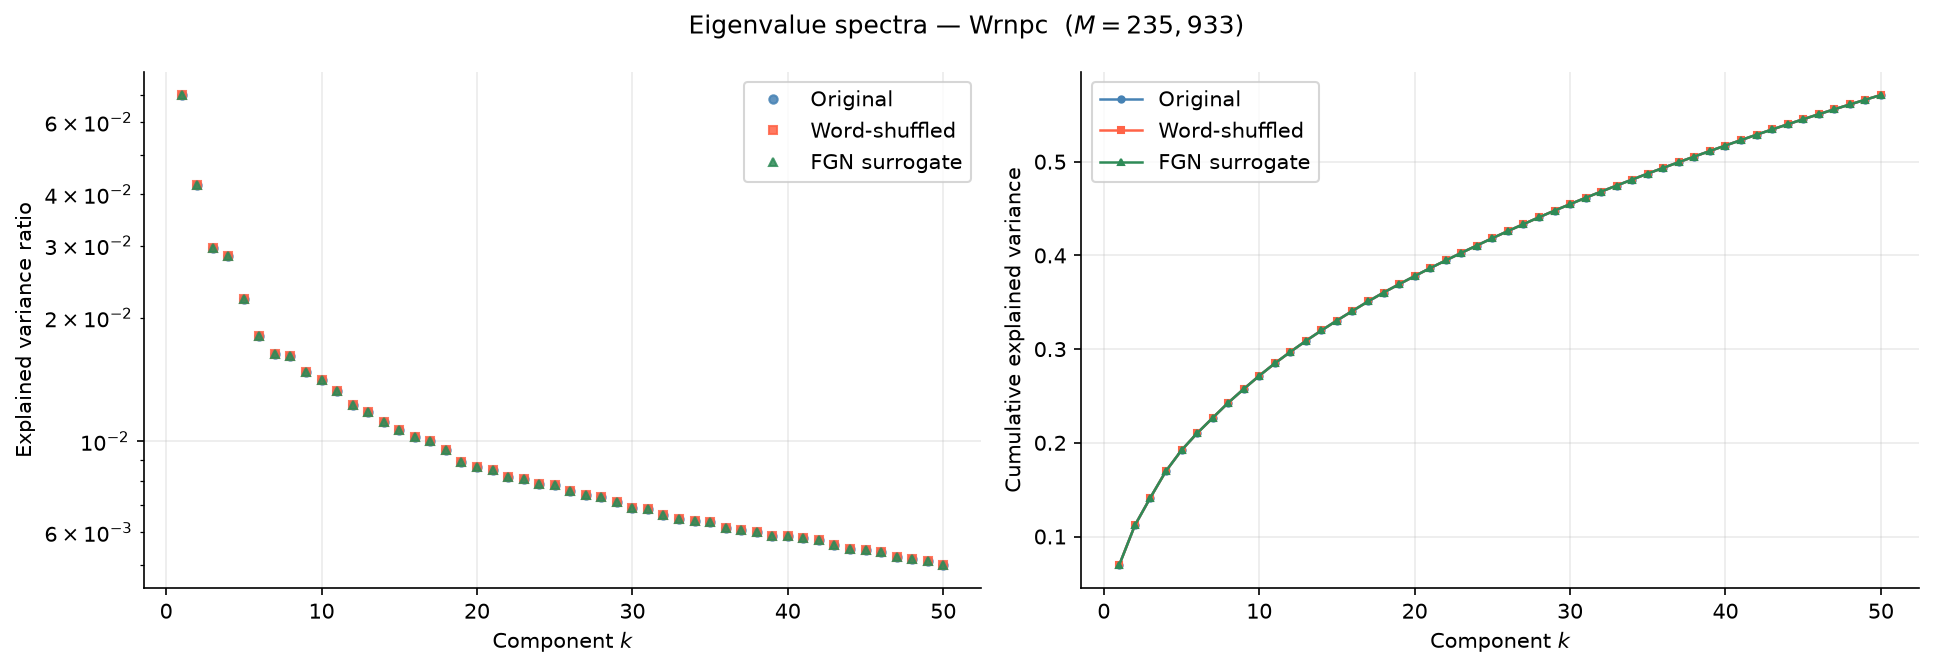
\includegraphics[width=\textwidth]{figures/eng_wrnpc/eng_wrnpc_02_spectra_comparison.png}
  \caption{Eigenvalue spectra and cumulative explained variance for
  \emph{War and Peace}: original (blue), word-shuffled (red), and
  FGN surrogate (green). The shuffled spectrum is identical to the
  original by permutation invariance; the FGN spectrum is empirically
  very close over the displayed range (Remark~\ref{rem:fgn_cov}).}
  \label{fig:wrnpc_spectra}
\end{figure}

The semantic poles in Table~\ref{tab:wrnpc_pc} reveal two especially clear contrasts. PC2
separates military vocabulary (\emph{regiment}, \emph{infantry},
\emph{cavalry}, \emph{battalion}) from personal and emotional discourse
(\emph{really}, \emph{yourself}, \emph{feel}, \emph{understand}). PC3
contrasts physical action and embodied presence with philosophical and
moral reflection. PC1 partly reflects the known GloVe artefact in which
transliterated Russian names and emotionally inflected rare words lie
at the periphery of the embedding cloud; it is retained in the spectra
but interpreted cautiously.

\begin{table}[htbp]
\centering
\caption{Top-10 word types at the positive and negative poles
of PC1, PC2, and PC3 for \emph{War and Peace} ($R=100$,
$F_{\min}=5$).
Frequencies in the filtered token sequence.}
\label{tab:wrnpc_pc}
\small
\setlength{\tabcolsep}{4pt}
\begin{tabular}{ll p{6cm} p{6cm}}
\toprule
PC & Pole & Top words (freq) & Interpretation \\
\midrule
PC1 & $+$ &
  \emph{gerasim} (26), \emph{pavlovna} (151), \emph{petya} (268),
  \emph{dmitrievna} (105), \emph{piteously} (7), \emph{irritably} (6)
  & Russian proper names + emotional adverbs (GloVe artefact) \\
PC1 & $-$ &
  \emph{any} (465), \emph{government} (63), \emph{people} (557),
  \emph{can} (631), \emph{our} (619), \emph{country} (106)
  & High-frequency function/abstract English (GloVe artefact) \\
\midrule
PC2 & $+$ &
  \emph{regiment} (226), \emph{infantry} (82), \emph{cavalry} (77),
  \emph{battalion} (44), \emph{squadron} (64), \emph{army} (663)
  & Military narrative (War) \\
PC2 & $-$ &
  \emph{really} (203), \emph{yourself} (117), \emph{feel} (133),
  \emph{myself} (148), \emph{think} (357), \emph{understand} (347)
  & Personal/emotional discourse (Peace) \\
\midrule
PC3 & $+$ &
  \emph{walked} (70), \emph{sat} (345), \emph{feet} (112),
  \emph{screaming} (6), \emph{legs} (101), \emph{bed} (118)
  & Physical action, embodied presence \\
PC3 & $-$ &
  \emph{principles} (7), \emph{obligations} (6), \emph{moral} (32),
  \emph{justification} (11), \emph{renounce} (8), \emph{unjust} (7)
  & Philosophical/moral reflection \\
\bottomrule
\end{tabular}
\end{table}

\subsubsection{\emph{On the Origin of Species}}
\label{sec:darwin}

\emph{On the Origin of Species} contains $N=151{,}179$ raw tokens and
$M=58{,}913$ retained tokens, with $\alpha=0.771$ and
$\alpha_0=0.80$. PC1 explains $6.61\%$ of the variance, PC2
$3.58\%$, and the first ten components $26.4\%$. The original,
shuffled, and FGN spectra are again closely aligned
(Figure~\ref{fig:darwin_spectra}).

PC1 is dominated by specialised nineteenth-century biological and
geological terminology at one pole and pronouns or conversational
markers at the other, and therefore contains a register-related
embedding artefact. PC2 is a substantive geographical-versus-epistemic
direction: spatial and biogeographical terms are opposed to the
language of inference and theoretical reasoning. PC3 contrasts
first-person field observations and concrete specimens with abstract
classification and synthesis. These poles are listed in Table~\ref{tab:darwin_pc}.

\begin{table}[htbp]
\centering
\caption{Top-10 word types at the positive and negative poles
of PC1, PC2, and PC3 for \emph{On the Origin of Species}
($R=100$, $F_{\min}=5$).}
\label{tab:darwin_pc}
\small
\setlength{\tabcolsep}{4pt}
\begin{tabular}{ll p{6cm} p{5.5cm}}
\toprule
PC & Pole & Top words (freq) & Interpretation \\
\midrule
PC1 & $+$ &
  \emph{sessile} (11), \emph{faunas} (14), \emph{ovules} (6),
  \emph{polymorphic} (9), \emph{insectivorous} (6),
  \emph{larvae} (26), \emph{palaeozoic} (15)
  & Specialised 19th-c.\ natural history lexicon \\
PC1 & $-$ &
  \emph{he} (163), \emph{him} (17), \emph{said} (47),
  \emph{us} (104), \emph{my} (150), \emph{who} (75)
  & Pronouns / interpersonal register (GloVe artefact) \\
\midrule
PC2 & $+$ &
  \emph{northern} (37), \emph{islands} (131), \emph{sea} (100),
  \emph{southern} (43), \emph{tropical} (16),
  \emph{archipelago} (37), \emph{coast} (18)
  & Geographical distribution chapters \\
PC2 & $-$ &
  \emph{understand} (74), \emph{infer} (31),
  \emph{necessarily} (27), \emph{plainly} (43),
  \emph{suppose} (63), \emph{ought} (40)
  & Scientific reasoning and theoretical inference \\
\midrule
PC3 & $+$ &
  \emph{beaks} (10), \emph{ants} (27), \emph{legs} (37),
  \emph{dog} (20), \emph{flowers} (61),
  \emph{beetles} (17), \emph{me} (153)
  & Field observations, specific specimens, first-person \\
PC3 & $-$ &
  \emph{geographical} (42), \emph{distribution} (55),
  \emph{proportional} (16), \emph{classification} (49),
  \emph{development} (28), \emph{fundamental} (9)
  & Abstract synthesis, quantitative generalisation \\
\bottomrule
\end{tabular}
\end{table}

\subsubsection{\emph{Great Expectations}}
\label{sec:greatexp}

\emph{Great Expectations} contains $N=188{,}925$ raw tokens and
$M=64{,}410$ retained tokens, with $\alpha=0.689$ and
$\alpha_0=0.74$. PC1, PC2, and the first ten components account for
$6.54\%$, $4.34\%$, and $27.2\%$ of the variance, respectively. The
three covariance spectra are again nearly coincident
(Figure~\ref{fig:greatexp_spectra}).

The positive pole of PC1 contains character names and Dickensian
dialect, opposed to generic vocabulary, and is treated as an embedding
artefact. PC2 contrasts spatial and kinetic language associated with
the river, marshes, and forge with introspective and conversational
language. PC3 opposes embodied physical description to legal and
institutional vocabulary, reflecting the tension between Pip's lived
world and the machinery of inheritance and social advancement. The
corresponding poles are listed in Table~\ref{tab:greatexp_pc}.

\begin{table}[htbp]
\centering
\caption{Top-10 word types at the positive and negative poles
of PC1, PC2, and PC3 for \emph{Great Expectations}
($R=100$, $F_{\min}=5$).}
\label{tab:greatexp_pc}
\small
\setlength{\tabcolsep}{4pt}
\begin{tabular}{ll p{6cm} p{5.5cm}}
\toprule
PC & Pole & Top words (freq) & Interpretation \\
\midrule
PC1 & $+$ &
  \emph{jaggers} (242), \emph{estella} (270), \emph{biddy} (231),
  \emph{provis} (70), \emph{magwitch} (26),
  \emph{limekiln} (6), \emph{tickler} (10)
  & Character names + Victorian dialect (GloVe artefact) \\
PC1 & $-$ &
  \emph{will} (174), \emph{any} (268), \emph{their} (175),
  \emph{two} (254), \emph{last} (185), \emph{other} (201)
  & High-frequency generic vocabulary \\
\midrule
PC2 & $+$ &
  \emph{river} (59), \emph{near} (66), \emph{opened} (41),
  \emph{fell} (55), \emph{port} (7), \emph{yards} (9),
  \emph{miles} (17)
  & Spatial/kinetic (Thames, marshes, forge) \\
PC2 & $-$ &
  \emph{really} (41), \emph{think} (241), \emph{myself} (235),
  \emph{understand} (53), \emph{feel} (28),
  \emph{ashamed} (15), \emph{want} (93)
  & Introspective/conversational register \\
\midrule
PC3 & $+$ &
  \emph{legs} (35), \emph{walked} (45), \emph{feet} (34),
  \emph{knees} (15), \emph{fingers} (31),
  \emph{shoulder} (54), \emph{bed} (74)
  & Physical, embodied description \\
PC3 & $-$ &
  \emph{authority} (8), \emph{constitutional} (5),
  \emph{law} (9), \emph{appointed} (11),
  \emph{established} (13), \emph{derived} (13)
  & Legal/institutional machinery \\
\bottomrule
\end{tabular}
\end{table}

\subsubsection{\emph{Ulysses}}
\label{sec:ulysses}

\emph{Ulysses} contains $N=264{,}165$ raw tokens and $M=101{,}489$
retained tokens, with $\alpha=0.763$ and $\alpha_0=0.80$. Its first
ten components account for $25.0\%$ of the variance, the smallest
fraction among the four texts, consistent with the diversity of
registers across its eighteen episodes
(Figure~\ref{fig:ulysses_spectra}).

PC1 is strongly affected by Dublin-specific proper names,
multilingual fragments, and neologisms. PC2 provides a more substantive
formal-public versus intimate-private contrast, separating titles,
institutional names, and parodic catalogue language from colloquial and
sensory interior discourse. PC3 contrasts physical-material description
with vocabulary of family, religion, and literary identity. These
semantic poles are listed in Table~\ref{tab:ulysses_pc}.

\begin{table}[htbp]
\centering
\caption{Top-10 word types at the positive and negative poles
of PC1, PC2, and PC3 for \emph{Ulysses} ($R=100$, $F_{\min}=5$).}
\label{tab:ulysses_pc}
\small
\setlength{\tabcolsep}{4pt}
\begin{tabular}{ll p{6.2cm} p{5.3cm}}
\toprule
PC & Pole & Top words (freq) & Interpretation \\
\midrule
PC1 & $+$ &
  \emph{dedalus} (174), \emph{dignam} (83),
  \emph{lenehan} (107), \emph{gerty} (64),
  \emph{virag} (43), \emph{voglio} (9)
  & Dublin proper names + multilingual fragments (GloVe artefact) \\
PC1 & $-$ &
  \emph{government} (14), \emph{people} (78),
  \emph{country} (54), \emph{world} (155),
  \emph{united} (10), \emph{china} (9)
  & Abstract political vocabulary (GloVe artefact) \\
\midrule
PC2 & $+$ &
  \emph{sir} (219), \emph{william} (40), \emph{john} (196),
  \emph{royal} (47), \emph{edward} (17),
  \emph{founded} (8), \emph{lieutenant} (13)
  & Formal titles, institutional names, parodic chapters \\
PC2 & $-$ &
  \emph{yourself} (38), \emph{feel} (104),
  \emph{myself} (71), \emph{really} (49),
  \emph{laugh} (37), \emph{smell} (50), \emph{awfully} (22)
  & Intimate register, internal monologue episodes \\
\midrule
PC3 & $+$ &
  \emph{thick} (26), \emph{surface} (10), \emph{mud} (6),
  \emph{feet} (82), \emph{yellow} (50),
  \emph{sand} (32), \emph{shells} (14)
  & Physical-material description (Sandymount Strand, streets) \\
PC3 & $-$ &
  \emph{married} (56), \emph{son} (113), \emph{wife} (140),
  \emph{brother} (66), \emph{god} (247),
  \emph{dear} (83), \emph{friend} (68)
  & Family, religion, literary identity (Telemachus, Nostos) \\
\bottomrule
\end{tabular}
\end{table}

Taken together, the four texts show that PCA produces an ordered static
geometry whose leading directions are often semantically interpretable,
but whose first component can be contaminated by peripheral lexical
clusters. The temporal question is separate: whether visits along these
directions occur regularly or in concentrated textual episodes.

\FloatBarrier
\subsection{Burstiness across principal components}
\label{sec:component_burstiness_results}

We now turn from static geometry to temporal organisation. For each
component, threshold crossings define event sequences and IET
distributions. Figure~\ref{fig:burst_panel} and
Figures~\ref{fig:wrnpc_iet}, \ref{fig:darwin_iet}, \ref{fig:greatexp_iet}
and \ref{fig:ulysses_iet} show the representative-text evidence. In every text, the original
series has broader IET distributions and larger $B_k$ than either
control. The spectra are component dependent and generally largest
among the early PCs, but the decay with component rank is not monotone.
This non-monotonicity is expected because PCA orders variance rather
than burstiness.

\subsubsection{\emph{War and Peace}}

For PC1--PC3, the original IET distributions extend well beyond the
geometric reference, whereas the shuffled and FGN controls closely
follow it (Figure~\ref{fig:wrnpc_iet}). The burstiness spectrum in
Figure~\ref{fig:burst_panel}A is above both controls for all 20
components. PC3 has the largest value, $B_3=2.045$, approximately
$2.1$ times the geometric baseline and more than twice the corresponding
null values ($B_3^{\rm surr}=0.976$,
$B_3^{\rm FGN}=0.974$). This is consistent with the concentration of
philosophical-reflection passages in particular parts of the novel.
The eigenvalue--burstiness correlation is positive but imperfect,
$r=0.702$ ($p=0.0006$).

\begin{figure}[htbp]
  \centering
  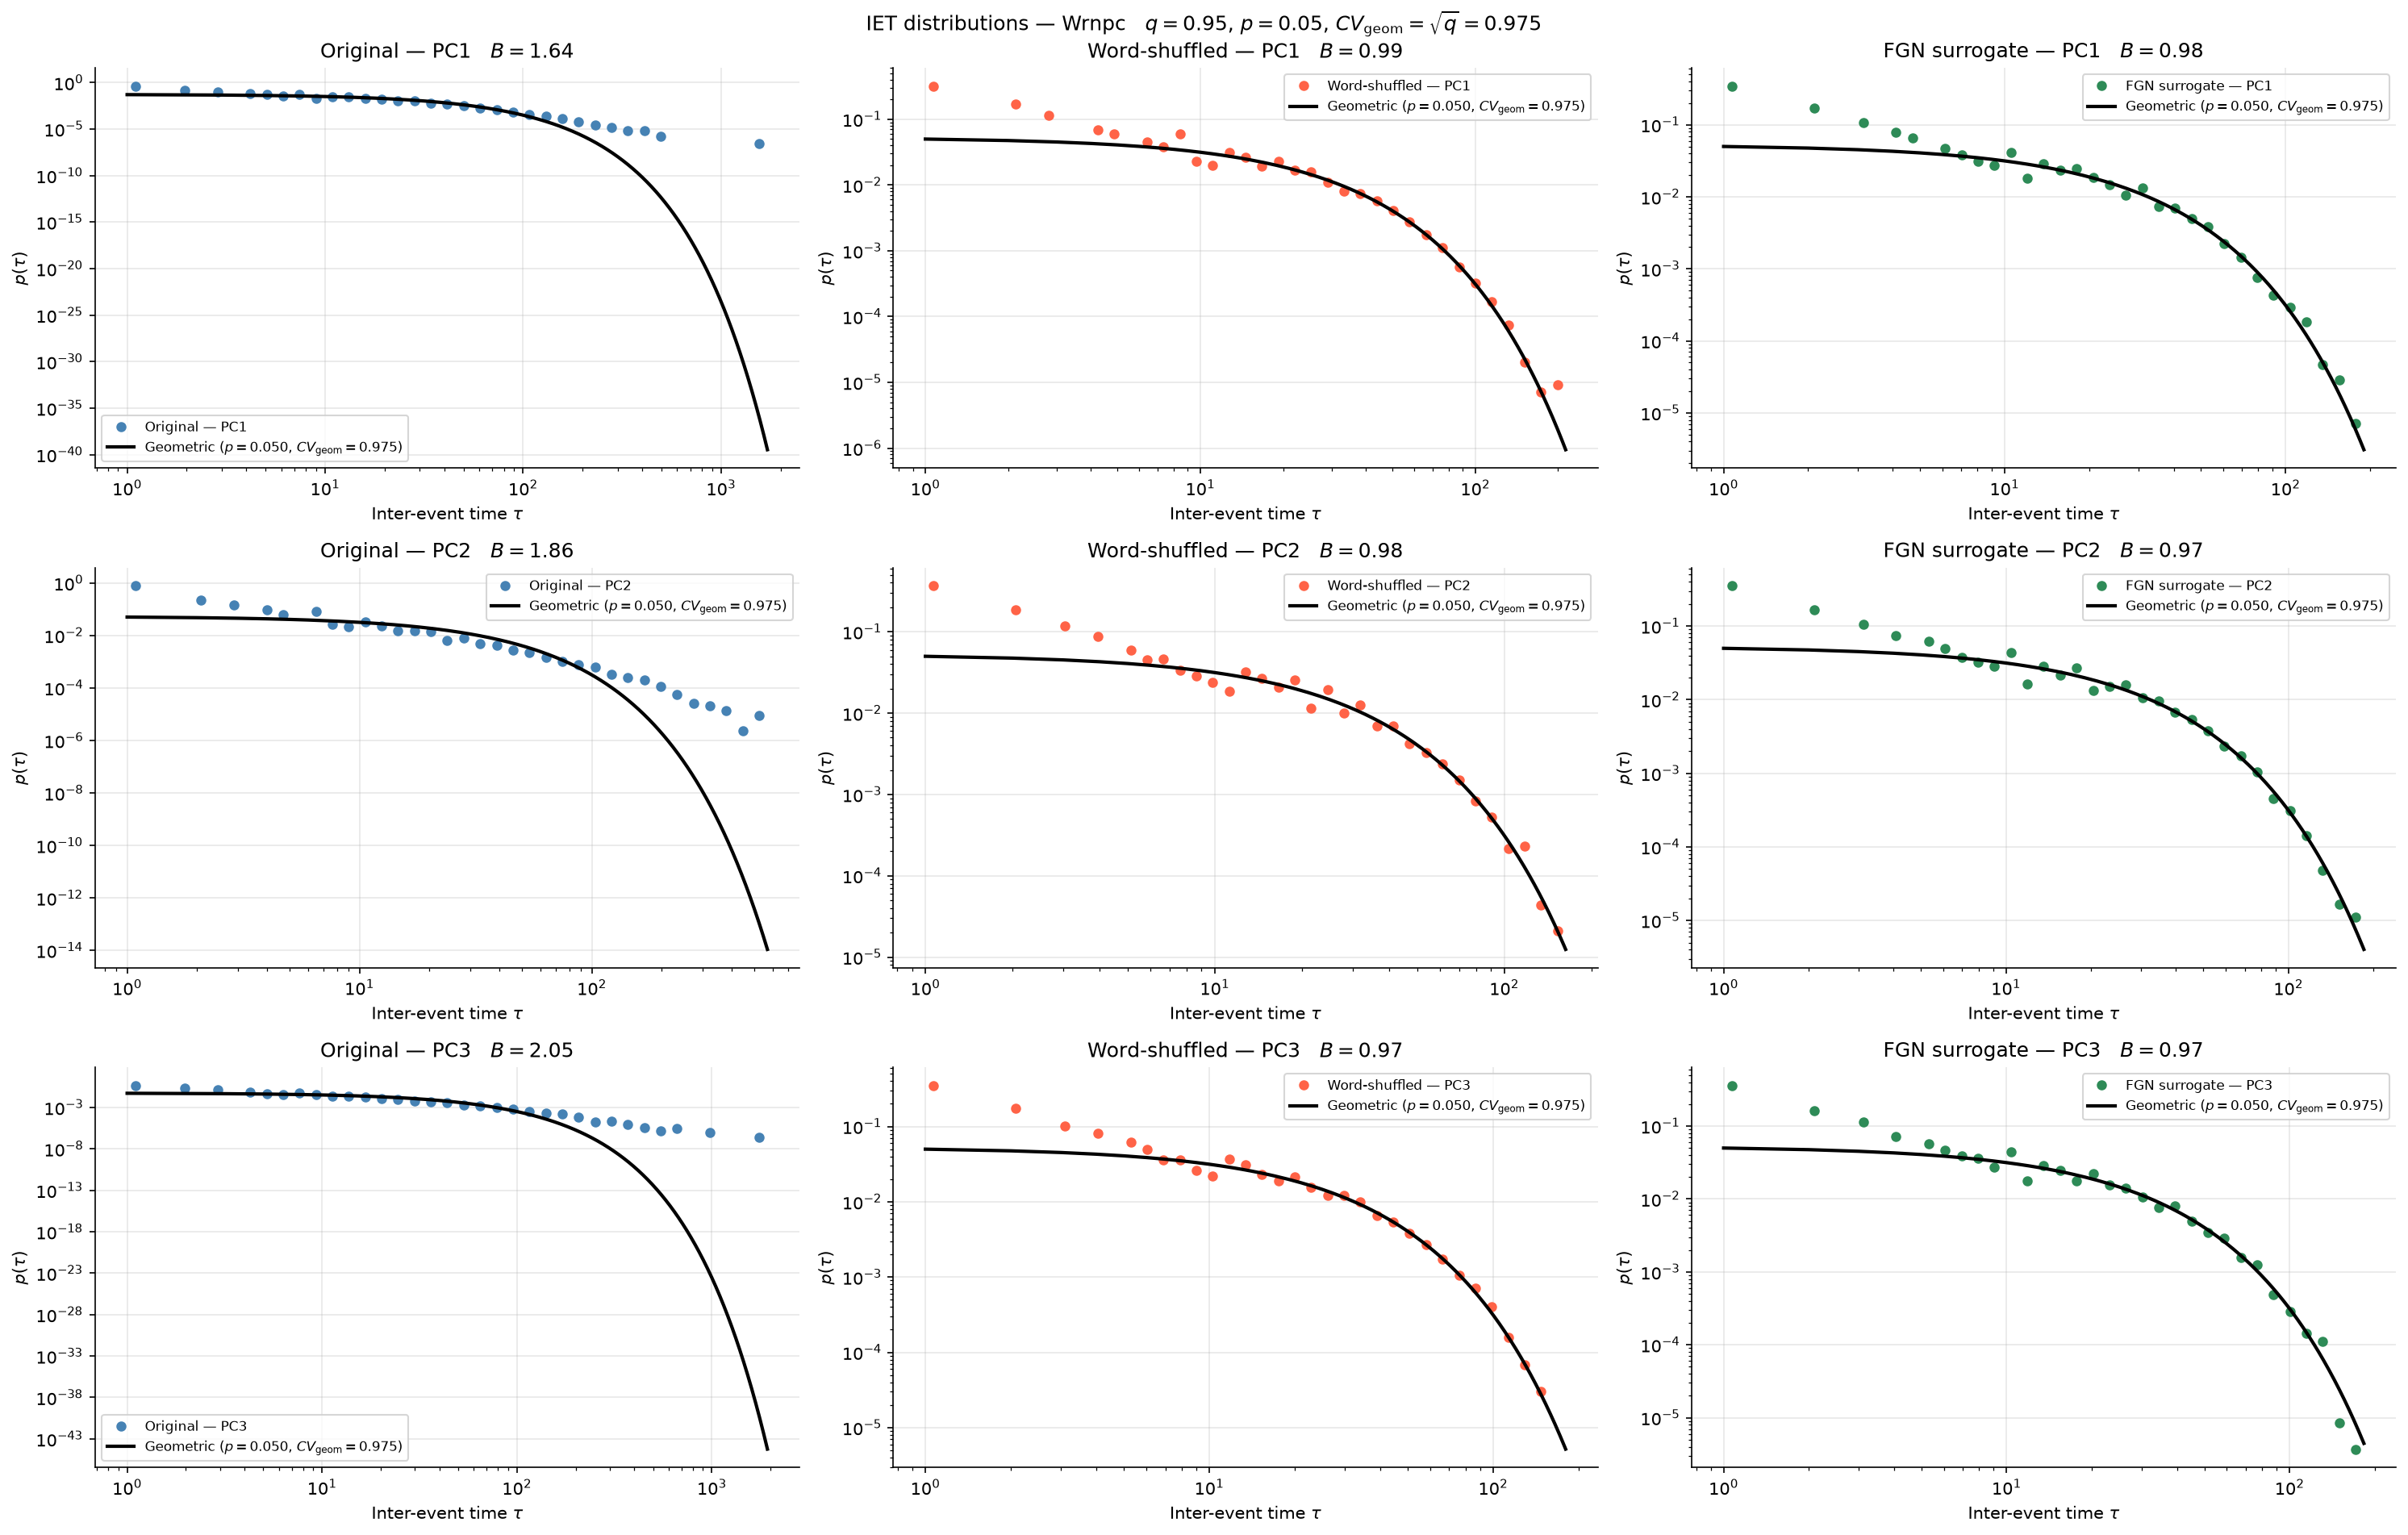
\includegraphics[width=\textwidth]{figures/eng_wrnpc/eng_wrnpc_03_iet_comparison.png}
  \caption{Inter-event-time distributions for PC1--PC3 of
  \emph{War and Peace} at $q=0.95$. Columns show the original text
  (blue), word-shuffled null (red), and FGN surrogate (green). The
  original projections have broad tails, whereas both controls lie
  close to the geometric reference.}
  \label{fig:wrnpc_iet}
\end{figure}

\begin{figure}[htbp]
  \centering
  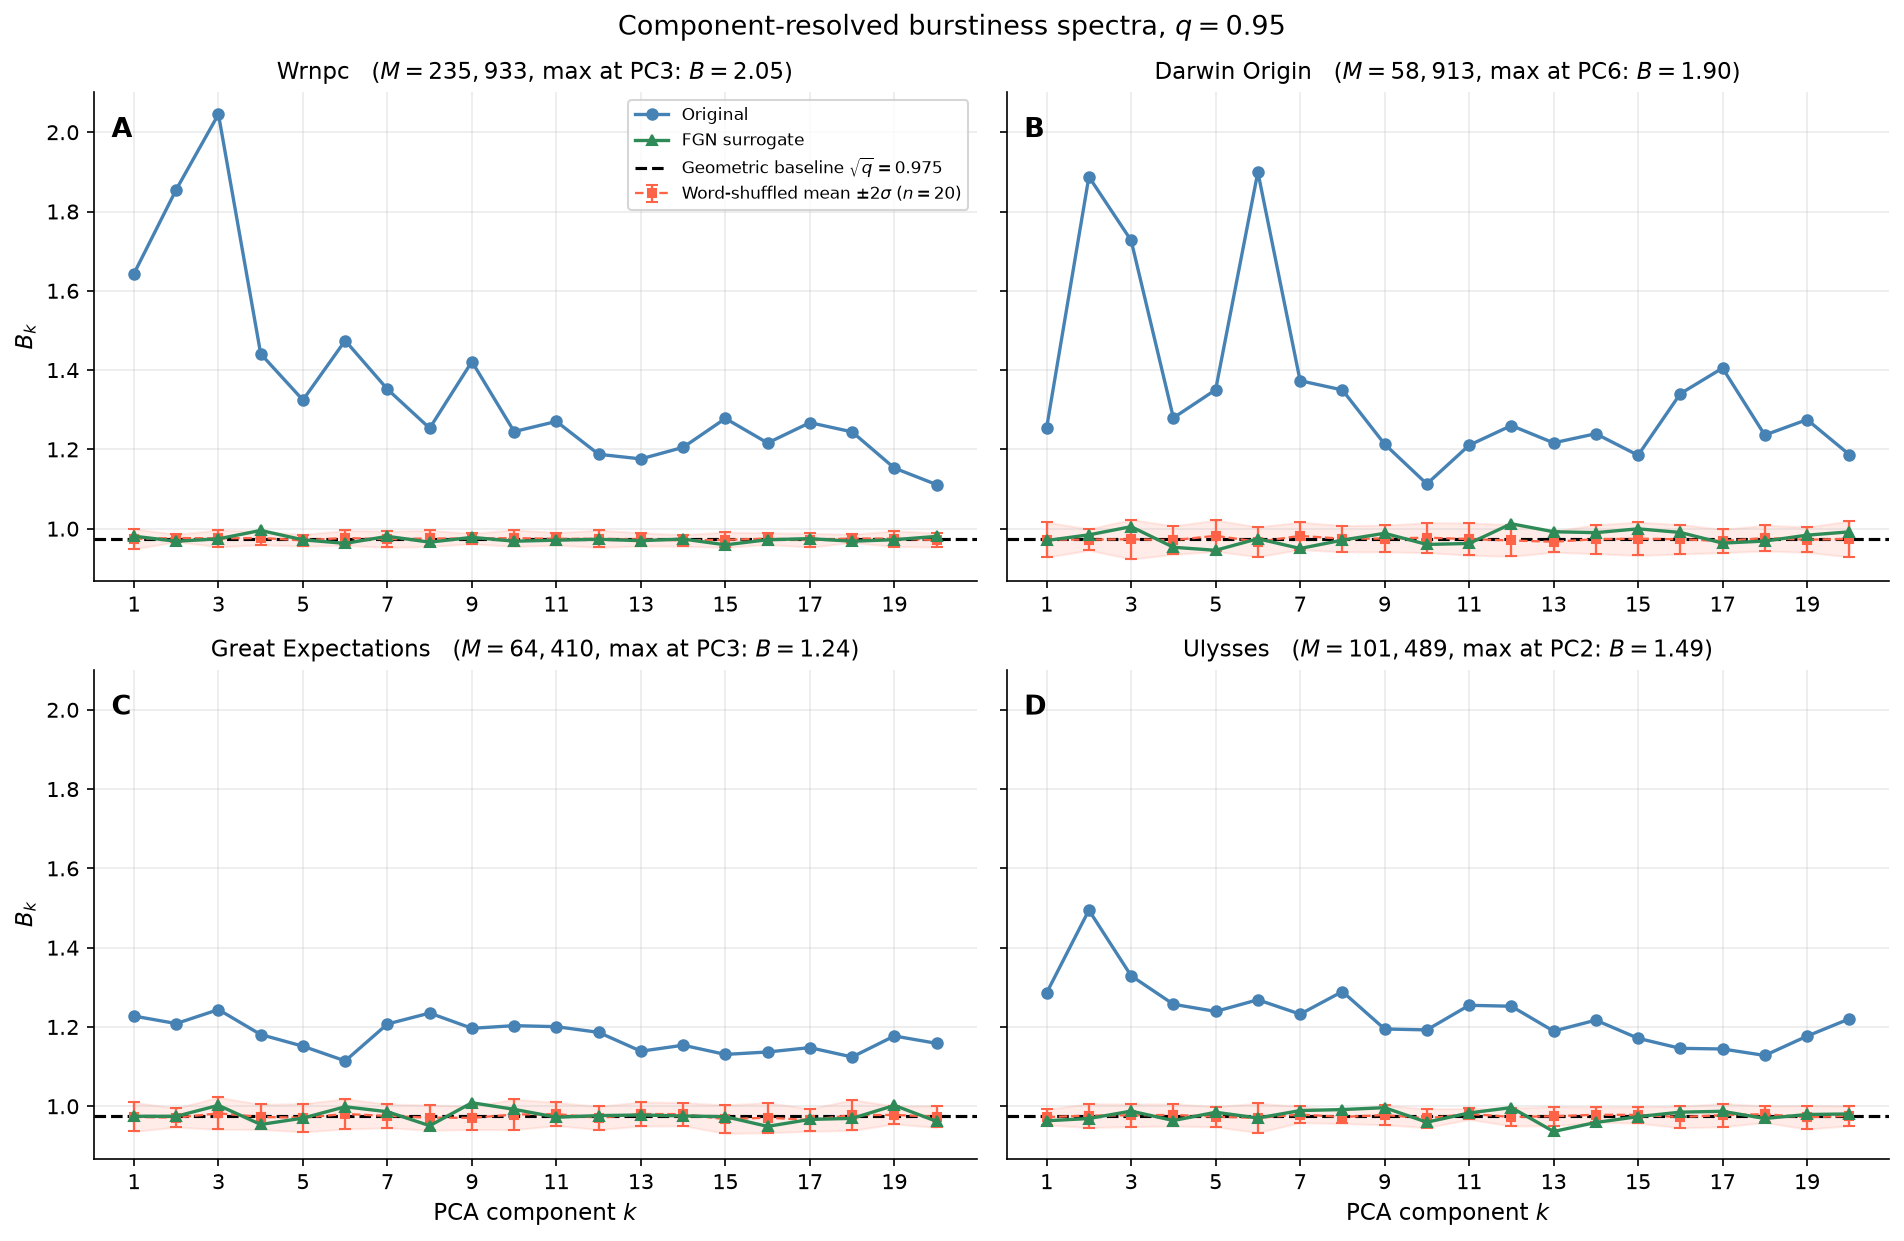
\includegraphics[width=\textwidth]{figures/panel_burstiness_spectra.png}
  \caption{Component-resolved burstiness spectra at $q=0.95$ for the four
  representative texts: \textbf{A} \emph{War and Peace},
  \textbf{B} \emph{On the Origin of Species},
  \textbf{C} \emph{Great Expectations}, \textbf{D} \emph{Ulysses}.
  In every panel the original (blue circles) lies above the FGN surrogate
  (green triangles), the word-shuffled mean$\pm2\sigma$ band (red), and the
  geometric baseline $\sqrt{q}\simeq0.975$, for all 20 components.
  The position of the maximum differs between texts (PC3, PC6, PC3 and PC2
  respectively) and burstiness is not monotone in PCA rank, because PCA
  orders components by variance rather than by temporal clustering.}
  \label{fig:burst_panel}
\end{figure}

\subsubsection{\emph{On the Origin of Species}}

The original projections have broad IET tails, particularly for PC2
and PC3, while both controls remain close to geometric
(Figure~\ref{fig:darwin_iet}). PC2 is the burstiest direction,
$B_2=1.888$, followed by PC3 with $B_3=1.727$; PC1 is lower at
$B_1=1.255$. The full original-over-control ordering holds for all 20
components. The weak eigenvalue--burstiness correlation,
$r=0.295$ ($p=0.207$), shows especially clearly that the direction of
greatest semantic variance need not be the direction of greatest
temporal clustering.

\subsubsection{\emph{Great Expectations}}

The original PC1--PC3 IET distributions again have broader tails than
the controls (Figure~\ref{fig:greatexp_iet}). At $q=0.95$,
$B_1=1.228$, $B_2=1.209$, and $B_3=1.244$, while the null values lie
in $0.95$--$1.00$. The original remains above both controls over all
20 components (Figure~\ref{fig:burst_panel}C); the spectrum is flatter
and lower overall than for \emph{War and Peace}. The correlation
between eigenvalue and burstiness is $r=0.511$ ($p=0.021$).

\subsubsection{\emph{Ulysses}}

For \emph{Ulysses}, the original IET distributions are broad for all
three displayed components, while both controls collapse towards the
geometric reference (Figure~\ref{fig:ulysses_iet}). The spectrum peaks
at PC2, $B_2=1.495$, with $B_1=1.290$ and $B_3=1.329$
(Figure~\ref{fig:burst_panel}D). The original exceeds both controls
throughout the first 20 components, and the eigenvalue--burstiness
correlation is $r=0.571$ ($p=0.009$).

Averaged over the first 20 components at $q=0.95$, the representative
texts have $\bar B^{\rm orig}$ of $1.36$ (\emph{War and Peace}),
$1.35$ (\emph{On the Origin of Species}), $1.23$ (\emph{Ulysses}) and
$1.18$ (\emph{Great Expectations}), against $\bar B\simeq0.97$--$0.98$
for both null models in every case. The ordering is not a simple
function of either text length or rank-sequence DFA exponent.
The common feature is that component-level burstiness is present in the
original semantic trajectories and absent from both null models.

\FloatBarrier
\subsection{Robustness to the threshold quantile}
\label{sec:single_text_robustness}

The component separation is not tied to the default $q=0.95$.
Figure~\ref{fig:sweep_panel} shows the mean
burstiness over $k=1,\ldots,20$ as $q$ varies from $0.60$ to $0.99$;
the corpus-level version of the ordering fraction is given in
Section~\ref{sec:corpus_robustness}.
For each of the four representative texts, the ordering holds for all
20 components throughout the displayed range. As expected, the
absolute burstiness increases towards more extreme thresholds because
rare visits to the upper tail accentuate episode-to-episode clustering.

\begin{figure}[htbp]
  \centering
  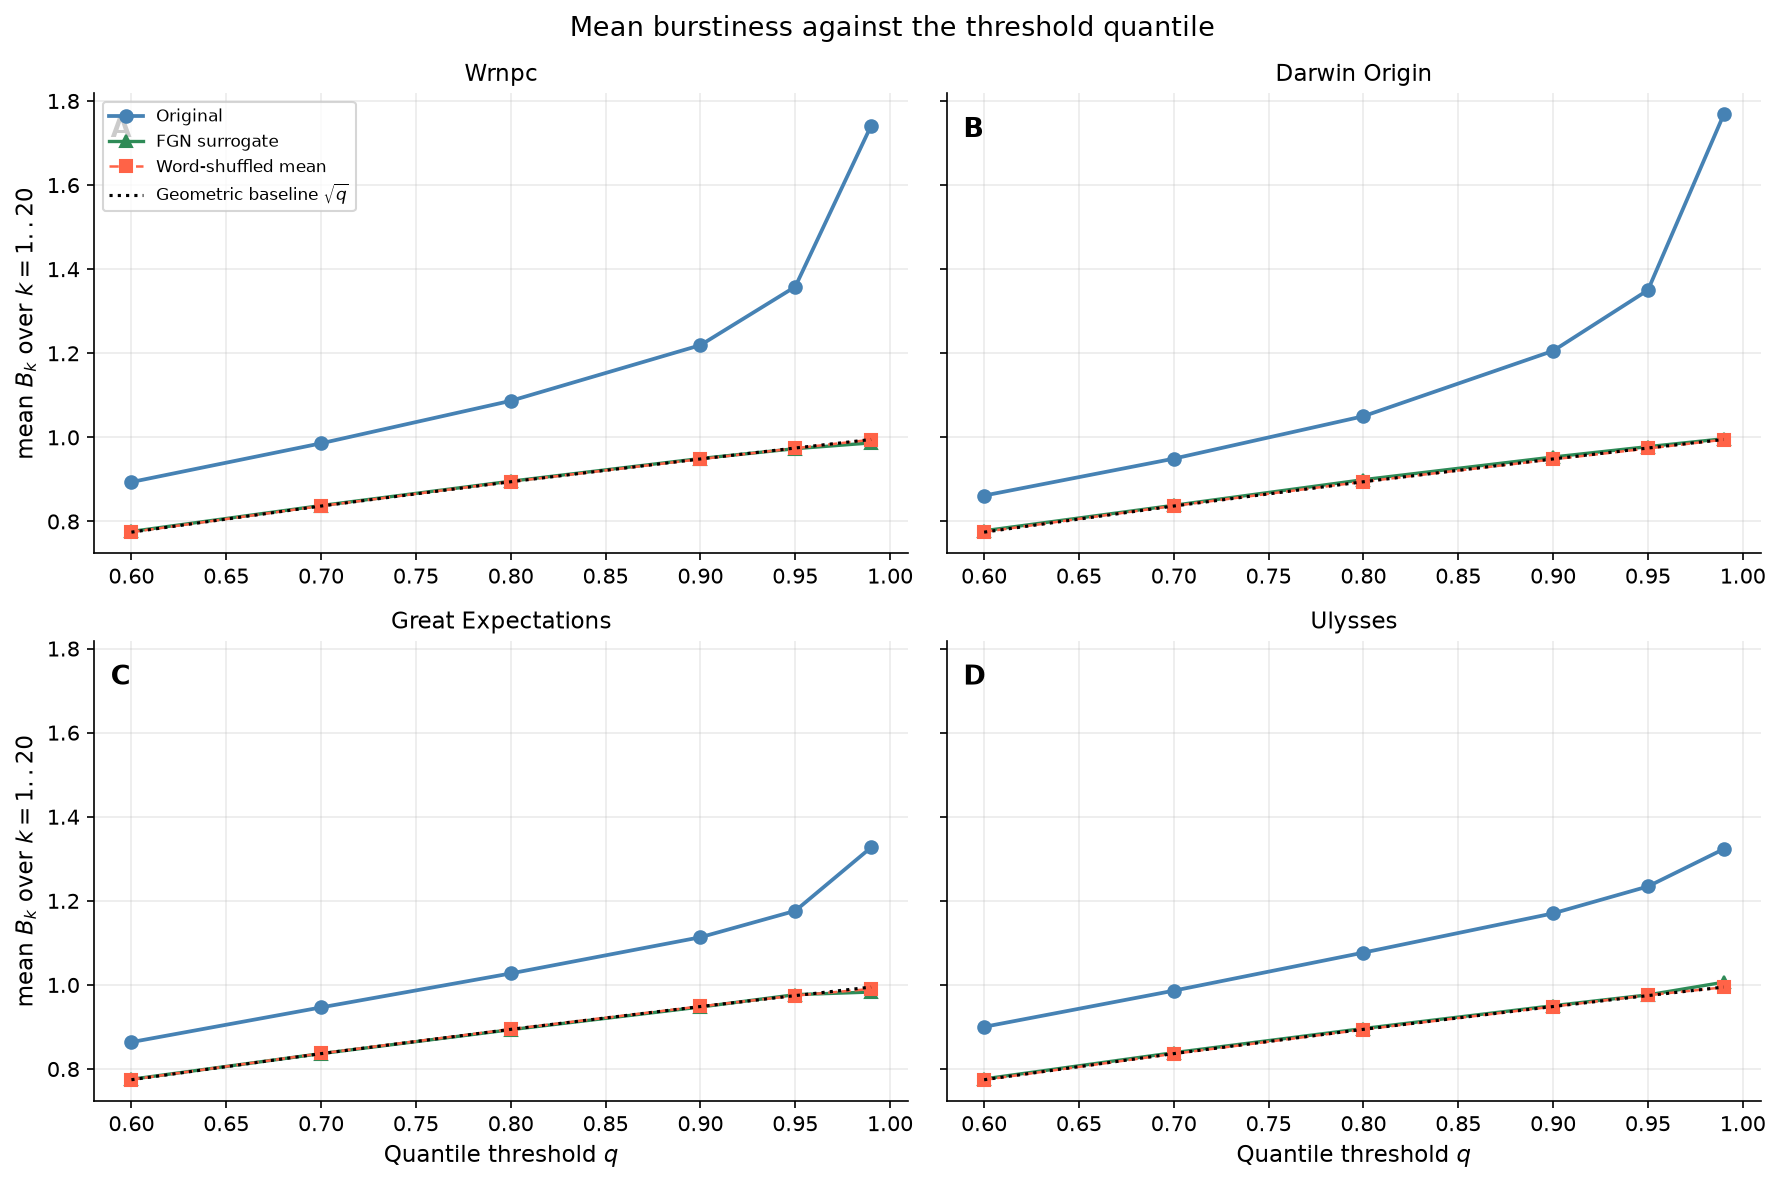
\includegraphics[width=\textwidth]{figures/panel_quantile_sweep.png}
  \caption{Mean burstiness over $k=1,\ldots,20$ as a function of the
  threshold quantile $q$, for the four representative texts:
  \textbf{A} \emph{War and Peace}, \textbf{B} \emph{On the Origin of
  Species}, \textbf{C} \emph{Great Expectations}, \textbf{D}
  \emph{Ulysses}. The original stays above both controls and above the
  geometric baseline $\sqrt{q}$ throughout $q \in [0.60, 0.99]$, and the
  full ordering $B_k^{\rm orig} > B_k^{\rm FGN}$ and
  $B_k^{\rm orig} > B_k^{\rm surr}$ holds for all 20 components at every
  displayed $q$ in each text. Absolute burstiness grows towards more
  extreme thresholds, as rare visits to the upper tail accentuate
  episode-to-episode clustering.}
  \label{fig:sweep_panel}
\end{figure}

\FloatBarrier
\section{Corpus-level generalisation}
\label{sec:corpus}

Having established the component-resolved pattern in four
representative texts (Section~\ref{sec:oliver}), we now assess its
generality across the full corpus.
%
%\NOTE{All computations use local PCA (eigenvectors re-estimated per
%text), GloVe-300 embeddings, frequency filter $R=100$, hapax filter
%$F_{\min}=5$, $N_{\rm surr}=10$ word-shuffled realisations,
%and a single FGN realisation per text (seed 42).
%Default quantile $q=0.95$ unless stated.}

\subsection{Corpus description}
\label{sec:corpus_texts}

The corpus comprises 16 English literary texts from Project Gutenberg,
spanning novels, scientific treatises, and travel writing published
between the eighteenth and early twentieth centuries
(Table~\ref{tab:corpus}).
Raw token counts range from approximately $56{,}000$ (The Picture of
Dorian Gray) to $565{,}000$ (War and Peace), with filtered token counts
$M$ (after high-frequency and hapax removal, OOV excluded) between
$17{,}000$ and $236{,}000$.
DFA scaling exponents $\alpha$ lie in the range $[0.63, 0.85]$,
consistent with the literature on long-range correlations in English
texts \citep{Ebeling1995, MontemurroPury2002}.


\begin{table}[t]
\centering
\caption{Corpus of 16 literary and scientific texts.
$N$: total token count after tokenisation.
$M$: content tokens after frequency filtering
(top $R=100$ words removed, minimum frequency~5).
$\alpha$: DFA scaling exponent of the rank sequence.
$\alpha_0$: FGN generator exponent matched to $\alpha$ (bisection
tolerance $0.01$).}
\label{tab:corpus}
\small
\begin{tabular}{llrrll}
\toprule
Title & Author & $N$ & $M$ & $\alpha$ & $\alpha_0$ \\
\midrule
Pride and Prejudice        & Austen    & 122{,}226 &  42{,}364 & 0.642 & 0.67 \\
Don Quixote (transl.)      & Cervantes & 403{,}152 & 147{,}279 & 0.711 & 0.76 \\
On the Origin of Species   & Darwin    & 151{,}179 &  58{,}913 & 0.771 & 0.80 \\
The Voyage of the Beagle   & Darwin    & 206{,}728 &  84{,}931 & 0.629 & 0.67 \\
David Copperfield          & Dickens   & 363{,}557 & 134{,}409 & 0.727 & 0.78 \\
Great Expectations         & Dickens   & 188{,}925 &  64{,}410 & 0.689 & 0.74 \\
Oliver Twist               & Dickens   & 161{,}529 &  59{,}729 & 0.711 & 0.76 \\
Ulysses                    & Joyce     & 264{,}165 & 101{,}489 & 0.763 & 0.80 \\
The Jungle Book            & Kipling   & 151{,}161 &  49{,}522 & 0.775 & 0.83 \\
Moby Dick                  & Melville  & 215{,}652 &  82{,}773 & 0.694 & 0.73 \\
Principia Mathematica      & Newton    & 112{,}225 &  26{,}347 & 0.815 & 0.85 \\
The Analysis of Mind       & Russell   &  88{,}342 &  30{,}449 & 0.743 & 0.76 \\
War and Peace              & Tolstoy   & 564{,}788 & 235{,}933 & 0.721 & 0.76 \\
Huckleberry Finn           & Twain     & 145{,}924 &  52{,}741 & 0.774 & 0.83 \\
Tom Sawyer                 & Twain     &  71{,}102 &  22{,}085 & 0.788 & 0.80 \\
The Picture of Dorian Gray & Wilde     &  55{,}619 &  16{,}776 & 0.845 & 0.87 \\
\bottomrule
\end{tabular}
\end{table}

\begin{quote}
Per-text IET distributions and burstiness spectra for all texts and
threshold values can be regenerated with \texttt{scripts/run\_text.py}
in the code repository. The main text reports the aggregated corpus
results.
\end{quote}


% ??????????????????????????????????????????????????????????
% Corpus ordering subsections ? rewritten
% ??????????????????????????????????????????????????????????

\subsection{Component-resolved burstiness holds corpus-wide}
\label{sec:corpus_ordering}

The corpus-level component spectrum is summarised in
Figure~\ref{fig:corpus_spectrum}.
Averaging the burstiness spectrum $\{\bk\}$ across all 16 texts
at quantile $q = 0.95$, the original texts are systematically more
bursty than both null models across all 20 PCA components:
$\langle B_k^{\rm orig}\rangle_{\rm texts} \in [1.16, 1.54]$
(mean $1.26$), while both null models cluster tightly around
the geometric baseline $\CV_{\rm geom} = \sqrt{0.95} \approx 0.975$:
$\langle B_k^{\rm surr}\rangle \in [0.973, 0.978]$ and
$\langle B_k^{\rm FGN}\rangle \in [0.958, 0.983]$.

At the level of individual $({\rm text}, k)$ pairs
($16 \times 20 = 320$ pairs):
\begin{itemize}
  \item $B_k^{\rm orig} > B_k^{\rm surr}$ in $\mathbf{100\%}$ of pairs.
  \item $B_k^{\rm orig} > B_k^{\rm FGN}$ in $\mathbf{100\%}$ of pairs.
  \item $|B_k^{\rm FGN}/B_k^{\rm surr} - 1| < 0.05$ in
        $\mathbf{95.6\%}$ of pairs.
\end{itemize}

The appropriate summary statistic for the magnitude of the effect
is the \emph{per-text mean ratio}, computed by averaging
$B_k^{\rm orig}/B_k^{\rm surr}$ over the 20 components for each
text and then averaging over the 16 texts:
\begin{equation}
  \left\langle \frac{B_k^{\rm orig}}{B_k^{\rm surr}}
  \right\rangle_{\rm texts}
  \;=\; 1.29 \;\pm\; 0.03,
  \qquad t = 8.7,\quad p < 10^{-6},
  \label{eq:ratio_corpus}
\end{equation}
where $\pm$ denotes the standard error of the mean over 16 texts.
The original texts are thus on average $\sim 30\%$ more bursty
than the geometric null. The per-text values range from $1.17$
(\emph{Pride and Prejudice}) to $1.39$ (\emph{War and Peace}) for
fifteen of the sixteen texts, with \emph{Principia Mathematica} as
an outlier at $1.73$; the spread across texts (sd $= 0.13$) is
itself a signature of how differently topical structure is organised
in different works.
The analogous ratio for the FGN surrogate is
$\langle B_k^{\rm orig}/B_k^{\rm FGN}\rangle = 1.29 \pm 0.03$,
indistinguishable from the word-shuffled value.

The two null models satisfy
$\langle B_k^{\rm FGN}/B_k^{\rm surr}\rangle = 1.001 \pm 0.001$
(range over texts $[0.996, 1.005]$; $t = 1.1$, $p = 0.28$):
the FGN surrogate and the word-shuffled null are statistically
indistinguishable at the corpus level
(Section~\ref{sec:corpus_diffs}).

\begin{figure}[htbp]
  \centering
  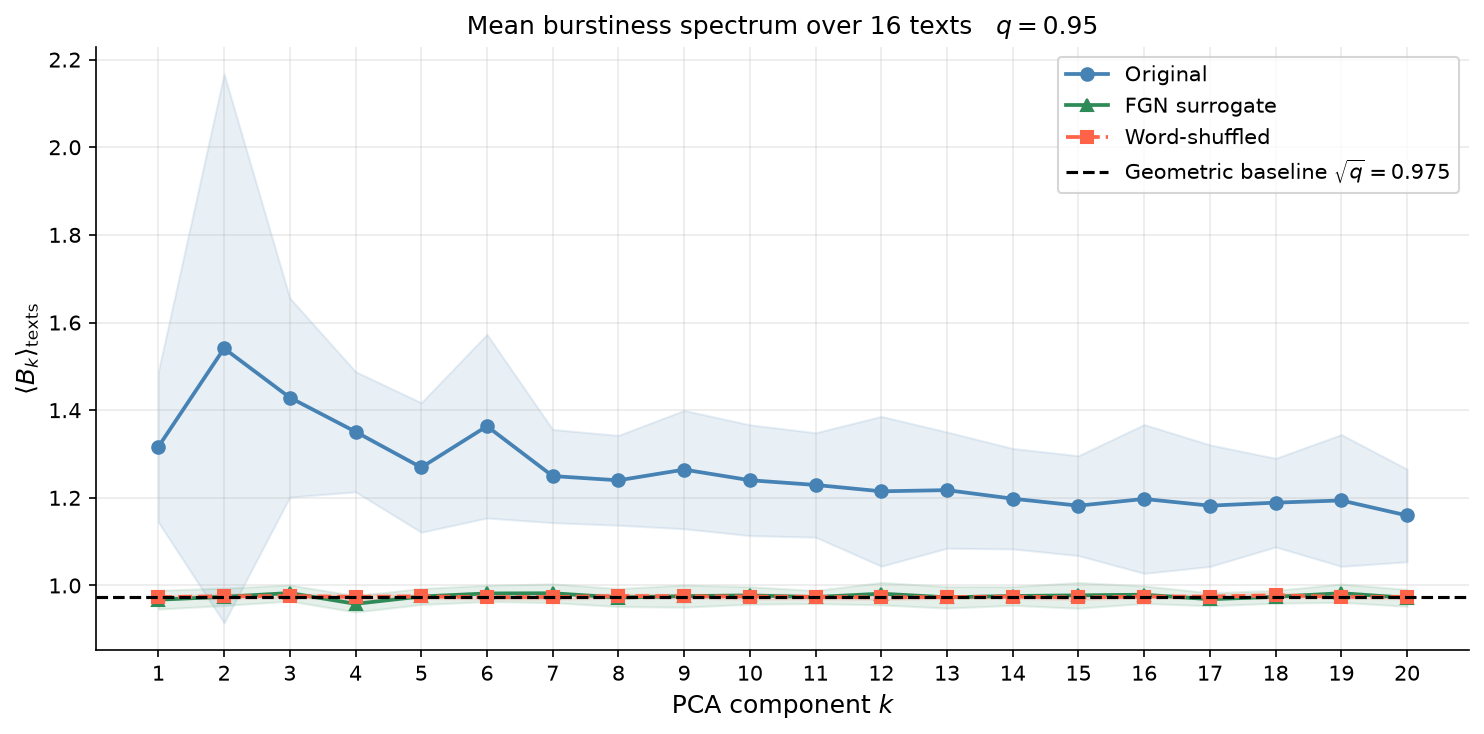
\includegraphics[width=\textwidth]{figures/fig1_mean_spectrum.png}
  \caption{Mean component-resolved burstiness spectrum across the
  analysed corpus at $q=0.95$. Curves show the mean $\langle B_k\rangle$
  over texts for $k=1,\ldots,20$; shaded bands indicate one standard
  deviation. The original texts (blue) are above the FGN surrogate
  (green), word-shuffled null (red), and geometric baseline
  $\sqrt{q}\simeq0.975$ at every component. The largest corpus means
  occur among the early components, followed by a broad decline with
  non-monotone secondary peaks.}
  \label{fig:corpus_spectrum}
\end{figure}


\subsection{Robustness across quantile threshold}
\label{sec:corpus_robustness}

Figure~\ref{fig:corpus_robustness} shows the fraction of
$({\rm text}, k)$ pairs satisfying the ordering conditions as a
function of $q \in \{0.60, 0.70, 0.80, 0.90, 0.95, 0.99\}$.

The full ordering $B_k^{\rm orig} > B_k^{\rm surr}$ and
$B_k^{\rm orig} > B_k^{\rm FGN}$ is satisfied in $100\%$
of pairs for all $q \in [0.60, 0.95]$, and in $98.1\%$ of pairs at the
extreme $q = 0.99$.
The null-model indistinguishability criterion
$|B_k^{\rm FGN}/B_k^{\rm surr} - 1| < 0.05$ is met by $\geq 99\%$ of
pairs for $q \leq 0.90$, by $96\%$ at $q = 0.95$, and decreases to
$73\%$ at $q = 0.99$.
This degradation at the extreme threshold is expected: with
$p = 0.01$ and $M \approx 80{,}000$ filtered tokens, there are
on average only $\sim 800$ events per series, giving an IET
estimator with relative error $\sim 1/\sqrt{800} \approx 3.5\%$
--- comparable to the magnitude of $B^{\rm FGN} - B^{\rm surr}$
at this threshold, and larger still for the shortest texts
($M < 30{,}000$).
For $q = 0.95$ ($n_{\rm events} \approx 4{,}000$, relative error
$\sim 1.6\%$), the estimator is well within the regime where the
null-model comparison is reliable.

\begin{figure}[htbp]
  \centering
  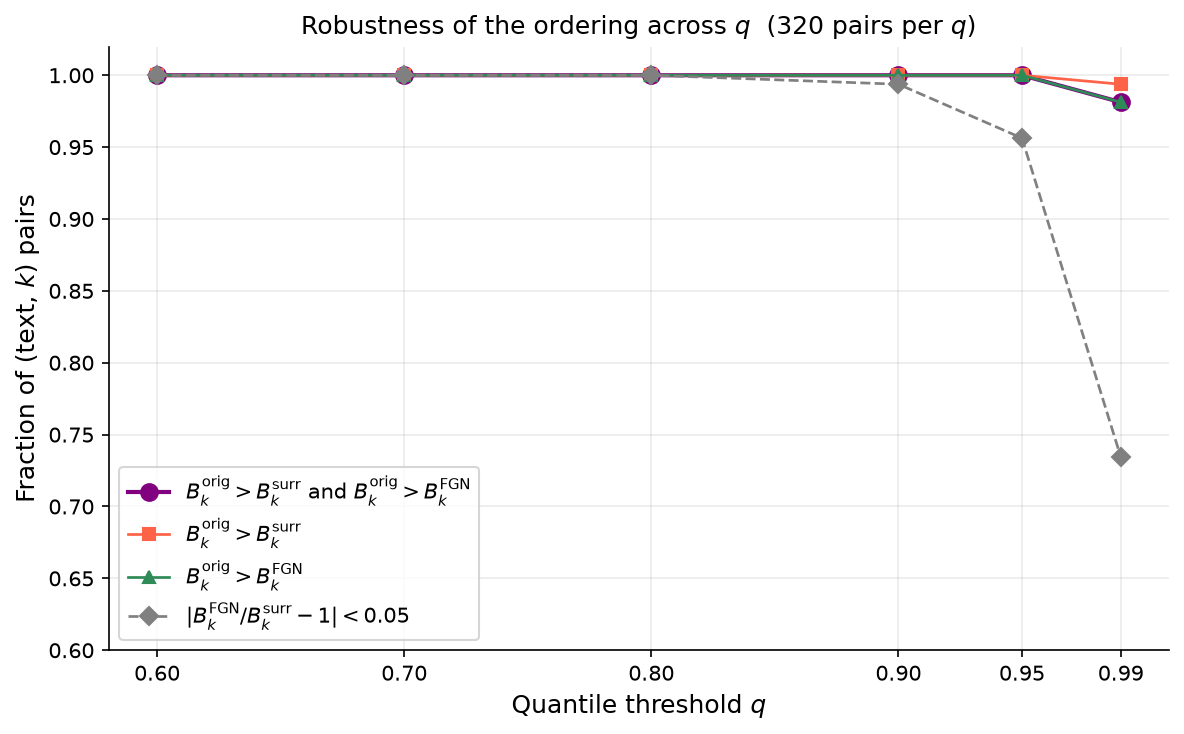
\includegraphics[width=0.72\textwidth]{figures/fig2_robustness_vs_q.png}
  \caption{%
    \textbf{Robustness of the burstiness ordering across quantile
    threshold $q$.}
    Each point: fraction of $({\rm text}, k)$ pairs ($320$ per $q$)
    satisfying the indicated condition.
    Purple circles: full ordering
    $B_k^{\rm orig} > B_k^{\rm surr}$ and $B_k^{\rm orig} >
    B_k^{\rm FGN}$.
    Red squares: $B_k^{\rm orig} > B_k^{\rm surr}$.
    Green triangles: $B_k^{\rm orig} > B_k^{\rm FGN}$.
    Grey diamonds: $|B_k^{\rm FGN}/B_k^{\rm surr} - 1| < 0.05$.
    The ordering is robust for $q \in [0.60, 0.95]$; the slight
    degradation at $q = 0.99$ is due to estimator noise at
    $p = 0.01$.
  }
  \label{fig:corpus_robustness}
\end{figure}


\subsection{Distribution of burstiness ratios}
\label{sec:corpus_diffs}

Figure~\ref{fig:corpus_diffs} shows the distribution of the ratios
$B^{\rm orig}/B^{\rm surr}$, $B^{\rm orig}/B^{\rm FGN}$, and
$B^{\rm FGN}/B^{\rm surr}$ over all 320 $({\rm text}, k)$ pairs
at $q = 0.95$.

Panel~A shows that both orig--null ratios are concentrated
well above 1, with virtually no mass below 1.
The two distributions (orig/surr and orig/FGN) are nearly
identical in shape and location, confirming that the FGN and
word-shuffled null models are equally poor surrogates for the
original burstiness.

Panel~B isolates the ratio $B^{\rm FGN}/B^{\rm surr}$, which
is tightly concentrated around 1 (mean $1.0008$, s.e.\ $0.0012$,
range $[0.91, 1.09]$).
A one-sample $t$-test against ratio\,=\,1 gives $t = 0.63$,
$p = 0.53$: the two null models are statistically indistinguishable,
and the distribution is symmetric with no indication of a
directional bias.

Together, Figures~\ref{fig:corpus_spectrum}--\ref{fig:corpus_diffs}
establish the corpus-level result:
\begin{equation}
  B_k^{\rm orig} \;\gg\; B_k^{\rm FGN} \;\approx\; B_k^{\rm surr}
  \qquad \forall\, k,\; \forall\, \text{text in corpus},
  \label{eq:ordering_corpus}
\end{equation}
with a $\sim 30\%$ mean excess of the original above the
geometric null, independent of text length, genre, DFA exponent,
and choice of quantile threshold.

\begin{figure}[htbp]
  \centering
  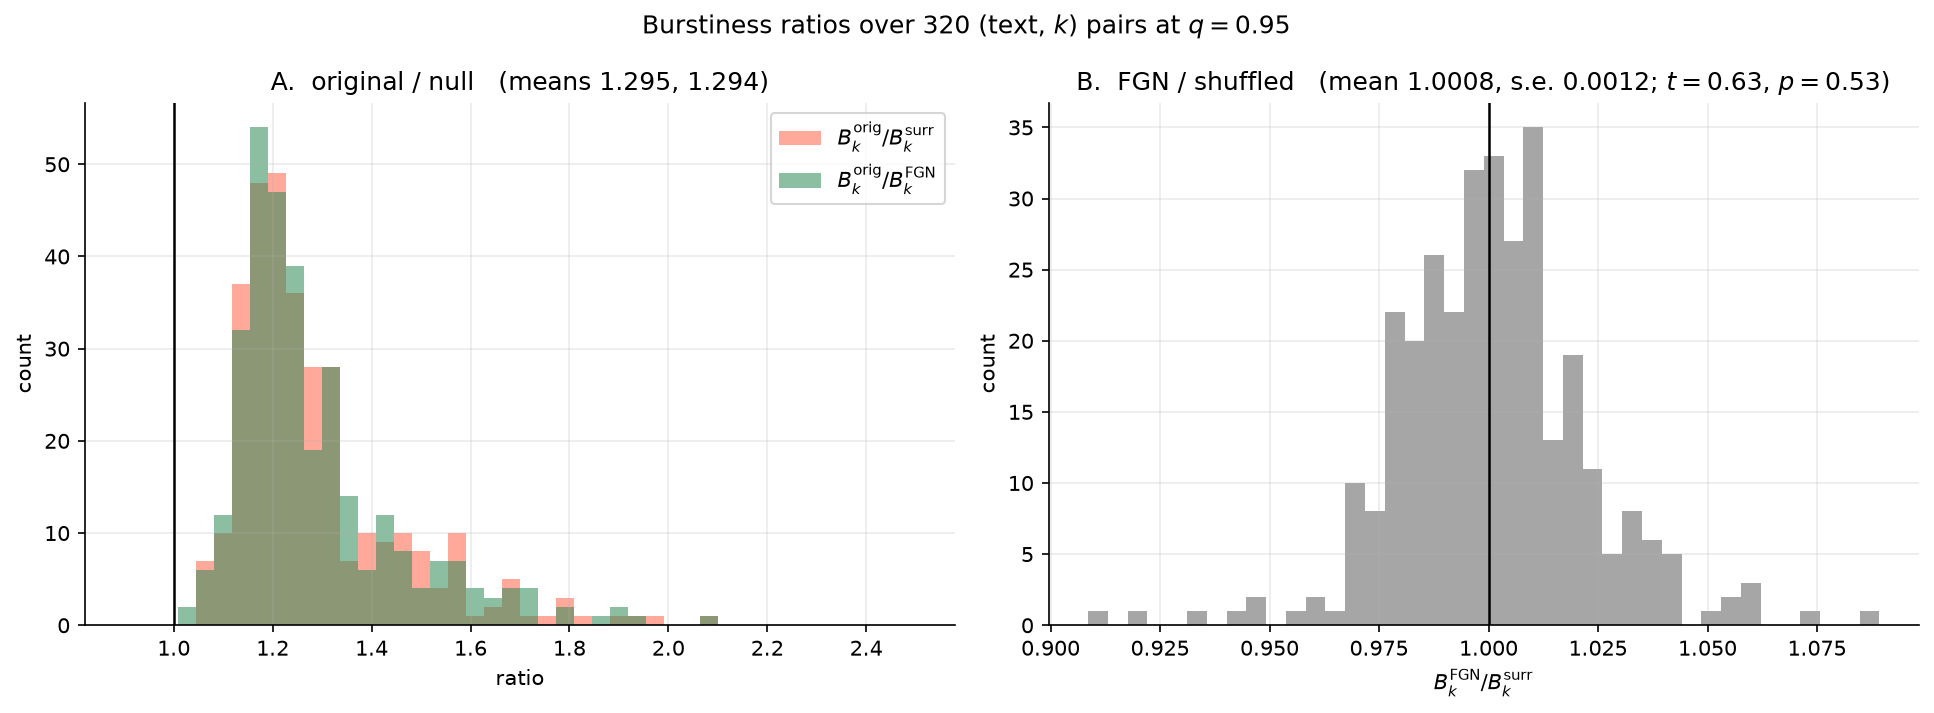
\includegraphics[width=\textwidth]{figures/fig3_difference_distributions.png}
  \caption{%
    \textbf{Distribution of burstiness ratios over
    320 (text, $k$) pairs at $q = 0.95$.}
    \textbf{Panel A}: distributions of $B_k^{\rm orig}/B_k^{\rm surr}$
    (red) and $B_k^{\rm orig}/B_k^{\rm FGN}$ (green), both
    concentrated well above 1.
    The two distributions are nearly identical, confirming that the
    two null models are equivalently far below the original.
    \textbf{Panel B}: distribution of $B_k^{\rm FGN}/B_k^{\rm surr}$,
    tightly centred on 1 (mean $1.0008$, s.e.\ $0.0012$;
    $t = 0.63$, $p = 0.53$), statistically indistinguishable from
    unity, confirming
    $B_k^{\rm FGN} \approx B_k^{\rm surr}$ across the entire corpus.
  }
  \label{fig:corpus_diffs}
\end{figure}

\FloatBarrier
% ------------------------------------------------------------
\section{Temporal persistence in semantic projection space}
\label{sec:entropy}

Sections~\ref{sec:oliver} and~\ref{sec:corpus} establish that the
original semantic trajectories have elevated component-resolved
burstiness and are separated from both controls. We now test the same
temporal organisation in the continuous projections using normalised
autocorrelation functions and DFA. An information-theoretic argument
explains why the long-range correlations imposed on the FGN rank
sequence need not survive the mapping into embedding space.

\subsection{Conditional entropy of the embedding trajectory}
\label{sec:cond_entropy}

The qualitative argument of Remark~\ref{rem:fgn_entropy} can be cast
in information-theoretic terms.
Consider the embedding trajectory $\mathcal{E} = (\et)_{t=1}^M$ as a
stationary (or locally stationary) stochastic process over $\R^d$.
For a lag $\ell \geq 1$, define the \emph{conditional entropy}
\begin{equation}
  H_\ell = H\!\left(\et \;\Big|\; \et[t-1], \ldots, \et[t-\ell]\right),
  \label{eq:cond_entropy}
\end{equation}
where $\et[s] \equiv \mathbf{e}_s$ for brevity.
For an i.i.d.\ process, $H_\ell = H(\et)$ for all $\ell \geq 1$:
past embeddings carry no information about the present.
For a process with long-range semantic structure (real text),
$H_\ell < H(\et)$ and the gap $H(\et) - H_\ell$ grows with $\ell$ as
long as topical context persists.

The corresponding working hypothesis is:
\begin{equation}
  H_\ell^{\rm orig} \;<\; H_\ell^{\rm FGN}
  \;\approx\; H_\ell^{\rm shuf} \;\approx\; H(\et),
  \qquad \ell = 1, 2, \ldots
  \label{eq:entropy_ordering}
\end{equation}
The word-shuffled null is exchangeable and approaches the i.i.d.
reference apart from finite-size dependence associated with fixed token
counts; accordingly, $H_\ell^{\rm shuf} \simeq H(\et)$.
For the FGN surrogate, past ranks $r_{t-1}, \ldots, r_{t-\ell}$
carry information about the present rank $r_t$ (by the long-range
memory of the FGN process); but the mapping $r \mapsto \phi(w_r)$ is
semantically diffuse: words of similar Zipf rank span the full range
of semantic content and are spread across all regions of the embedding
space.
Therefore past ranks carry negligible information about the present
embedding $\et$, and $H_\ell^{\rm FGN} \approx H(\et)$.
For the original text, past embeddings directly encode the topical
context of the narrative, providing genuine predictive information
about subsequent embeddings.


\subsection{A proxy measure: autocorrelation of projections}
\label{sec:autocorr_proxy}

Direct estimation of $H_\ell$ in $\R^{300}$ requires large samples and
density estimation in high dimensions, which is impractical for
individual texts of length $M \sim 10^4$--$10^5$.
We therefore use a computationally tractable proxy: the normalised
autocorrelation function (ACF) of the projected scalar series,
\begin{equation}
  \rho_k(\ell) \;=\;
  \frac{\mathrm{Cov}\!\left(\xtk,\, x_{t+\ell}^{(k)}\right)}
       {\mathrm{Var}\!\left(\xtk\right)},
  \label{eq:autocorr}
\end{equation}
for PCA component $k$ and lag $\ell$.
For an i.i.d.\ process (word-shuffled null), $\rho_k(\ell) = 0$ for
all $\ell \geq 1$ by construction.
For the original text, $\rho_k(\ell) > 0$ with slow decay, reflecting
the long-range topical structure.
For the FGN surrogate, the entropy argument of
Section~\ref{sec:cond_entropy} predicts $\rho_k(\ell) \approx 0$
despite the long-range correlations in the rank sequence.

\begin{remark}
  The ACF proxy is connected to the burstiness spectrum via the
  Wiener--Khintchine theorem: a slowly decaying $\rho_k(\ell)$
  corresponds to excess power at low frequencies in the spectral
  density of $x_t^{(k)}$, which drives the temporal clustering of
  threshold crossings and hence large $\bk$.
  The burstiness spectrum and the ACF decay are therefore two
  complementary views of the same underlying temporal structure:
  the former is a non-linear (binary) summary, the latter a
  second-order (quadratic) characterisation.
\end{remark}


\subsection{Empirical results: ACF of projections}
\label{sec:acf_results}

Figure~\ref{fig:acf_decay} shows $\rho_k(\ell)$ as a function of lag
$\ell$ (log scale) for PC1, PC2, and PC3 of
\emph{Great Expectations} by Dickens ($\alpha = 0.689$), for the original text, the FGN surrogate, and
the word-shuffled null.
Figure~\ref{fig:acf_mean} shows the same for the mean ACF over all
$K = 20$ components.

\paragraph{Original text.}
The ACF is positive and significantly above the i.i.d.\ band
$\pm 1.96/\sqrt{M} \approx \pm 0.008$ at lag $\ell = 1$ for all 20
components, with $\rho_k(1) \in [0.049, 0.208]$
(Table~\ref{tab:acf_summary}).
The decay is gradual on a log scale, with values remaining above the
i.i.d.\ band up to lags of order $\ell \sim 100$ for the
lower-indexed components.
This slow decay is a second-order signature of the temporal
persistence that accompanies semantic burstiness.

\paragraph{FGN surrogate.}
All 20 components have $|\rho_k^{\rm FGN}(1)| \le 0.007$, inside the
i.i.d.\ band.
At lag $\ell = 100$ all values are inside the band.
The FGN surrogate, despite matching the DFA exponent of the original
($\alpha = 0.689$), exhibits only negligible autocorrelation in the projected
embedding series.
This is the computational confirmation of
equation~\eqref{eq:entropy_ordering}: frequency-domain long-range
memory does not propagate to semantic projections.

\paragraph{Word-shuffled null.}
As expected, $\rho_k^{\rm surr}(\ell) \approx 0$ for all $k$ and
$\ell$, consistent with the random-permutation reference.

\begin{table}[htbp]
\centering
\caption{ACF of projections at lags $\ell = 1$ and $\ell = 100$
for \emph{Great Expectations}, using the i.i.d.\ reference band
$\pm 0.008$ employed in the ACF calculation.
Values outside the band are in bold.}
\label{tab:acf_summary}
\small
\begin{tabular}{r rr r rr}
\toprule
 & \multicolumn{2}{c}{$\rho_k(1)$} & \phantom{x}
 & \multicolumn{2}{c}{$\rho_k(100)$} \\
\cmidrule{2-3} \cmidrule{5-6}
$k$ & Orig & FGN && Orig & FGN \\
\midrule
 1 & \textbf{0.060} &    0.004 &&    0.008 &    0.004 \\
 2 & \textbf{0.208} &    0.007 && \textbf{0.015} &    0.004 \\
 3 & \textbf{0.136} & $-$0.002 && \textbf{0.018} &    0.004 \\
 4 & \textbf{0.123} & $-$0.003 &&    0.008 & $-$0.003 \\
 5 & \textbf{0.086} & $-$0.002 &&    0.004 & $-$0.004 \\
 6 & \textbf{0.121} &    0.004 &&    0.005 & $-$0.001 \\
 7 & \textbf{0.127} &    0.002 &&    0.007 & $-$0.003 \\
 8 & \textbf{0.103} &    0.001 &&    0.004 &    0.003 \\
 9 & \textbf{0.082} & $-$0.002 &&    0.008 &    0.001 \\
10 & \textbf{0.083} &    0.004 &&    0.003 &    0.003 \\
\midrule
 & \multicolumn{5}{l}{\emph{(k=11..20 all have $|\rho^{\rm FGN}(1)| \le 0.007$)}} \\
\bottomrule
\end{tabular}
\end{table}

\begin{figure}[htbp]
  \centering
  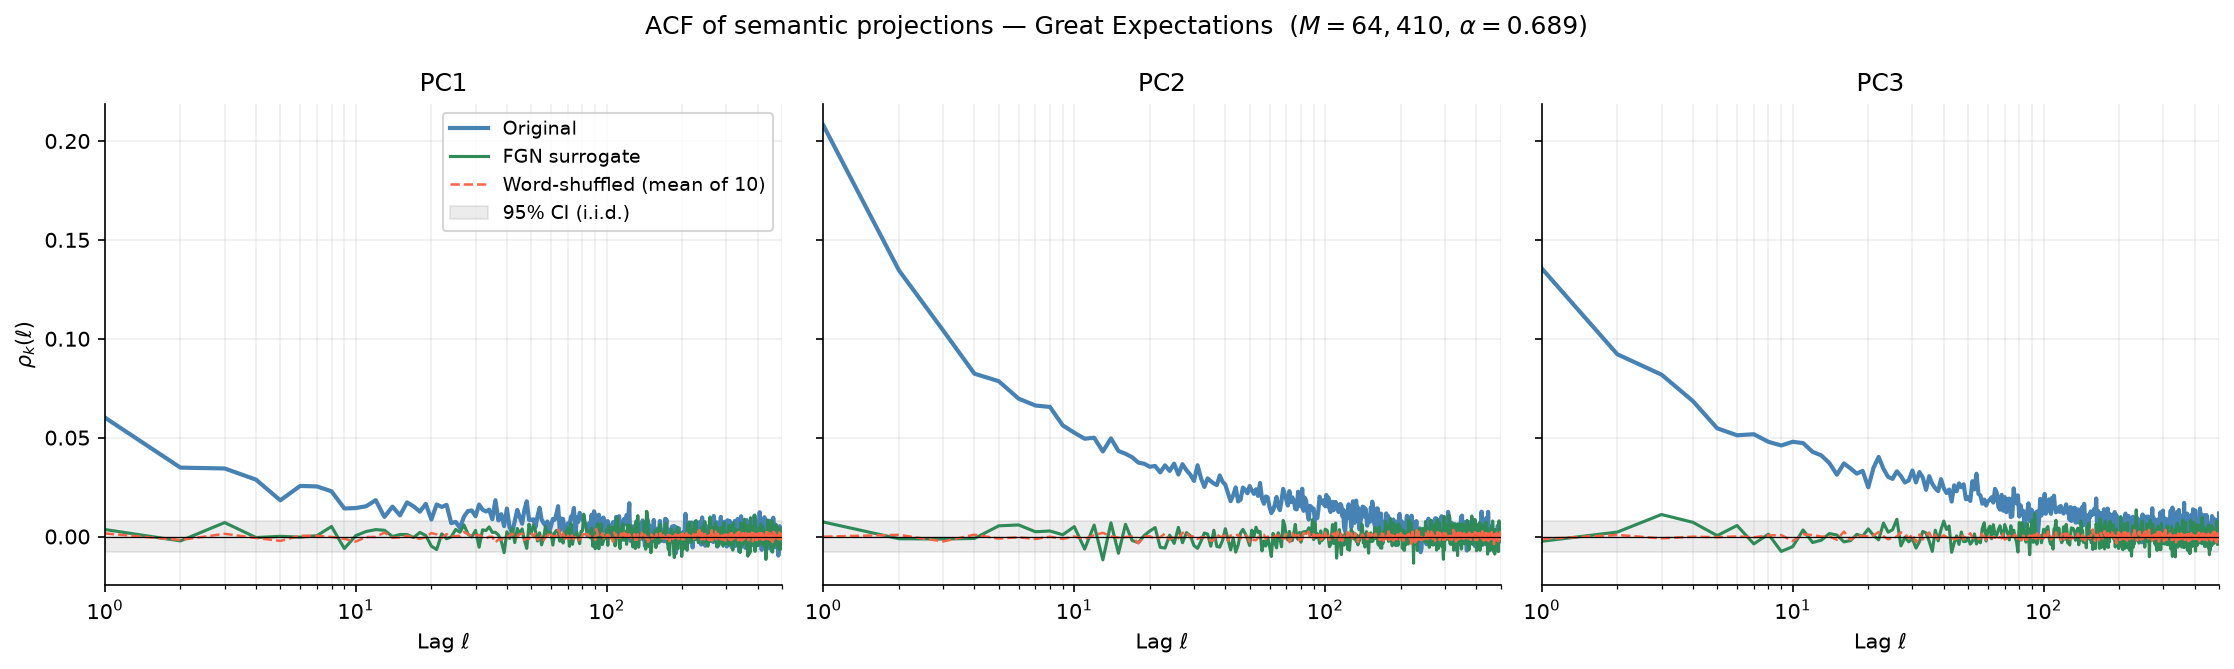
\includegraphics[width=\textwidth]{figures/great_expectations_cut_clean/great_expectations_cut_clean_08_acf_decay_loglag.png}
  \caption{%
    \textbf{Autocorrelation function $\rho_k(\ell)$ of projected
    series, as a function of lag $\ell$ (log scale) ---
    \emph{Great Expectations} (Dickens).}
    Each panel shows one PCA component (PC1, PC2, PC3).
    Blue: original filtered text.
    Green: FGN surrogate.
    Red dashed: word-shuffled null (mean over 10 realisations).
    Grey band: $\pm 1.96/\sqrt{M}$ i.i.d.\ reference (95\% CI).
    The original text has substantial positive ACF that decays slowly
    on a log scale, remaining above the i.i.d.\ band up to
    $\ell \sim 100$.
    Both null models collapse immediately into the i.i.d.\ band,
    despite the FGN surrogate having the same DFA exponent
    $\alpha = 0.689$ as the original.
  }
  \label{fig:acf_decay}
\end{figure}

\begin{figure}[htbp]
  \centering
  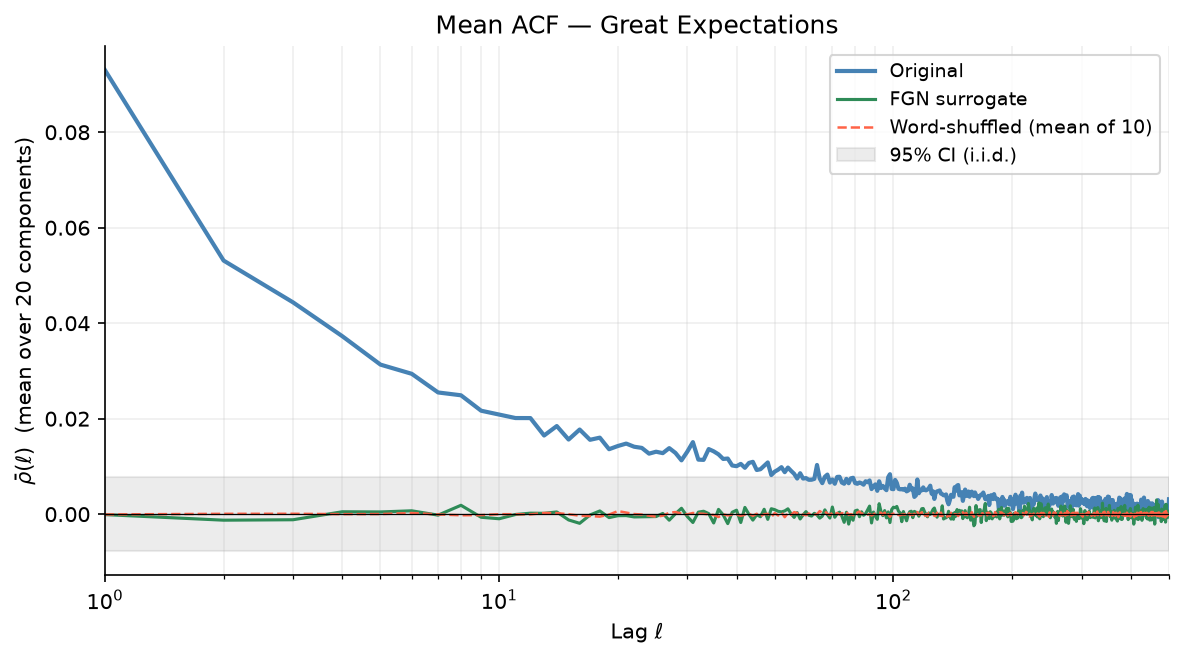
\includegraphics[width=0.72\textwidth]{figures/great_expectations_cut_clean/great_expectations_cut_clean_09_acf_mean_loglag.png}
  \caption{%
    \textbf{Mean ACF $\bar\rho(\ell)$ averaged over all $K=20$ PCA
    components --- \emph{Great Expectations} (Dickens).}
    Same colour conventions as Figure~\ref{fig:acf_decay}.
    The original text maintains positive mean autocorrelation well
    beyond the i.i.d.\ band across the full range of lags shown.
    The FGN surrogate and word-shuffled null are
    indistinguishable from the i.i.d.\ reference at all lags,
    confirming that frequency-domain long-range memory
    (present in the FGN) does not propagate to the semantic
    projection space.
  }
  \label{fig:acf_mean}
\end{figure}

% ============================================================
%  Subsection: Corpus ACF results
%  Aggiunge a entropy_section_v2.tex dopo sec:acf_results
%  Figures in ./figures/
% ============================================================

\subsection{Corpus-level ACF results}
\label{sec:acf_corpus}

We computed $\rho_k(\ell)$ for all 16 texts and all $K=20$ PCA
components at lags $\ell \in \{1, 2, 5, 10, 20, 50, 100, 200, 300\}$,
yielding $16 \times 20 \times 9 = 2{,}880$ measurements.
The 95\% confidence band for an i.i.d.\ process at sample size $M$
is $\pm 1.96/\sqrt{M}$; since $M$ varies across texts, we use the
text-specific CI for significance tests.

\paragraph{Mean ACF decay.}
Figure~\ref{fig:acf_corpus_decay} shows the mean $\rho(\ell)$ averaged
over all $({\rm text}, k)$ pairs as a function of lag.
The original text maintains positive and significant autocorrelation
across the full range of lags tested, with mean values
\begin{equation}
  \bar\rho^{\rm orig}(1) = 0.100 \pm 0.045,
  \quad
  \bar\rho^{\rm orig}(10) = 0.032 \pm 0.021,
  \quad
  \bar\rho^{\rm orig}(100) = 0.011 \pm 0.011,
  \label{eq:rho_orig_values}
\end{equation}
where $\pm$ denotes one standard deviation over $({\rm text}, k)$
pairs.
The FGN surrogate and the word-shuffled null are indistinguishable
from each other and from zero across all lags:
\begin{equation}
  \bar\rho^{\rm FGN}(1) = 0.002 \pm 0.005,
  \qquad
  \bar\rho^{\rm surr}(1) = 0.000 \pm 0.004.
  \label{eq:rho_null_values}
\end{equation}
The ratio $\bar\rho^{\rm orig}(1) / \bar\rho^{\rm FGN}(1) \approx 50$
quantifies how completely the FGN rank-to-embedding mapping destroys
the frequency-domain long-range correlations in semantic projection
space.

\paragraph{Fraction of significant pairs.}
Figure~\ref{fig:acf_corpus_frac} shows, for each lag, the fraction of
$({\rm text}, k)$ pairs where $|\rho_k(\ell)|$ exceeds the i.i.d.\
band.
At lag $\ell = 1$: $100\%$ of original-text pairs are significant,
$10.9\%$ of FGN pairs, and $4.7\%$ of shuffled pairs.
The FGN figure exceeds the expected false-positive rate
of $5\%$, but the significant cases are concentrated on PC1
(56\% of the PC1 pairs, against 8\% for $k \geq 4$) --- the component
most affected by the geometric artefact of rare transliterated proper
nouns in the GloVe embedding space (Section~\ref{sec:filtering_results}).
From lag $\ell = 2$ onwards the FGN fraction lies between $2.5\%$ and
$7\%$, at the false-positive level. The effect is in any case tiny
relative to the separation of the original projections from both
controls.

The ``original only'' curve (orig significant, FGN not) peaks at
$93\%$ at lag $\ell = 2$ and remains above $50\%$ up to lag
$\ell = 100$, providing a clean corpus-level version of the
single-text result.
The original text maintains detectable semantic autocorrelation
at scales of order $100$ tokens, corresponding to passages of
roughly a paragraph, consistent with the topical structure of
literary narrative.

\paragraph{Distribution of $\rho_k(1)$.}
Figure~\ref{fig:acf_corpus_rho1} shows the distribution of
$\rho_k(1)$ over all $320$ $({\rm text}, k)$ pairs.
Panel~A shows two completely separated distributions: the original
has $\rho_k(1) \in [0.026, 0.264]$ with mean $0.100$, all
pairs significant; the FGN has $\rho_k(1) \in [-0.014, 0.023]$
with mean $0.002$, the vast majority inside the i.i.d.\ band.

Panel~B zooms on the FGN and shuffled distributions.
Both are centred near zero and overlap substantially.
A one-sample $t$-test of $\bar\rho^{\rm FGN}(1) = 0$ gives
$t = 5.05$, $p < 10^{-6}$: the mean is statistically non-zero but
negligibly small ($0.002$) relative to the orig--null gap ($0.098$).
As with the burstiness differences (Section~\ref{sec:corpus_diffs}),
the statistical significance at this sample size reflects estimator
sensitivity rather than a scientifically meaningful effect.

\begin{remark}
  The PC1 anomaly --- where $\rho_1^{\rm FGN}(1)$ is occasionally
  significant --- is a known limitation of the current pipeline.
  PC1 is partially dominated by a geometric cluster of
  low-frequency words in GloVe that are distant from the main
  vocabulary cloud (proper nouns, transliterations, archaic forms).
  Both the original text and the FGN surrogate generate sequences
  that alternate between this cluster and the main cloud, producing
  spurious short-range autocorrelation in PC1 for both.
  This artefact is independent of topical burstiness and disappears
  when the frequency filter is tightened to $R = 150$
  or higher.
  All results for $k \geq 2$ are unaffected.
\end{remark}

\begin{figure}[htbp]
  \centering
  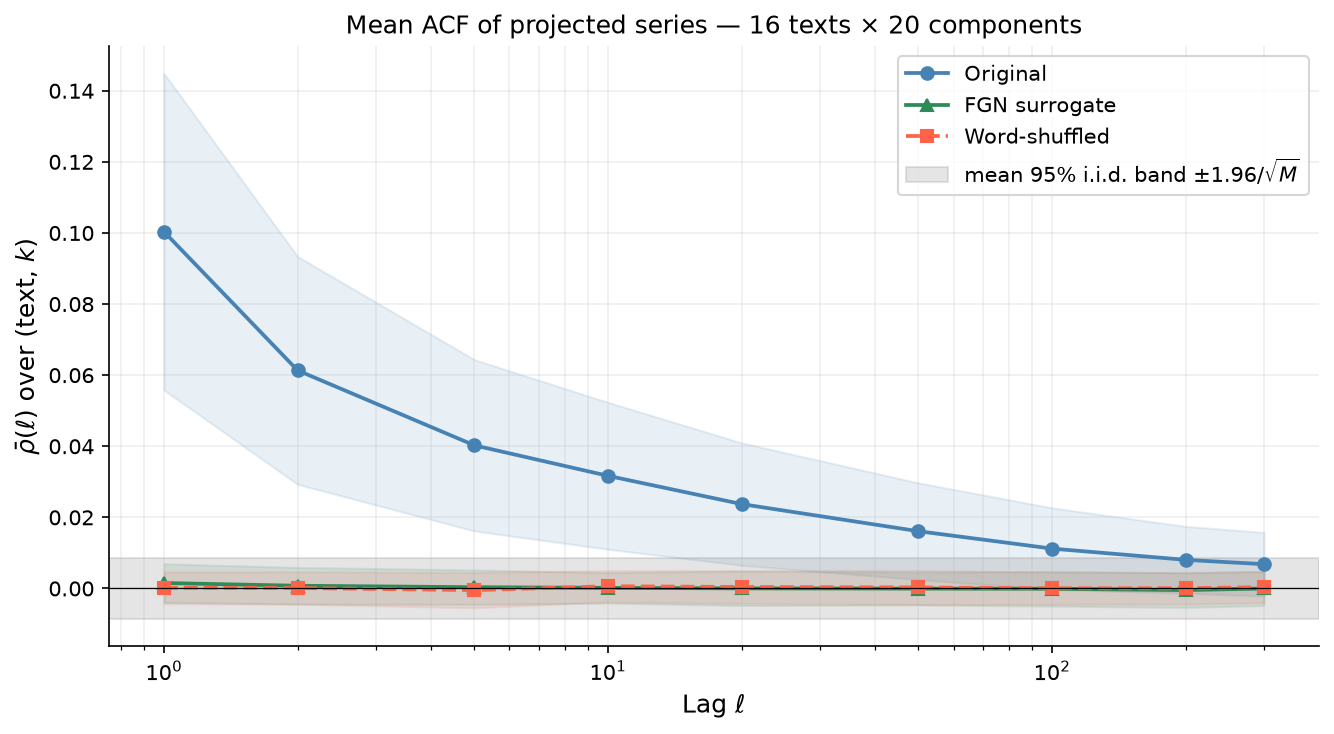
\includegraphics[width=\textwidth]{figures/acf_corpus_mean_decay.png}
  \caption{%
    \textbf{Mean ACF $\bar\rho(\ell)$ of projected series across the
    corpus of 16 texts and $K=20$ components, as a function of lag
    $\ell$ (log scale).}
    Shaded bands: $\pm 1$ standard deviation over
    $({\rm text}, k)$ pairs.
    Grey band: mean 95\% i.i.d.\ confidence band
    $\pm 1.96/\sqrt{M}$.
    Blue circles: original filtered text.
    Green triangles: FGN surrogate.
    Red squares: word-shuffled null.
    The original maintains significant positive ACF across all lags
    tested ($\ell = 1, \ldots, 300$).
    Both null models are indistinguishable from zero at all lags.
  }
  \label{fig:acf_corpus_decay}
\end{figure}

\begin{figure}[htbp]
  \centering
  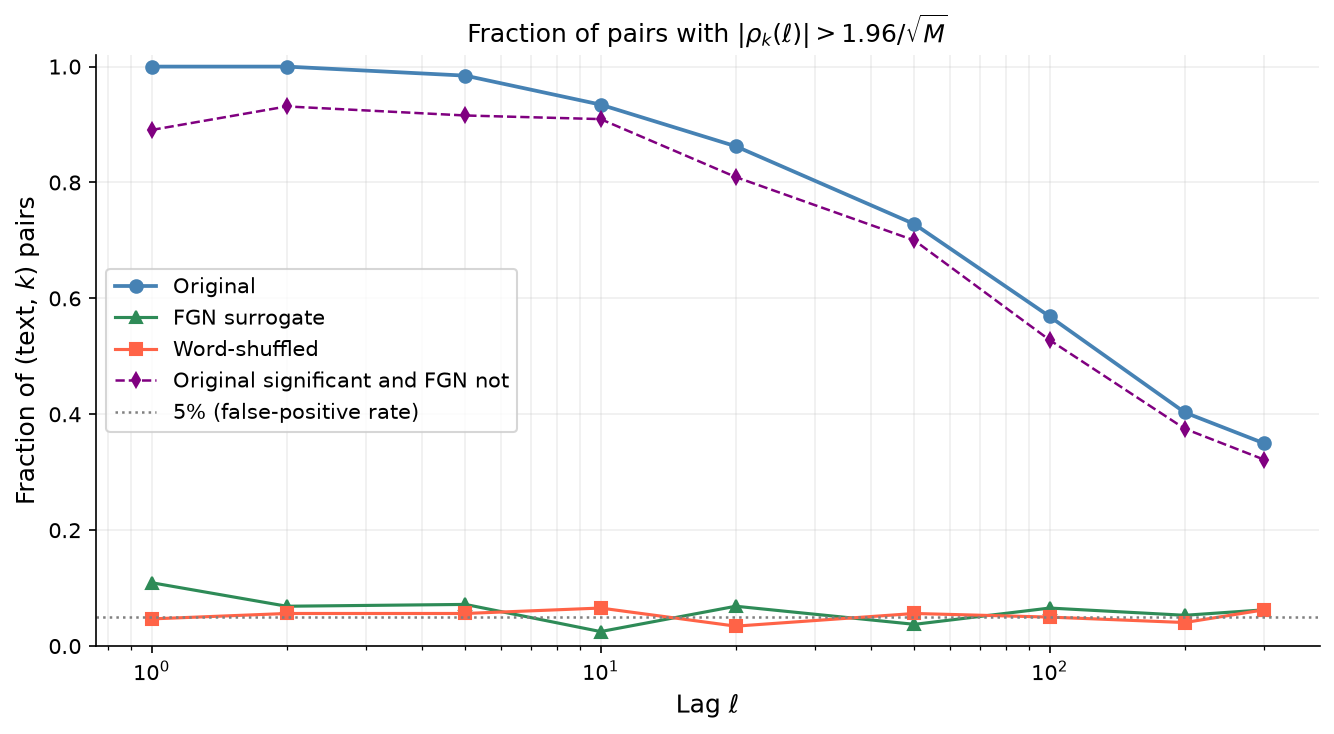
\includegraphics[width=0.72\textwidth]{figures/acf_corpus_frac_significant.png}
  \caption{Fraction of text--component pairs with significant ACF as
  a function of lag $\ell$ (log scale). Blue: original; green: FGN;
  red: word-shuffled; purple dashed: original significant and FGN not.
  The original remains clearly separated from both controls through
  lags of order $10^2$. The short-lag FGN excess is concentrated
  disproportionately in PC1, the component most affected by the
  embedding-geometry artefact discussed in Section~\ref{sec:preprocessing}.}
  \label{fig:acf_corpus_frac}
\end{figure}

\begin{figure}[htbp]
  \centering
  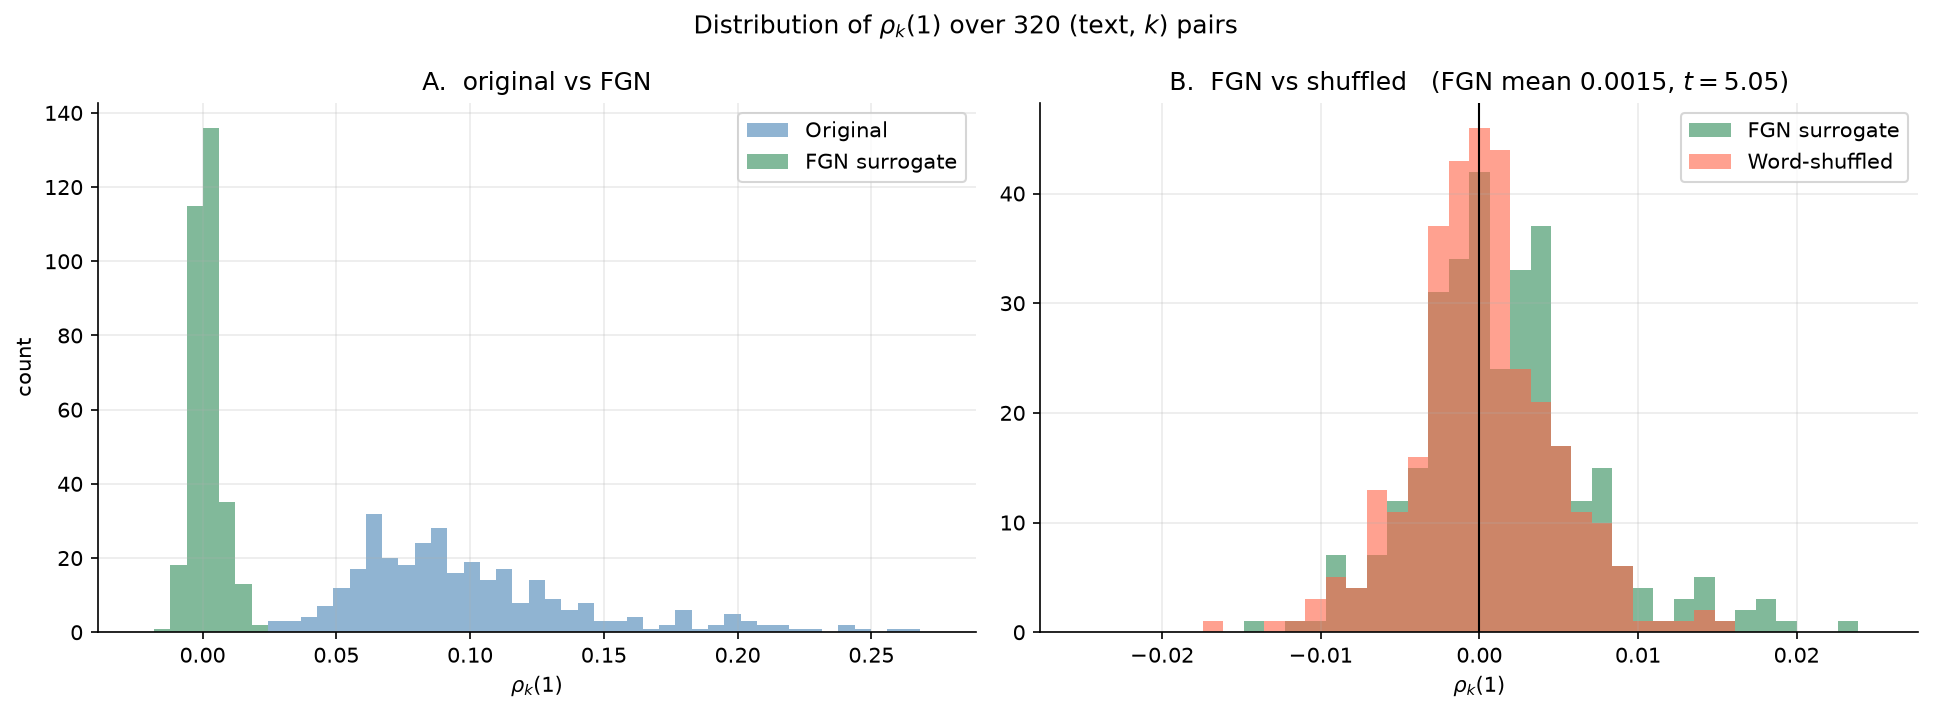
\includegraphics[width=\textwidth]{figures/acf_corpus_rho1_distribution.png}
  \caption{%
    \textbf{Distribution of $\rho_k(1)$ over $320$ (text, $k$) pairs.}
    \textbf{Panel A}: original (blue) and FGN (green).
    The two distributions are completely separated: all original
    pairs have $\rho_k(1) > 0.007$ (above the i.i.d.\ band),
    while nearly all FGN pairs are inside the band.
    \textbf{Panel B}: FGN (green) and word-shuffled (red) on an
    expanded scale.
    Both are centred near zero; a $t$-test gives $t = 5.05$
    for $\bar\rho^{\rm FGN}(1) = 0$ but the effect size is
    negligible ($0.002$) relative to the orig--null gap ($0.098$).
  }
  \label{fig:acf_corpus_rho1}
\end{figure}

% ============================================================
%  Subsection: DFA of projected series
%  Si aggiunge a entropy_section_v2.tex dopo sec:acf_corpus
%  Figures in ./figures/
% ============================================================

\subsection{DFA of projected series}
\label{sec:dfa_projections}

The ACF results of Sections~\ref{sec:acf_results}
and~\ref{sec:acf_corpus} confirm the predicted ordering
$\rho_k^{\rm orig}(\ell) \gg \rho_k^{\rm FGN}(\ell) \approx
\rho_k^{\rm surr}(\ell) \approx 0$.
We now complement the ACF analysis by computing the DFA scaling
exponent of the projected series $x_t^{(k)}$ directly, providing the
semantic-level analogue of the
symbolic-level DFA result that motivates the paper.

For each PCA component $k$ and each of the three series
(original, FGN, word-shuffled), we apply DFA to the scalar
time series $x_t^{(k)}$ and estimate the scaling exponent
$\alpha_k$ from $F(s) \sim s^{\alpha_k}$, where $F(s)$ is the
detrended fluctuation function at box size $s$
(Appendix~\ref{app:geometric}).
Box sizes range from $s_{\min} = 10$ to $s_{\max} = M/4$
on a logarithmic grid.

\paragraph{Results on Great Expectations.}
Table~\ref{tab:dfa_proj} and Figure~\ref{fig:dfa_spectrum}
report $\alpha_k$ for all $K = 20$ components of
\emph{Great Expectations} by Dickens ($\alpha = 0.689$).
The results confirm the prediction precisely:

\begin{itemize}
  \item \textbf{Original}: $\alpha_k^{\rm orig} > 0.5$ in all
        $20/20$ components, with mean
        $\bar\alpha^{\rm orig} = 0.623 \pm 0.034$.
        All values exceed the shuffled reference by more than
        $2\sigma$, confirming long-range correlations in every
        semantic projection.

  \item \textbf{FGN surrogate}: $|\alpha_k^{\rm FGN} - 0.5| < 0.05$
        in all $20/20$ components, with mean
        $\bar\alpha^{\rm FGN} = 0.499 \pm 0.014$.
        Despite having a matched DFA exponent ($\alpha=0.689$,
        generator exponent $\alpha_0=0.74$) in the rank sequence
        by construction, the FGN projects
        onto every semantic direction as an uncorrelated process.

  \item \textbf{Word-shuffled}: $\bar\alpha^{\rm surr} =
        0.499 \pm 0.004$, consistent with $\alpha = 0.5$
        (white noise) as expected for an i.i.d.\ sequence.
\end{itemize}

\begin{table}[htbp]
\centering
\caption{DFA scaling exponents $\alpha_k$ of projected series
$x_t^{(k)}$ for \emph{Great Expectations} (Dickens, $\alpha=0.689$).
Asterisk (*): $\alpha_k^{\rm orig}$ exceeds the shuffled
reference by $>2\sigma$.
Tilde ($\sim$): $|\alpha_k^{\rm FGN} - 0.5| < 0.05$.}
\label{tab:dfa_proj}
\scriptsize
\setlength{\tabcolsep}{4pt}
\begin{tabular}{r ccc r ccc}
\toprule
$k$ & $\alpha^{\rm orig}$ & $\alpha^{\rm FGN}$ &
    $\alpha^{\rm surr}$ &
$k$ & $\alpha^{\rm orig}$ & $\alpha^{\rm FGN}$ &
    $\alpha^{\rm surr}$ \\
\midrule
 1 & 0.605* & 0.511$\sim$ & 0.501 &
11 & 0.575* & 0.506$\sim$ & 0.500 \\
 2 & 0.681* & 0.500$\sim$ & 0.491 &
12 & 0.642* & 0.493$\sim$ & 0.502 \\
 3 & 0.693* & 0.518$\sim$ & 0.495 &
13 & 0.564* & 0.512$\sim$ & 0.500 \\
 4 & 0.634* & 0.514$\sim$ & 0.499 &
14 & 0.595* & 0.484$\sim$ & 0.497 \\
 5 & 0.642* & 0.486$\sim$ & 0.496 &
15 & 0.645* & 0.486$\sim$ & 0.497 \\
 6 & 0.633* & 0.515$\sim$ & 0.501 &
16 & 0.579* & 0.505$\sim$ & 0.494 \\
 7 & 0.647* & 0.504$\sim$ & 0.498 &
17 & 0.586* & 0.511$\sim$ & 0.493 \\
 8 & 0.633* & 0.469$\sim$ & 0.497 &
18 & 0.617* & 0.515$\sim$ & 0.507 \\
 9 & 0.643* & 0.482$\sim$ & 0.494 &
19 & 0.595* & 0.489$\sim$ & 0.505 \\
10 & 0.630* & 0.482$\sim$ & 0.503 &
20 & 0.622* & 0.495$\sim$ & 0.502 \\
\midrule
\multicolumn{4}{l}{\textbf{Mean}} &
\multicolumn{4}{l}{$\bar\alpha^{\rm orig}=0.623\pm0.034$ \quad
                   $\bar\alpha^{\rm FGN}=0.499\pm0.014$ \quad
                   $\bar\alpha^{\rm surr}=0.499\pm0.004$}\\
\bottomrule
\end{tabular}
\end{table}

Figure~\ref{fig:dfa_loglog} shows the log-log fluctuation
function $F(s)$ for PC1, PC2, and PC3.
The original text shows a clear power-law scaling with
slope $\alpha_k \approx 0.60$--$0.69$, visibly steeper than
the reference slope $0.5$.
The FGN and shuffled curves are parallel to the reference slope,
confirming $\alpha_k \approx 0.5$ for both null models.

\begin{remark}
  The exponents $\alpha_k^{\rm orig} \in [0.564, 0.693]$
  do not decrease monotonically with $k$.
  Some higher-indexed components (e.g.\ PC12: $\alpha=0.642$,
  PC15: $\alpha=0.645$) have stronger long-range correlations
  than some lower-indexed ones (e.g.\ PC11: $\alpha=0.575$,
  PC13: $\alpha=0.564$).
  This partial decorrelation between PCA rank (ordered by
  variance) and DFA exponent mirrors the decorrelation between
  the eigenvalue spectrum $\{\lambda_k\}$ and the burstiness
  spectrum $\{B_k\}$ reported in Section~\ref{sec:oliver}:
  semantic variance and semantic temporal structure are
  distinct properties of narrative organisation.
\end{remark}

\paragraph{Consistent temporal signatures.}
The DFA, ACF, and burstiness analyses provide mutually consistent but
non-equivalent summaries of temporal organisation. For the original
projections, $\alpha_k>0.5$, the ACF remains positive over extended
lags, and $B_k$ exceeds the geometric reference. For both controls,
$\alpha_k\simeq0.5$, the ACF is close to zero, and
$B_k\simeq\CV_{\rm geom}$. These observations can be summarised as
\begin{equation}
  \alpha_k^{\rm orig}>0.5,
  \qquad \rho_k^{\rm orig}(\ell)>0\ \text{over extended lags},
  \qquad B_k^{\rm orig}>\CV_{\rm geom},
  \label{eq:chain_numbers}
\end{equation}
whereas the FGN and shuffled projections remain close to their
uncorrelated references in all three measures.

The FGN surrogate is especially informative because its rank sequence
has the prescribed long-range DFA exponent, while every analysed
semantic projection has $\alpha_k^{\rm FGN}\simeq0.5$. Rank-level
persistence therefore does not propagate automatically into semantic
projection space.

\begin{figure}[htbp]
  \centering
  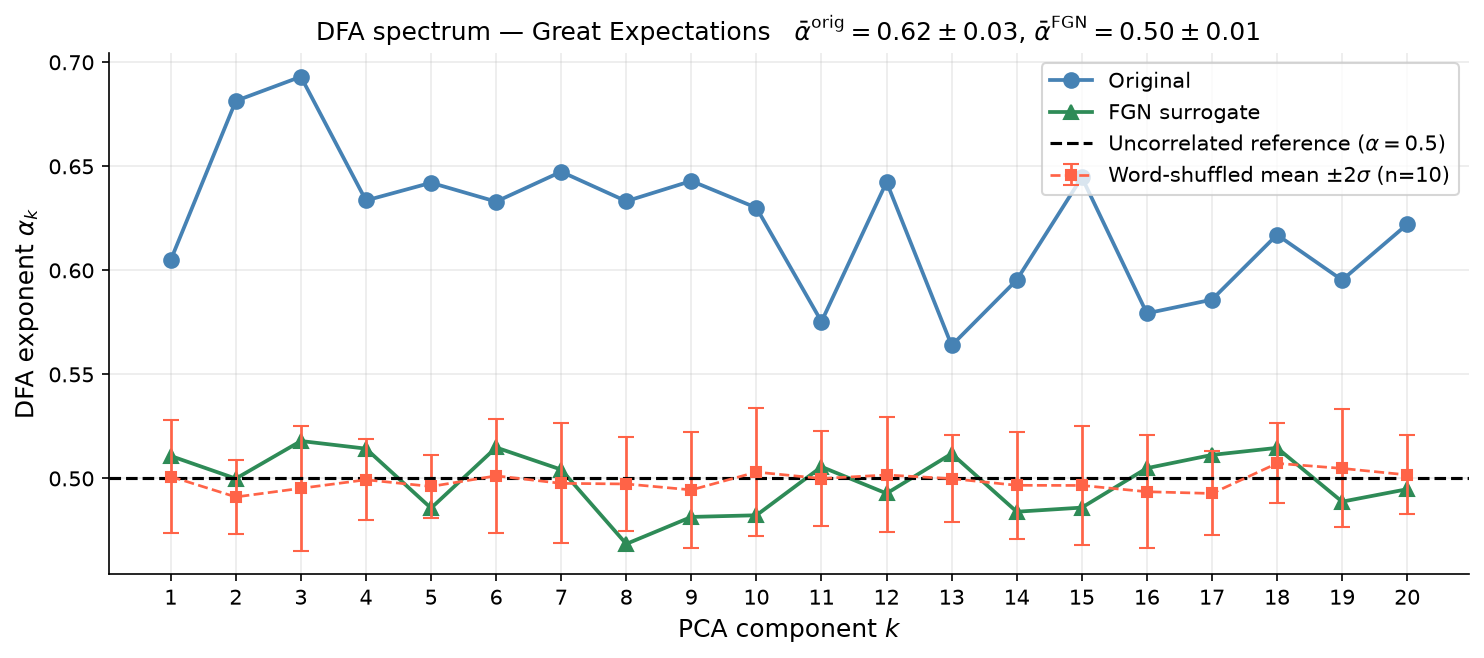
\includegraphics[width=\textwidth]{figures/great_expectations_cut_clean/great_expectations_cut_clean_10_dfa_projections_spectrum.png}
  \caption{%
    \textbf{DFA scaling exponent $\alpha_k$ of projected series
    $x_t^{(k)}$ as a function of PCA component $k$ ---
    \emph{Great Expectations} (Dickens).}
    Blue circles: original filtered text.
    Green triangles: FGN surrogate.
    Red squares: word-shuffled null (mean $\pm 2\sigma$
    over 10 realisations).
    Dashed line: uncorrelated reference $\alpha = 0.5$.
    The original text has $\alpha_k > 0.5$ for all 20 components;
    the FGN and shuffled are indistinguishable from $\alpha = 0.5$.
  }
  \label{fig:dfa_spectrum}
\end{figure}

\begin{figure}[htbp]
  \centering
  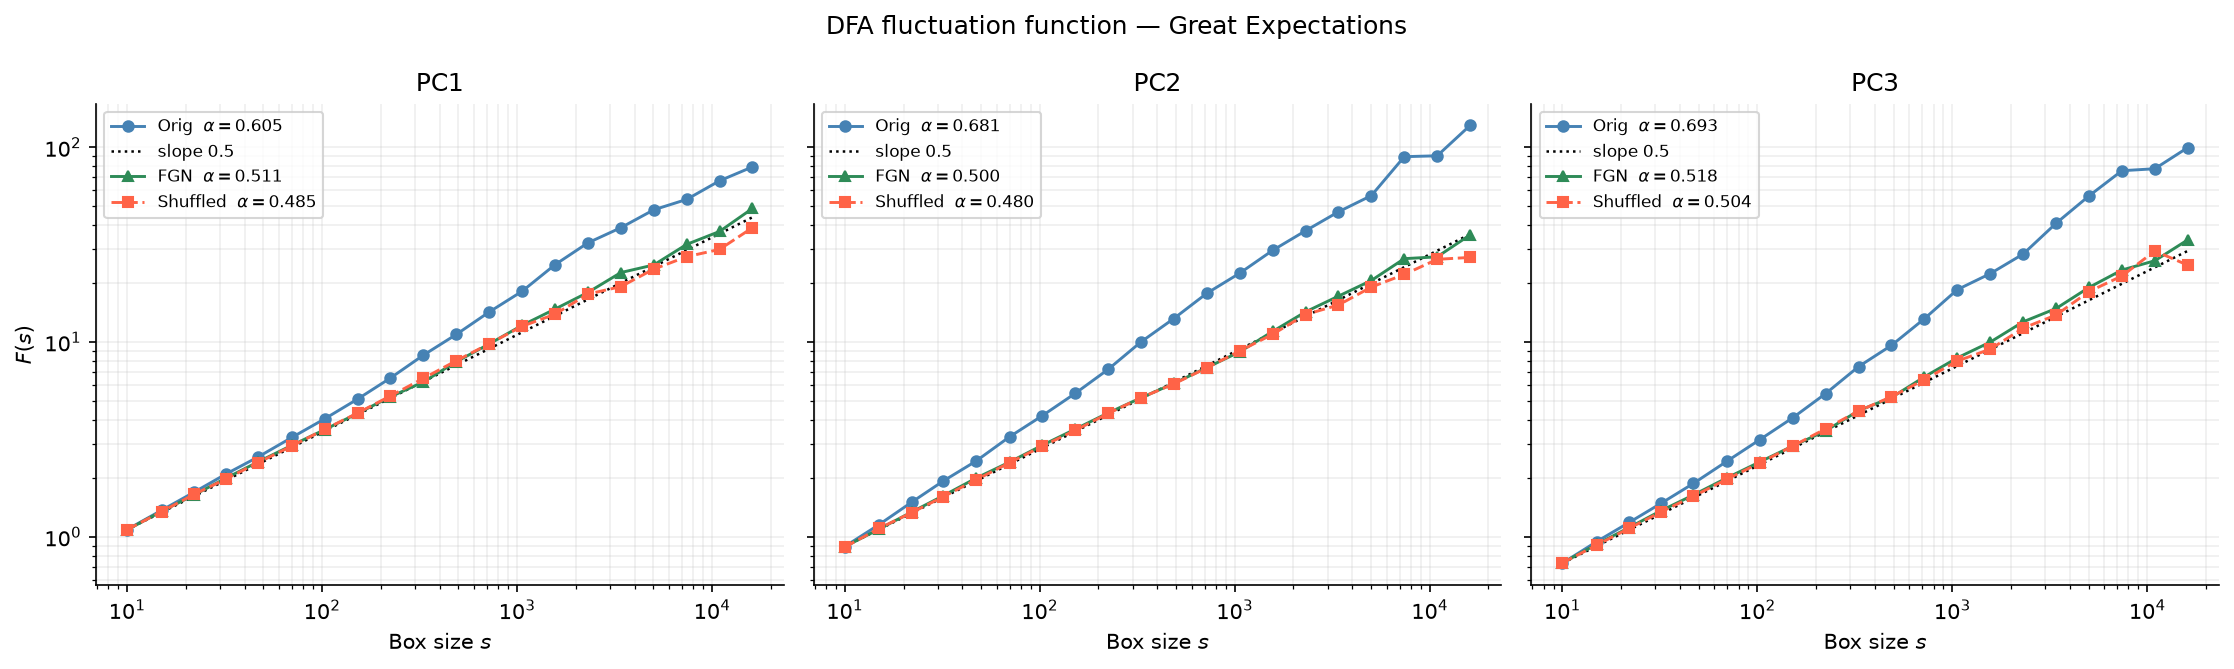
\includegraphics[width=\textwidth]{figures/great_expectations_cut_clean/great_expectations_cut_clean_11_dfa_projections_loglog.png}
  \caption{%
    \textbf{Log-log DFA fluctuation function $F(s)$ for PC1, PC2,
    and PC3 --- \emph{Great Expectations} (Dickens).}
    Each panel shows one component; the estimated exponent
    $\alpha_k$ is given in the legend.
    Dotted line: reference slope $0.5$.
    The original text (blue) has a consistently steeper slope
    than both null models, which are parallel to the $\alpha=0.5$
    reference across all box sizes $s$.
  }
  \label{fig:dfa_loglog}
\end{figure}
\subsection{Connection between ACF and burstiness}
\label{sec:acf_burstiness_connection}

The ACF and the burstiness parameter probe different aspects of the
same projected series. By the Wiener--Khintchine theorem, slow ACF
decay is associated with excess low-frequency power in the spectral
density
\begin{equation}
  S_k(\omega)=\sum_{\ell=-\infty}^{\infty}
  \rho_k(\ell)e^{-i\omega\ell}.
  \label{eq:projection_spectrum}
\end{equation}
Such low-frequency variation is consistent with extended semantic
episodes and clustered threshold exceedances, and therefore with broad
IET distributions. The connection is not one-to-one, however:
thresholding is non-linear, and $B_k$ depends on temporal structure
beyond the second-order information contained in the ACF.

The empirical conclusion is consequently based on the agreement of
three complementary observations rather than on a deterministic causal
identity. Original texts show elevated $B_k$, positive projection ACFs,
and projection DFA exponents above $0.5$. The FGN and word-shuffled
controls remain close to the geometric, zero-ACF, and white-noise
references, respectively. This convergence of measures supports the
interpretation that ordered topical organisation, rather than global
rank-level scaling alone, produces persistence in semantic projection
space.

\FloatBarrier
% ------------------------------------------------------------
\section{Discussion and Conclusions}
\label{sec:discussion}

%\TODO{Write discussion. Results from all sections are now available.
%  Key points:
%  - Extension of Altmann 2012: from word-level to topic-level burstiness
%    via PCA of embedding trajectories
%  - Two routes to the same DFA exponent: non-stationary burstiness
%    (real texts) vs stationary FGN. Distinction is now fully documented
%    at three levels: $B_k, rho_k(ell), alpha_k$ of projections
%  - The taxonomy table (Sec.~2.7) as organising principle
%  - PC1 artefact: to be resolved with higher MAX\_FREQ\_RANK
%  - Limitations: static embeddings, English-only corpus,
%    single FGN realisation per text
%  - Future: contextual embeddings, multilingual corpus,
%    block entropy estimation, DFA of projections for full corpus
%}
%
%\section{Sensitivity Analysis}
%\label{sec:sensitivity}
%
%\NOTE{Results already available in \texttt{corpus\_burstiness.csv}
%(6 values of $q$ from 0.60 to 0.99).
%The full-ordering fraction is $\geq 99.4\%$ for $q \in [0.60, 0.95]$
%and $98.4\%$ at $q = 0.99$ (see Section~\ref{sec:corpus_robustness}
%and Figure~\ref{fig:corpus_robustness}).
%\TODO{Add per-k heatmap figure from quantile sweep notebook cell.}}


\section*{CRediT authorship contribution statement}
\textbf{Mirko Degli Esposti:} Conceptualization, Methodology, Software,
Formal analysis, Writing -- original draft, Writing -- review \& editing.
\textbf{Marcelo A.\ Montemurro:} Conceptualization, Methodology,
Formal analysis, Writing -- review \& editing.
% Adjust to the actual division of work before submission.
 
\section*{Declaration of competing interest}
The authors declare that they have no known competing financial
interests or personal relationships that could have appeared to
influence the work reported in this paper.
 
\section*{Declaration of generative AI in the writing process}
% Required by Elsevier when applicable; delete if not applicable.
During the preparation of this work the authors used a large language
model to assist with code refactoring and manuscript editing. The
authors reviewed and edited the content as needed and take full
responsibility for the content of the published article.
 
\section*{Data availability}
All texts are public-domain works from Project Gutenberg. The corpus,
the analysis code, the result tables and the scripts that regenerate
every figure in this paper are available at
\url{https://github.com/mirko-degli-esposti/semantic-burstiness-texts}.
Pre-trained GloVe vectors are distributed by Stanford NLP
\citep{Pennington2014}.


\section*{Acknowledgements}
% funding, colleagues, computing resources
\appendix

\section{Geometric distribution as IET null: derivation}
\label{app:geometric}

Consider a binary sequence $b_1, b_2, \ldots, b_M$ where each $b_t$
is independently Bernoulli$(p)$.
An \emph{event} occurs at position $t$ when $b_t = 1$.
The inter-event time $\tau$ between two successive events is the number
of positions (including the terminal event) from one event to the next.
The probability of $\tau = k$ requires $b_{t+1} = \cdots = b_{t+k-1}
= 0$ and $b_{t+k} = 1$:
\begin{equation}
  \Pr(\tau = k) = (1-p)^{k-1}\,p, \qquad k = 1, 2, 3, \ldots
\end{equation}
which is the geometric distribution with parameter $p$.
Its mean, variance, and coefficient of variation are
\begin{equation}
  \meantau = \frac{1}{p},
  \qquad
  \mathrm{Var}(\tau) = \frac{1-p}{p^2},
  \qquad
  \CV_{\rm geom}(p) = \sqrt{1-p}.
\end{equation}
The exponential distribution $p(\tau) \propto e^{-\lambda\tau}$ arises
in the limit $p \to 0$ with $\lambda = -\log(1-p) \approx p$, and has
$\CV = 1$ (Poisson process).
For $p = 0.05$, $\CV_{\rm geom} = 0.975 \approx 1$, so the Poisson
approximation is adequate.
For $p = 0.5$, $\CV_{\rm geom} = 0.707$, and the Poisson
approximation fails badly.

\section{Additional per-text figures}
\label{app:pertext}

Eigenvalue spectra and inter-event-time distributions for the three
representative texts other than \emph{War and Peace}, whose
corresponding figures appear in the main text
(Figures~\ref{fig:wrnpc_spectra} and~\ref{fig:wrnpc_iet}).
Equivalent figures for every text of the corpus, at any threshold
quantile, can be regenerated with \texttt{scripts/run\_text.py} in the
code repository.

\begin{figure}[htbp]
  \centering
  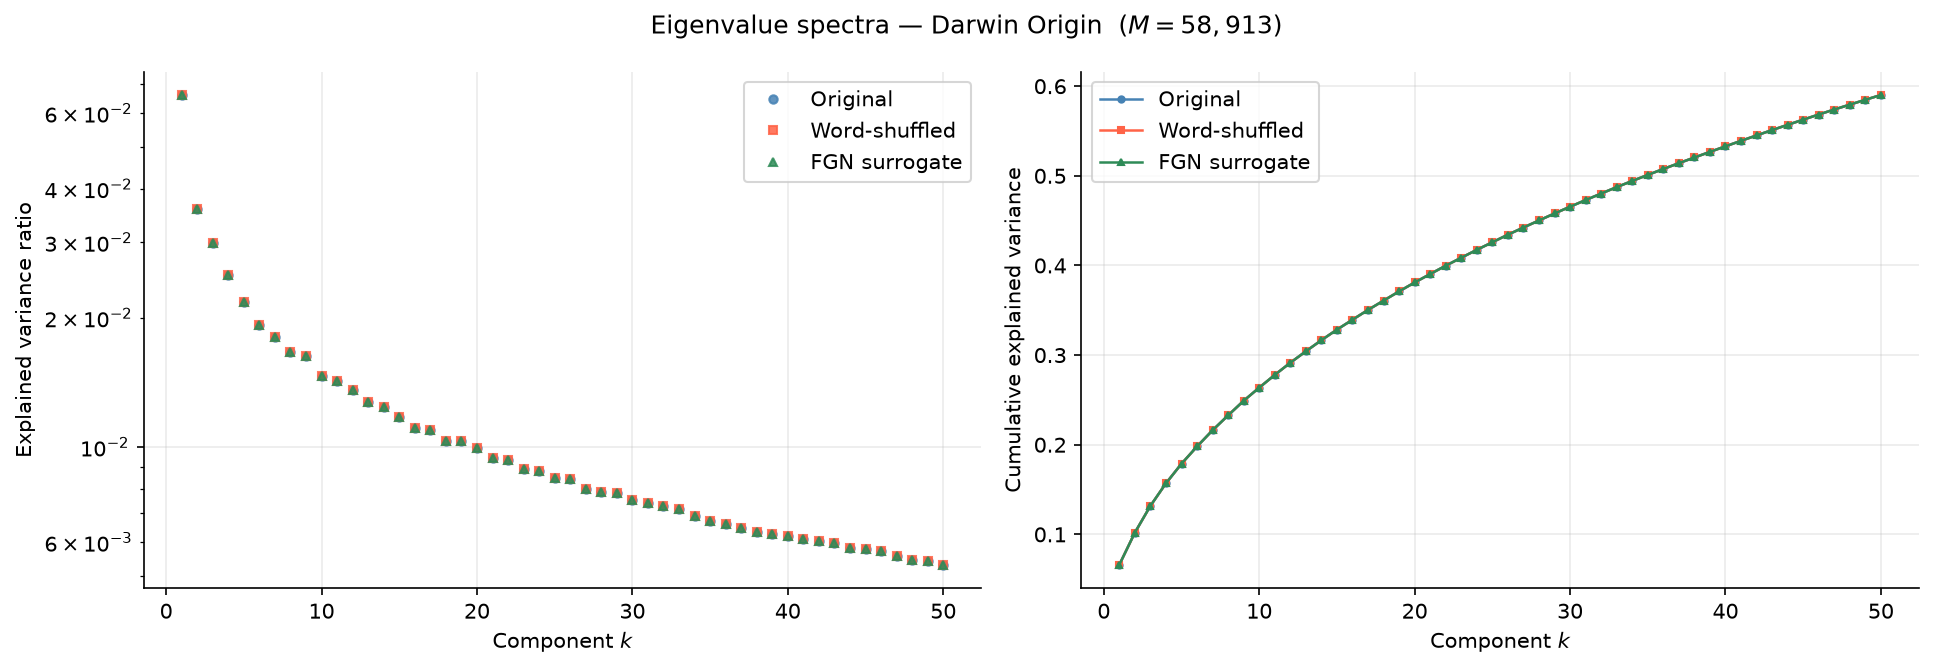
\includegraphics[width=\textwidth]{figures/darwin_origin/darwin_origin_02_spectra_comparison.png}
  \caption{Eigenvalue spectra and cumulative explained variance
  for \emph{On the Origin of Species}.
  Same conventions as Figure~\ref{fig:wrnpc_spectra}.}
  \label{fig:darwin_spectra}
\end{figure}

\begin{figure}[htbp]
  \centering
  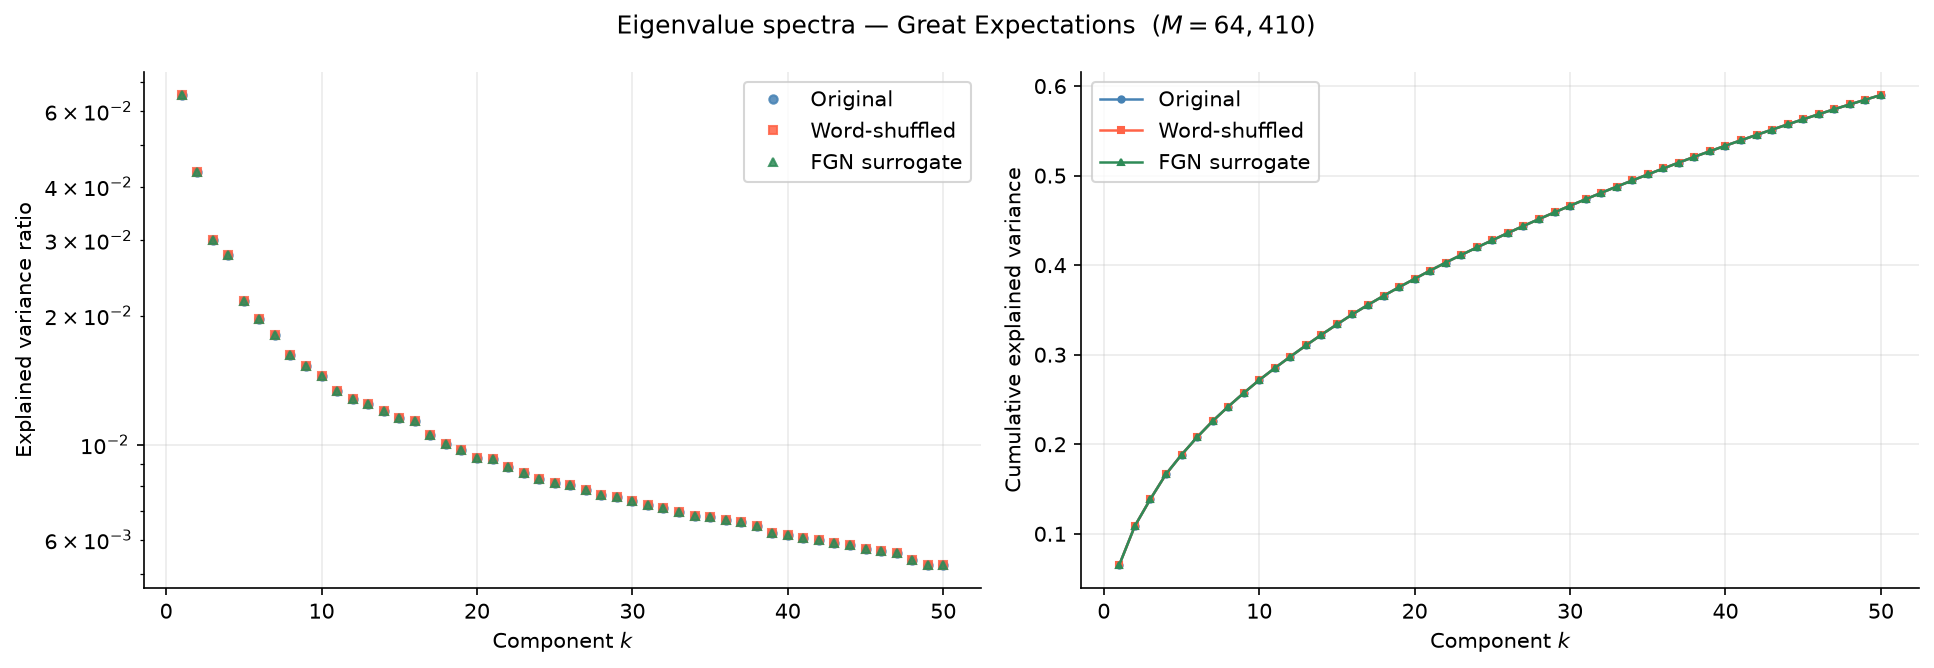
\includegraphics[width=\textwidth]{figures/great_expectations_cut_clean/great_expectations_cut_clean_02_spectra_comparison.png}
  \caption{Eigenvalue spectra and cumulative explained variance
  for \emph{Great Expectations}.
  Same conventions as Figure~\ref{fig:wrnpc_spectra}.}
  \label{fig:greatexp_spectra}
\end{figure}

\begin{figure}[htbp]
  \centering
  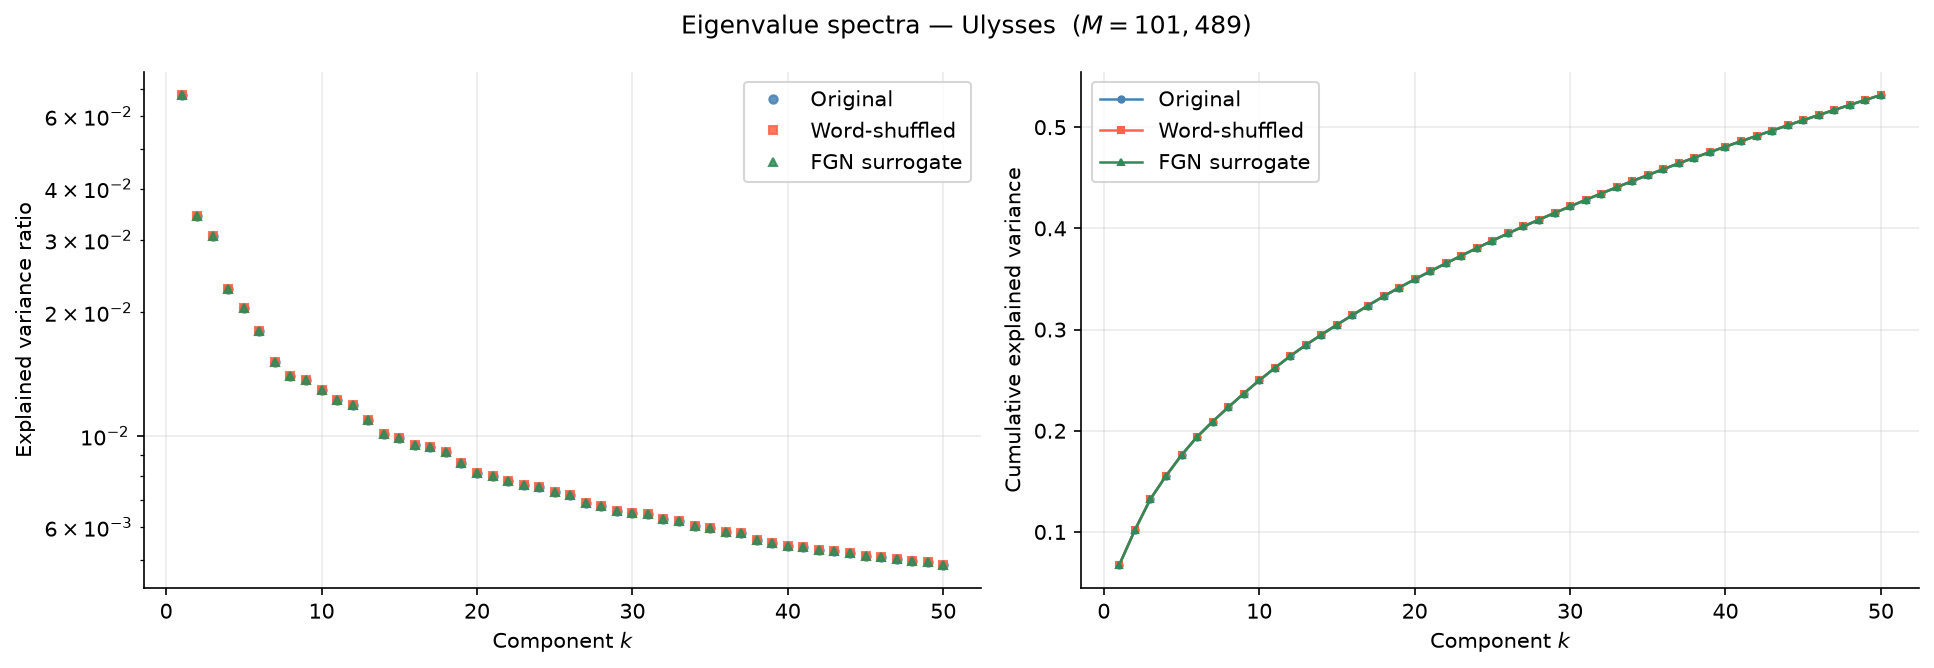
\includegraphics[width=\textwidth]{figures/eng_ulysses/eng_ulysses_02_spectra_comparison.png}
  \caption{Eigenvalue spectra and cumulative explained variance
  for \emph{Ulysses}.
  The more gradual eigenvalue decay reflects the greater stylistic
  diversity of the 18 episodes compared to the other texts.}
  \label{fig:ulysses_spectra}
\end{figure}

\begin{figure}[htbp]
  \centering
  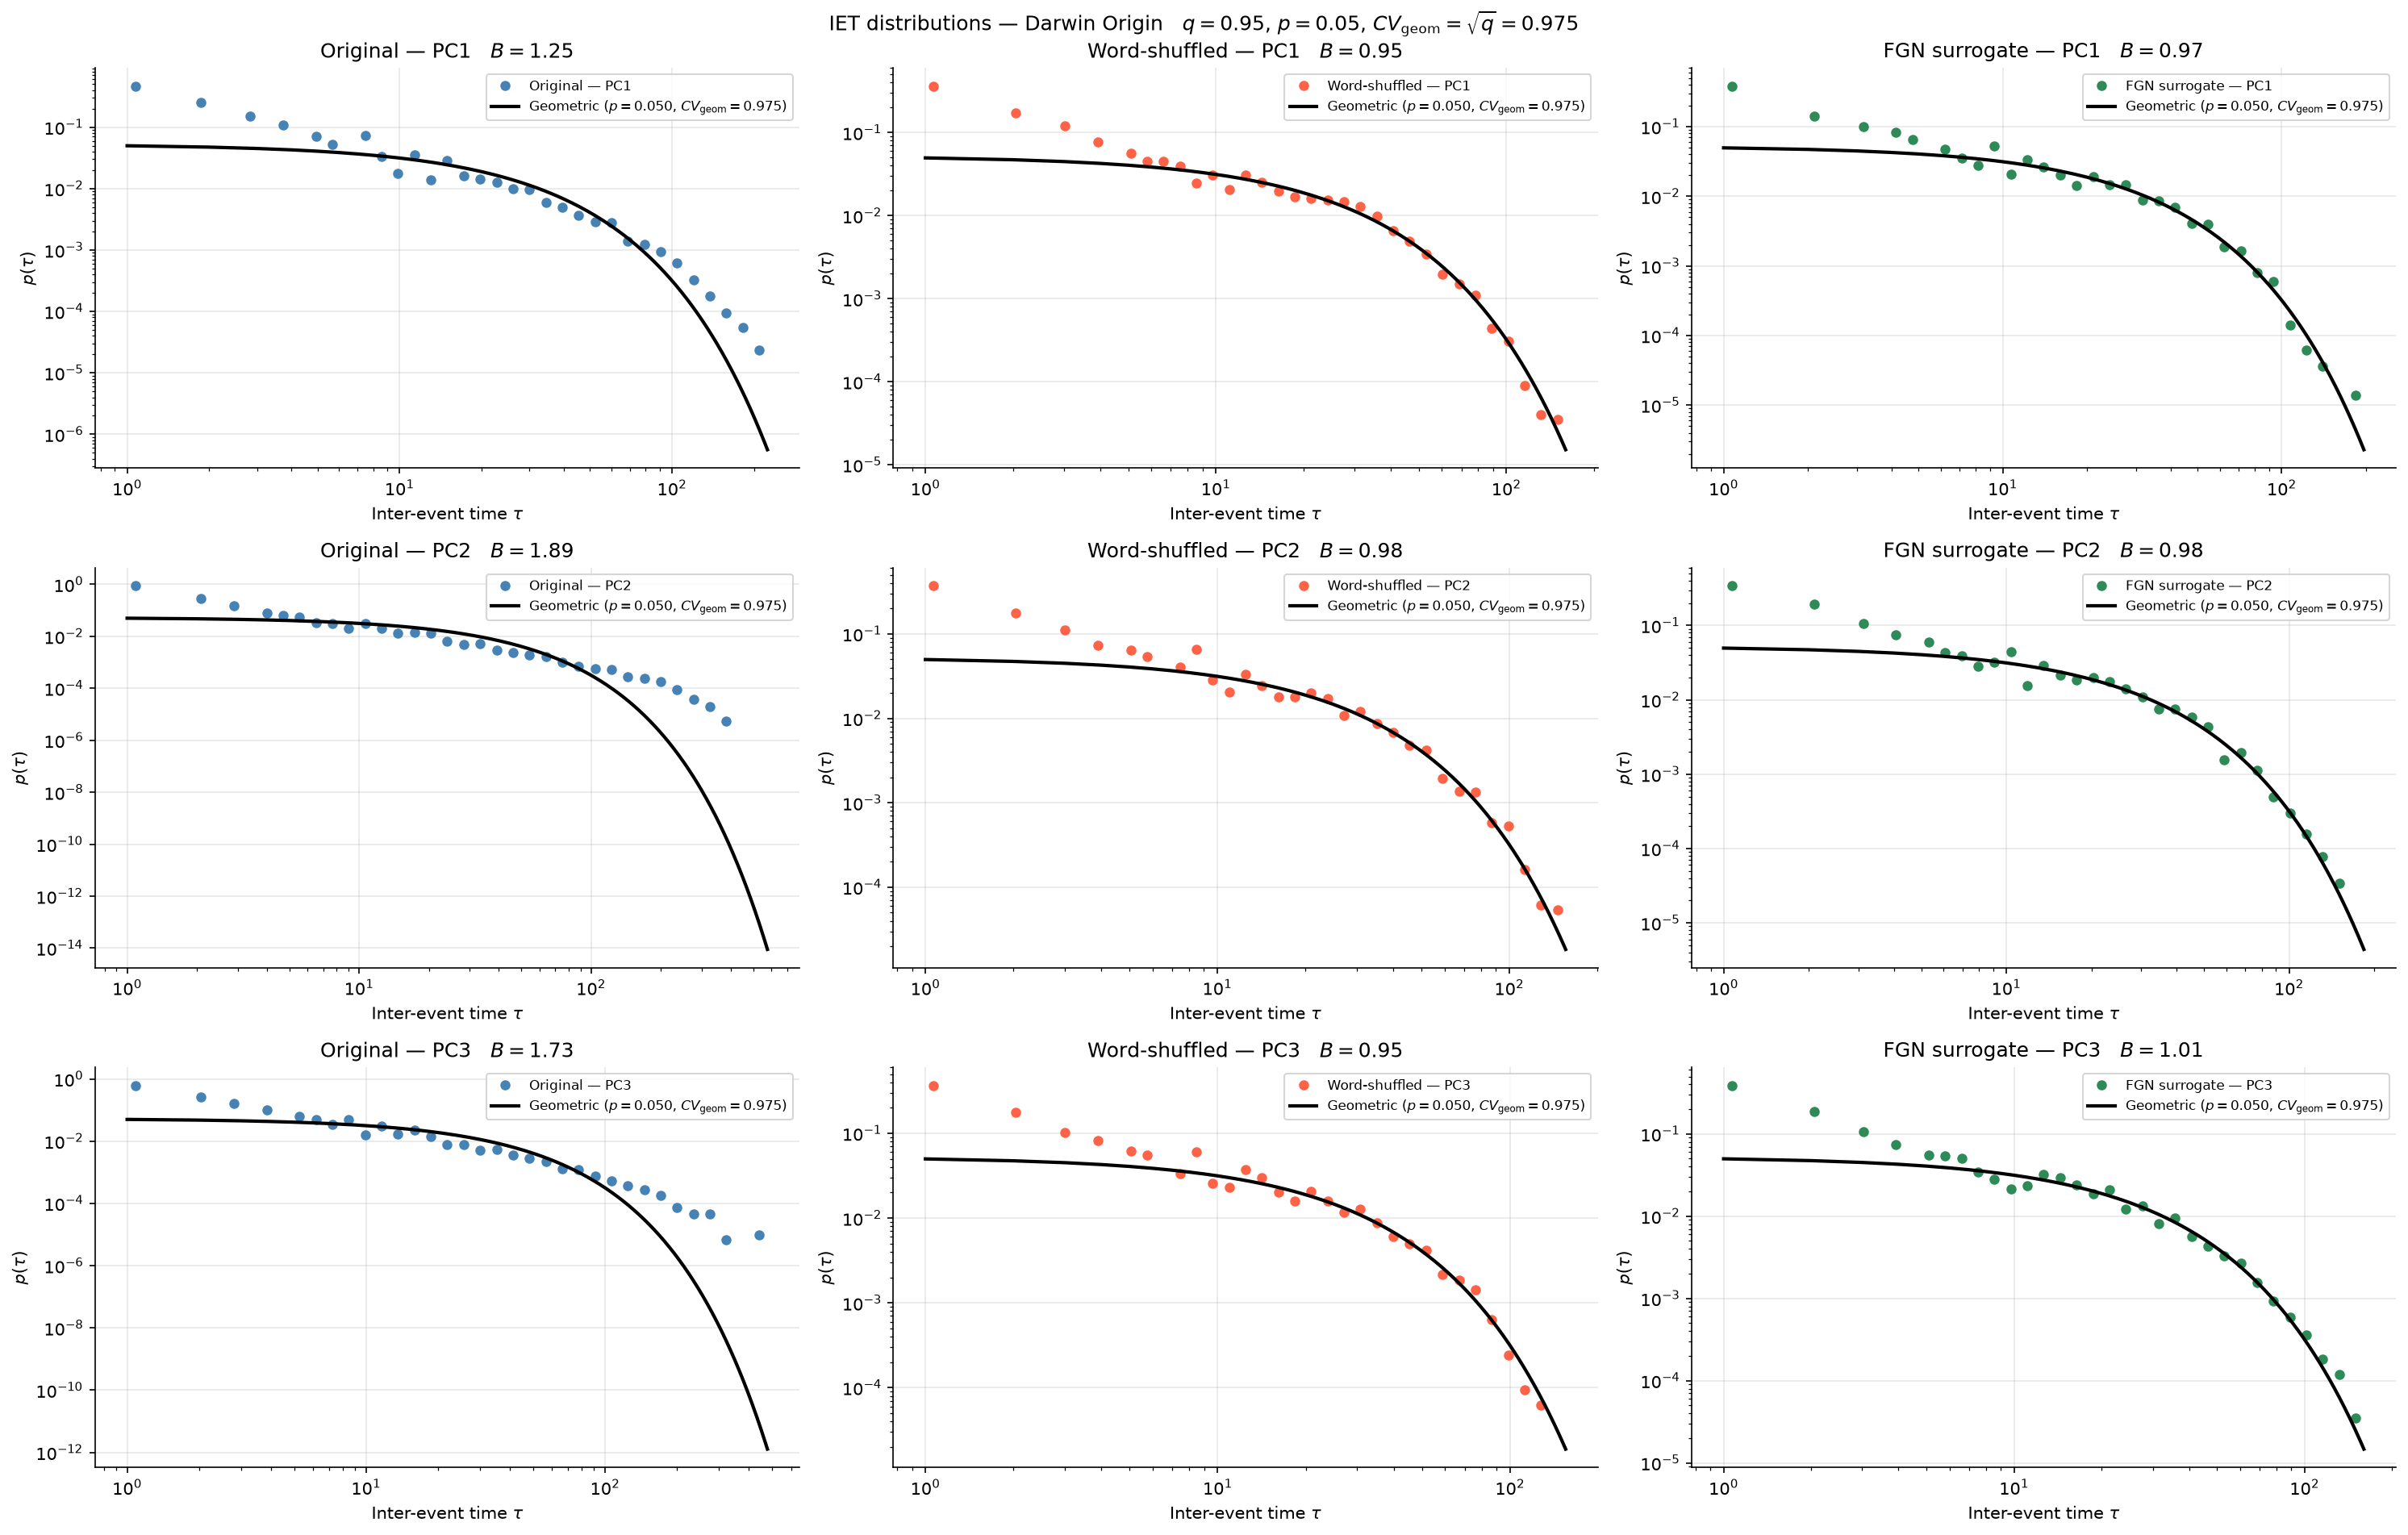
\includegraphics[width=\textwidth]{figures/darwin_origin/darwin_origin_03_iet_comparison.png}
  \caption{Inter-event time distributions for PC1, PC2, PC3 of
  \emph{On the Origin of Species} ($q=0.95$).
  Same conventions as Figure~\ref{fig:wrnpc_iet}.}
  \label{fig:darwin_iet}
\end{figure}

\begin{figure}[htbp]
  \centering
  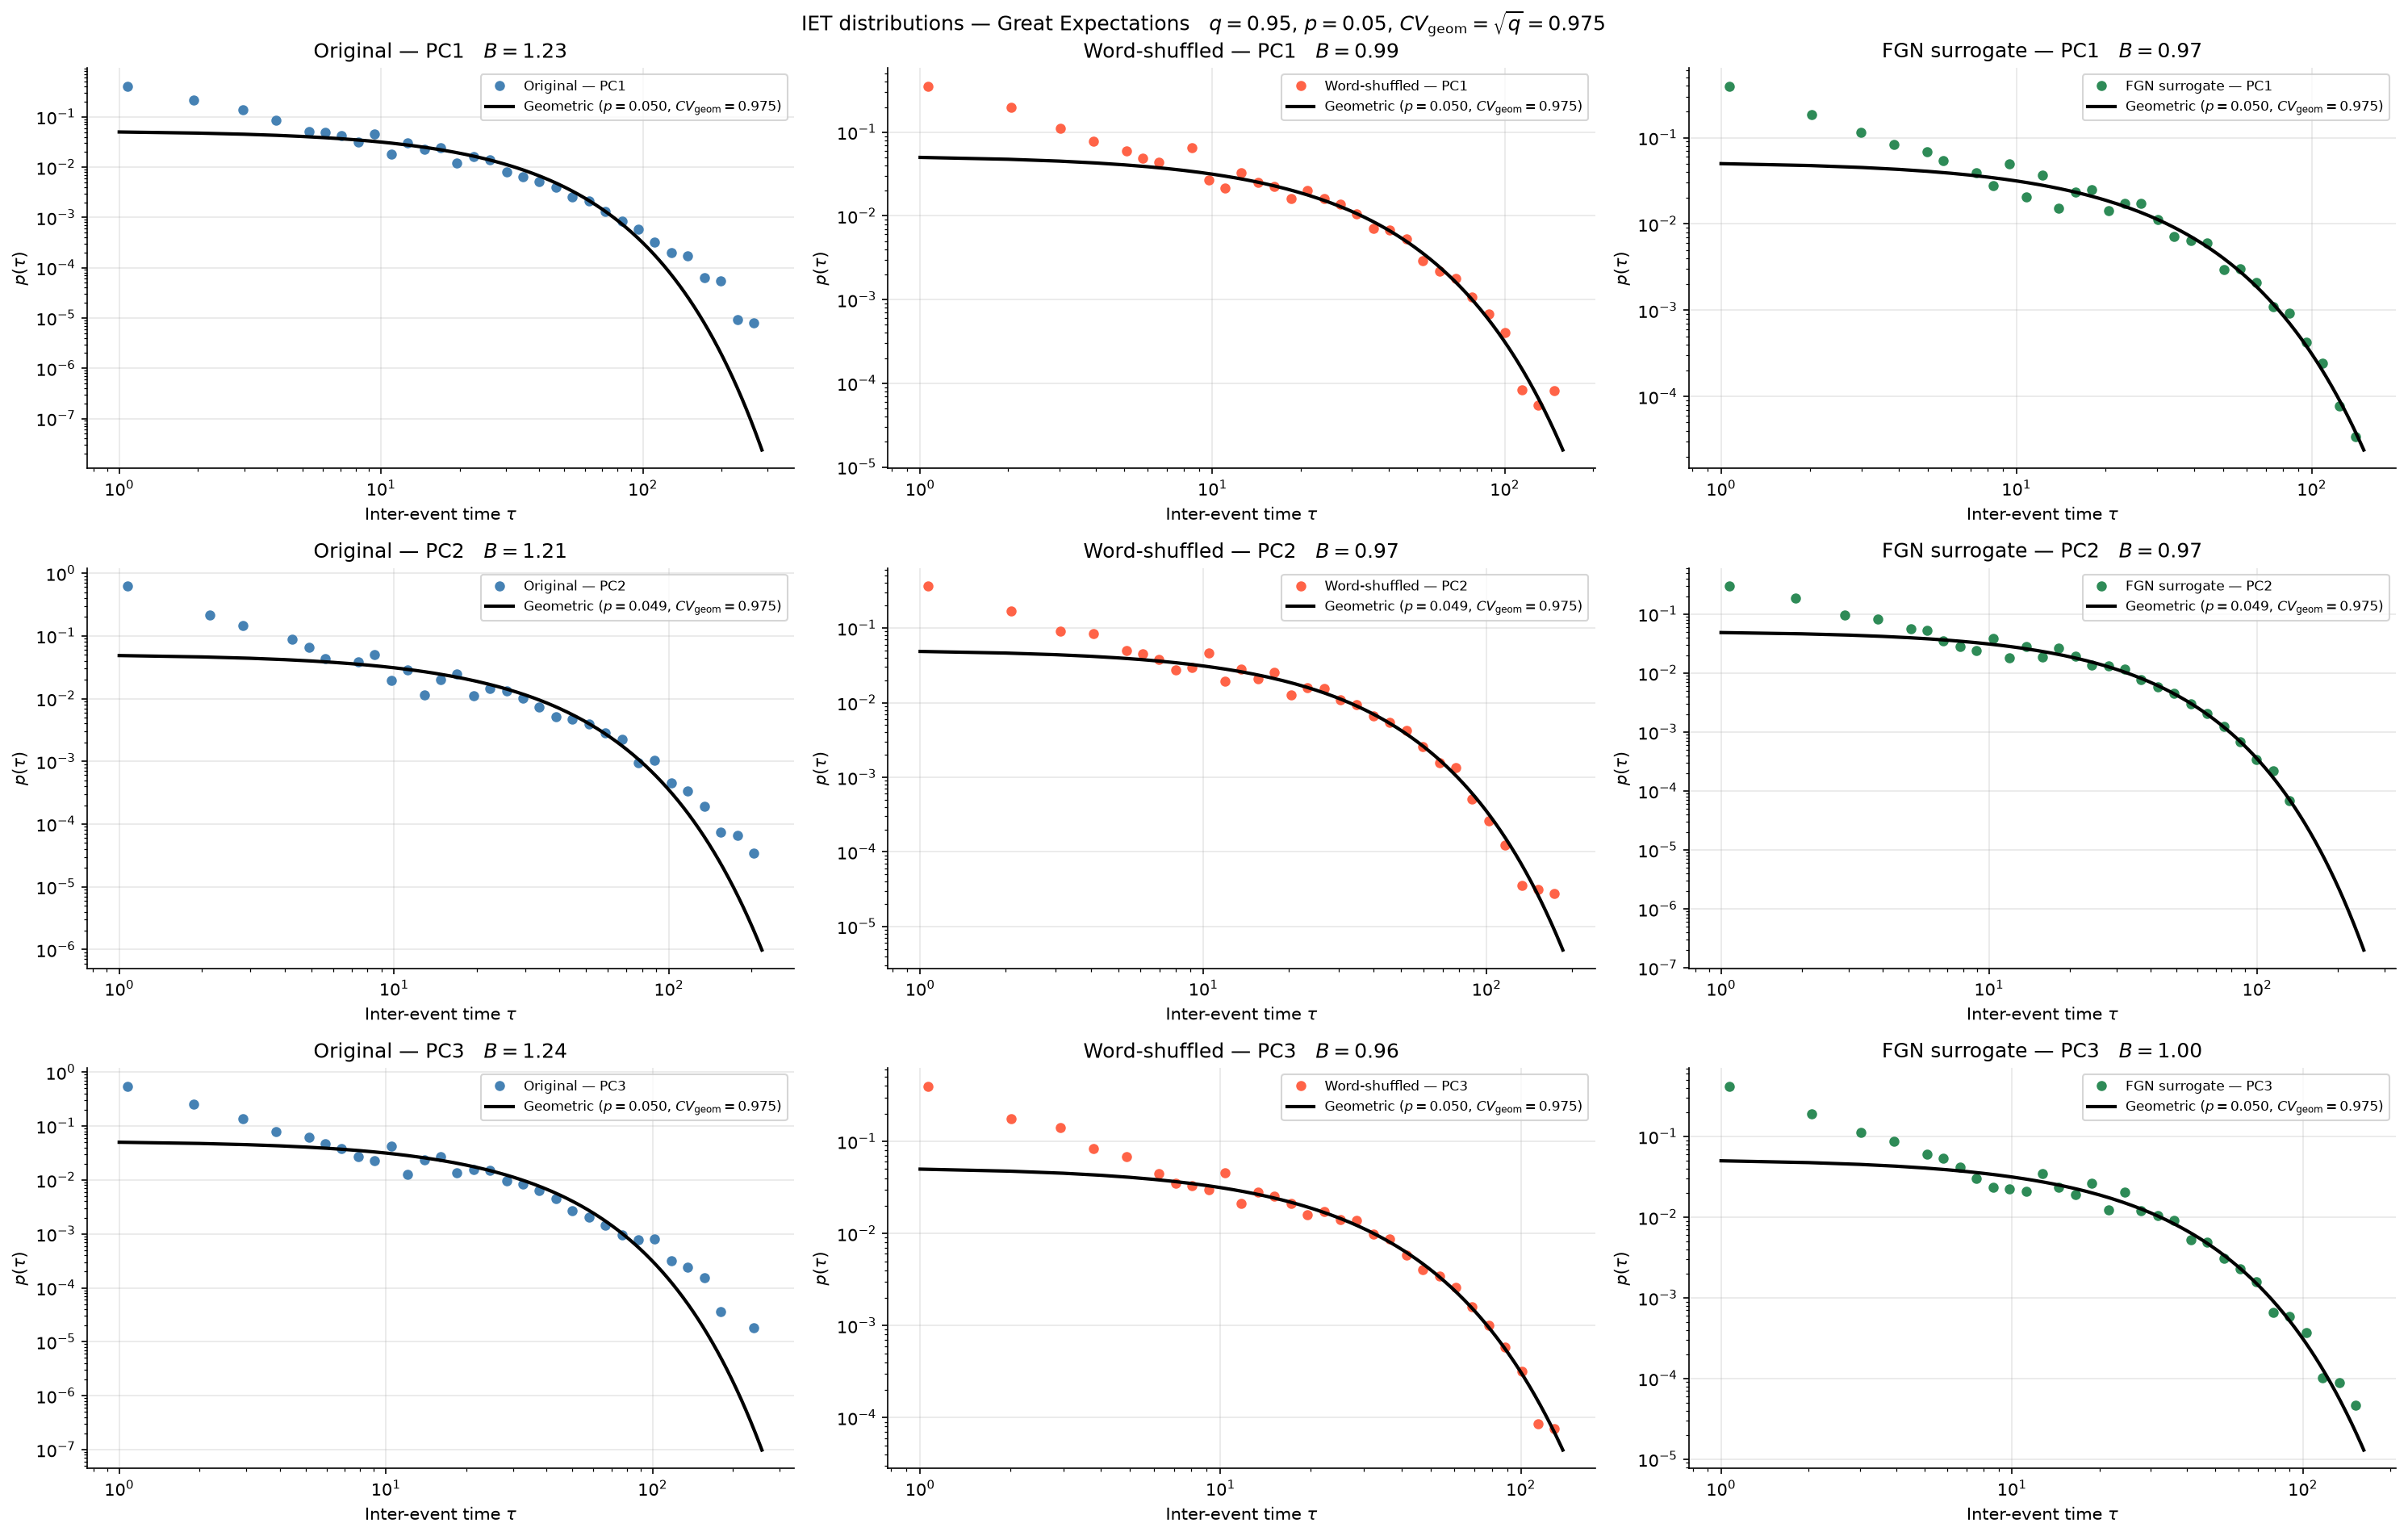
\includegraphics[width=\textwidth]{figures/great_expectations_cut_clean/great_expectations_cut_clean_03_iet_comparison.png}
  \caption{Inter-event time distributions for PC1, PC2, PC3
  of \emph{Great Expectations} ($q=0.95$).
  Same conventions as Figure~\ref{fig:wrnpc_iet}.}
  \label{fig:greatexp_iet}
\end{figure}

\begin{figure}[htbp]
  \centering
  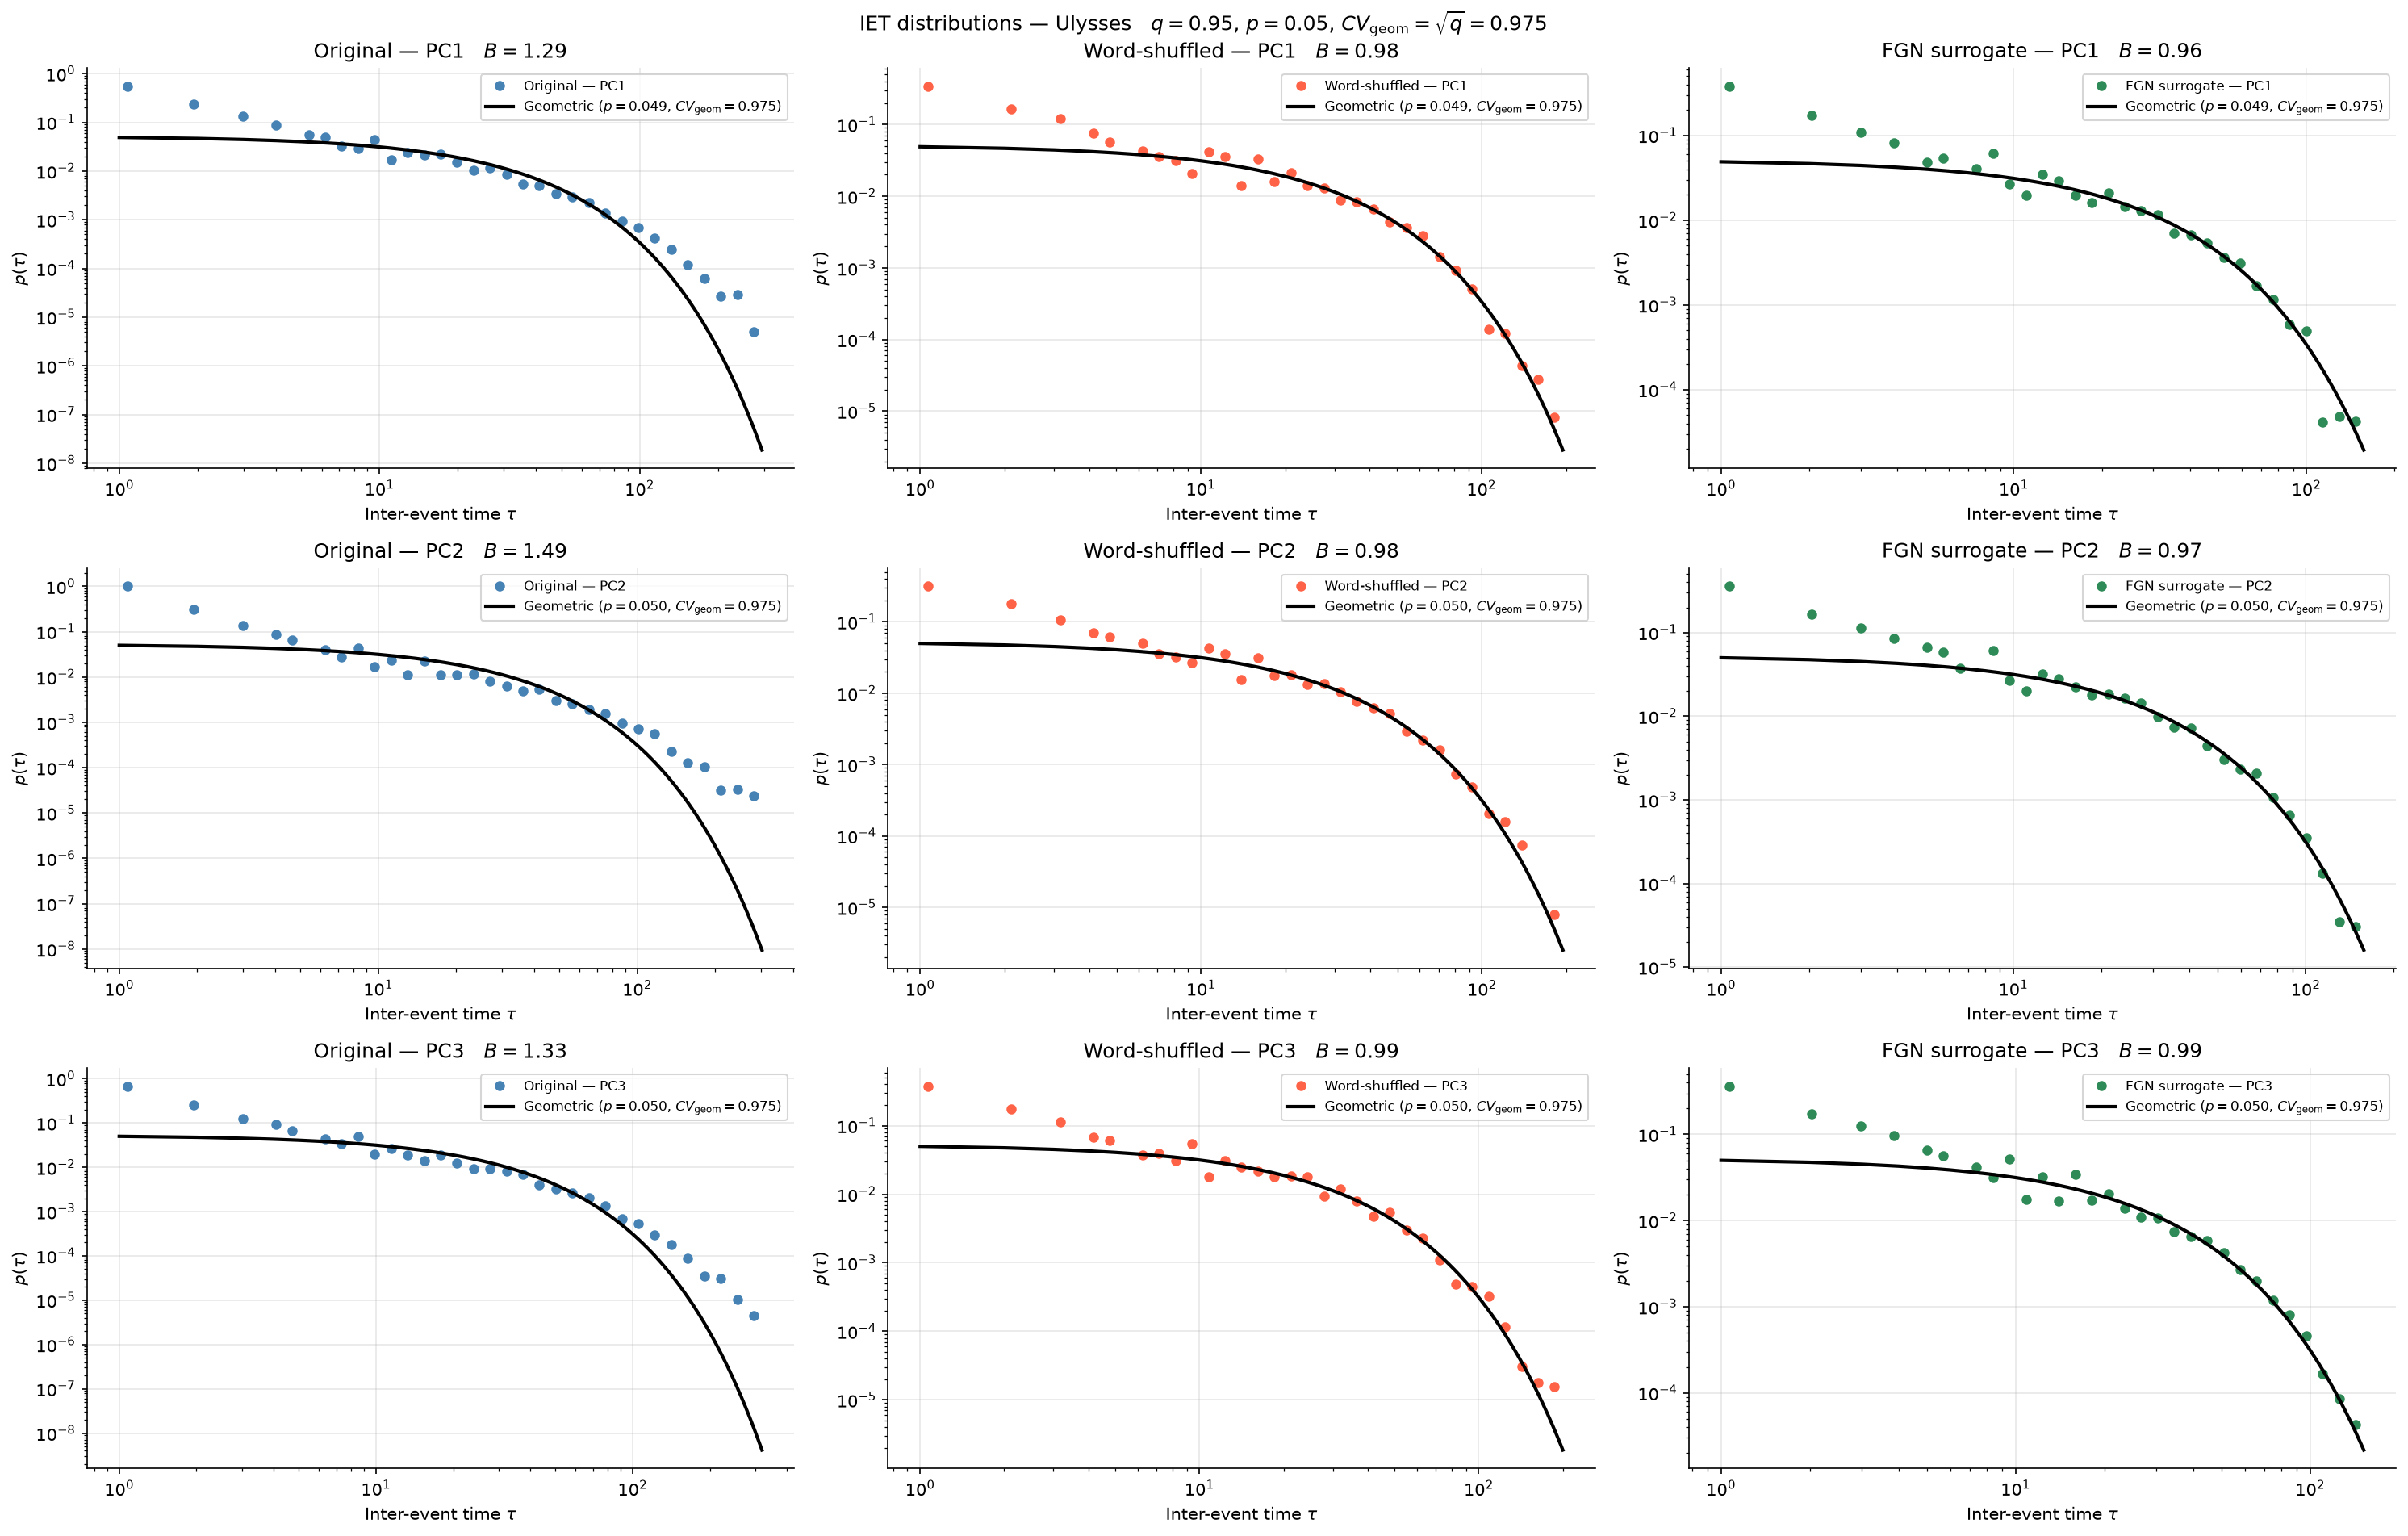
\includegraphics[width=\textwidth]{figures/eng_ulysses/eng_ulysses_03_iet_comparison.png}
  \caption{Inter-event time distributions for PC1, PC2, PC3
  of \emph{Ulysses} ($q=0.95$).
  Same conventions as Figure~\ref{fig:wrnpc_iet}.}
  \label{fig:ulysses_iet}
\end{figure}


%\section{Corpus text list}
%\label{app:corpus}
%
%\NOTE{Table already in Section~\ref{sec:corpus_texts}
%(Table~\ref{tab:corpus}).
%Appendix version to include additional columns:
%OOV rate, $\alpha_0$ (FGN bisection parameter).
%\TODO{Copy and extend from main table.}}


% ──────────────────────────────────────────────────────────
\bibliographystyle{apalike}
\begin{thebibliography}{99}

\bibitem[Alvarez-Lacalle et~al.(2006)]{AlvarezLacalle2006}
Alvarez-Lacalle, E., Dorow, B., Eckmann, J.-P., and Moses, E. (2006).
\newblock Hierarchical structures induce long-range dynamical correlations in written texts.
\newblock \emph{Proceedings of the National Academy of Sciences},
  103(21):7956--7961.

\bibitem[Altmann et~al.(2012)]{Altmann2012}
Altmann, E.~G., Cristadoro, G., and Degli~Esposti, M. (2012).
\newblock On the origin of long-range correlations in texts.
\newblock \emph{Proceedings of the National Academy of Sciences},
  109(29):11582--11587.

\bibitem[Degli~Esposti and Montemurro(2025)]{DegliEsposti2025}
Degli~Esposti, M. and Montemurro, M.~A. (2025).
\newblock A {Z}ipf-preserving, long-range correlated surrogate for
  written language and other symbolic sequences.
\newblock \emph{Physica A: Statistical Mechanics and its Applications}.

\bibitem[Ebeling and Neiman(1995)]{Ebeling1995}
Ebeling, W. and Neiman, A. (1995).
\newblock Long-range correlations between letters and sentences in
  texts.
\newblock \emph{Physica A}, 215:233--241.

\bibitem[Goh and Barab{\'a}si(2008)]{GohBarabasi2008}
Goh, K.-I. and Barab{\'a}si, A.-L. (2008).
\newblock Burstiness and memory in complex systems.
\newblock \emph{Europhysics Letters}, 81:48002.

\bibitem[Mikolov et~al.(2013)]{Mikolov2013}
Mikolov, T., Sutskever, I., Chen, K., Corrado, G.~S., and Dean, J.
  (2013).
\newblock Distributed representations of words and phrases and their
  compositionality.
\newblock In \emph{Advances in Neural Information Processing Systems},
  volume~26.

\bibitem[Montemurro and Degli~Esposti(2025)]{MontemurroDegliEsposti2025}
Montemurro, M.~A. and Degli~Esposti, M. (2025).
\newblock Long-range correlations in {H}eap's law fluctuations.
\newblock \emph{In preparation}.

\bibitem[Montemurro and Pury(2002)]{MontemurroPury2002}
Montemurro, M.~A. and Pury, P.~A. (2002).
\newblock Long-range fractal correlations in literary corpora.
\newblock \emph{Fractals}, 10:451--461.

\bibitem[Peng et~al.(1994)]{Peng1994}
Peng, C.-K., Buldyrev, S.~V., Havlin, S., Simons, M., Stanley,
  H.~E., and Goldberger, A.~L. (1994).
\newblock Mosaic organization of {DNA} nucleotides.
\newblock \emph{Physical Review E}, 49(2):1685--1689.

\bibitem[Pennington et~al.(2014)]{Pennington2014}
Pennington, J., Socher, R., and Manning, C.~D. (2014).
\newblock {G}lo{V}e: Global vectors for word representation.
\newblock In \emph{Proceedings of EMNLP}, pages 1532--1543.

\bibitem[Zipf(1949)]{Zipf1949}
Zipf, G.~K. (1949).
\newblock \emph{Human Behavior and the Principle of Least Effort}.
\newblock Addison-Wesley.

\end{thebibliography}

\end{document}
